\section{作用力測定装置の評価実験とその考察}

製作した校正実験装置を用いて行った作用力測定装置の性能評価実験について説明する.

\subsection{実験方法}

作用力測定装置の性能を調べるために,複数の角度からのデータを使用し結果を得る必要があり,
結果の再現性,一般性を確保するためには評価実験を複数回繰り返さなければならない.
大量のデータをプログラムで一度に処理できるようにするため,測定手順を以下のように定めた.

\subsubsection{試行回数と測定角度}
本研究で行った実験についての測定角度および試行回数を以下のTable に示す.

\begin{table}[htbp]
	\begin{center}
		\caption{Experiment conditions}
		\begin{tabular}{|p{30mm}|p{20mm}|p{30}|}
			\hline
			\multicolumn{1}{|c|}{}                  & \multicolumn{1}{|c|}{\textgt{Condition number}} & \multicolumn{1}{|c|}{\textgt{remarks}}          \\ \hline
			\multicolumn{1}{|c|}{Measurement angle} & \multicolumn{1}{|c|}{24}                        & \multicolumn{1}{|c|}{Mesurement every 15 [deg]} \\ \hline
			\multicolumn{1}{|c|}{Number of trials}  & \multicolumn{1}{|c|}{7}                         & \multicolumn{1}{|c|}{}                          \\ \hline
		\end{tabular}
	\end{center}
\end{table}
\subsubsection{測定条件}
\begin{enumerate}[(1)]
	\item サンプリング周期は5[Hz]とする
	\item ロードセルをマイクロステージを用いて 0.03 [mm] ずつ移動させ,ひずみセンサ,\\
	      ロードセルの出力電圧を測定する
	\item 基準を0 [mm]として,0.03 [mm],0.06 [mm],0.09 [mm],0.12 [mm]の計4回移動させる
\end{enumerate}
\subsubsection{測定準備}
\begin{enumerate}[(1)]
	\item 自動回転ステージを用いてロードセルを測定する角度に固定する
	\item 自動一軸ステージを用いてロードセルが供試体に接触する位置を0.01[mm]単位で特定する
	\item 接触する前の位置を基準に測定を開始する
\end{enumerate}
\subsubsection{測定手順}
\begin{enumerate}[(1)]
	\item 測定開始から60秒間待機する
	\item 40秒間の出力電圧の測定
	\item 60秒間の自動ステージ動作時間 (※ 自動ステージ動作後,電圧の安定を図るため)
	\item (2),(3)の作業を5回繰り返す (5回目はロードセル,供試体を非接触状態にする)
\end{enumerate}

\subsection{実験結果}

上述の手順にしたがって,各角度ごとに行った測定結果を以下のFig.~Fig.に示す.
なお,以下に示す結果は1回目の測定結果における 0,30, 45,60, 90, 180 [deg]である.

  \begin{figure}[htbp]
        \begin{minipage}[b]{0.45\linewidth}
          \centering
          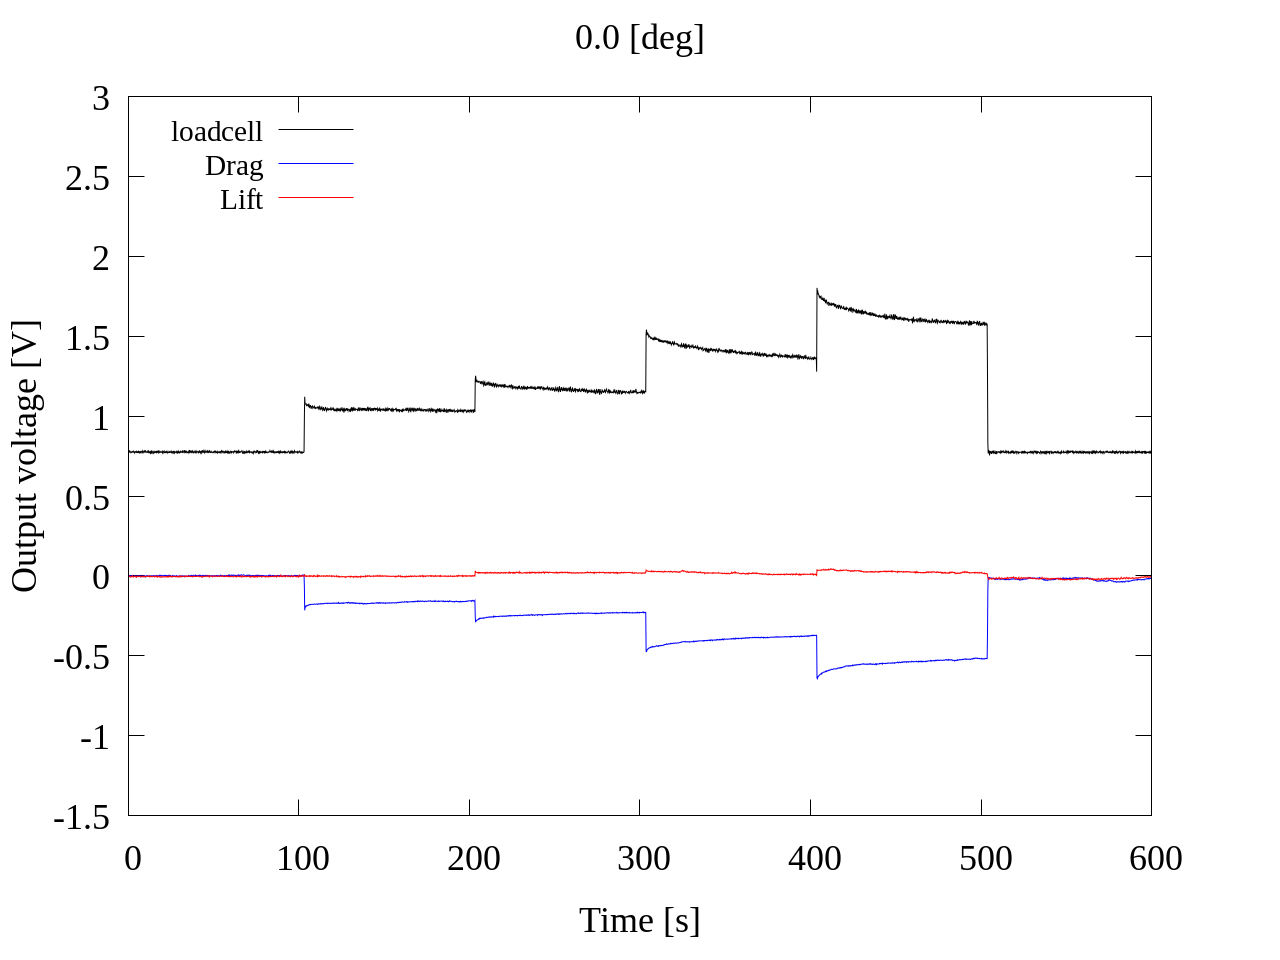
\includegraphics[width=65mm]{../../02_workspace/result/2-1/plot/01-3_allsensors/01_allsensors_0.png}
          \subcaption{0 [deg]}
        \end{minipage}
        \begin{minipage}[b]{0.45\linewidth}
          \centering
          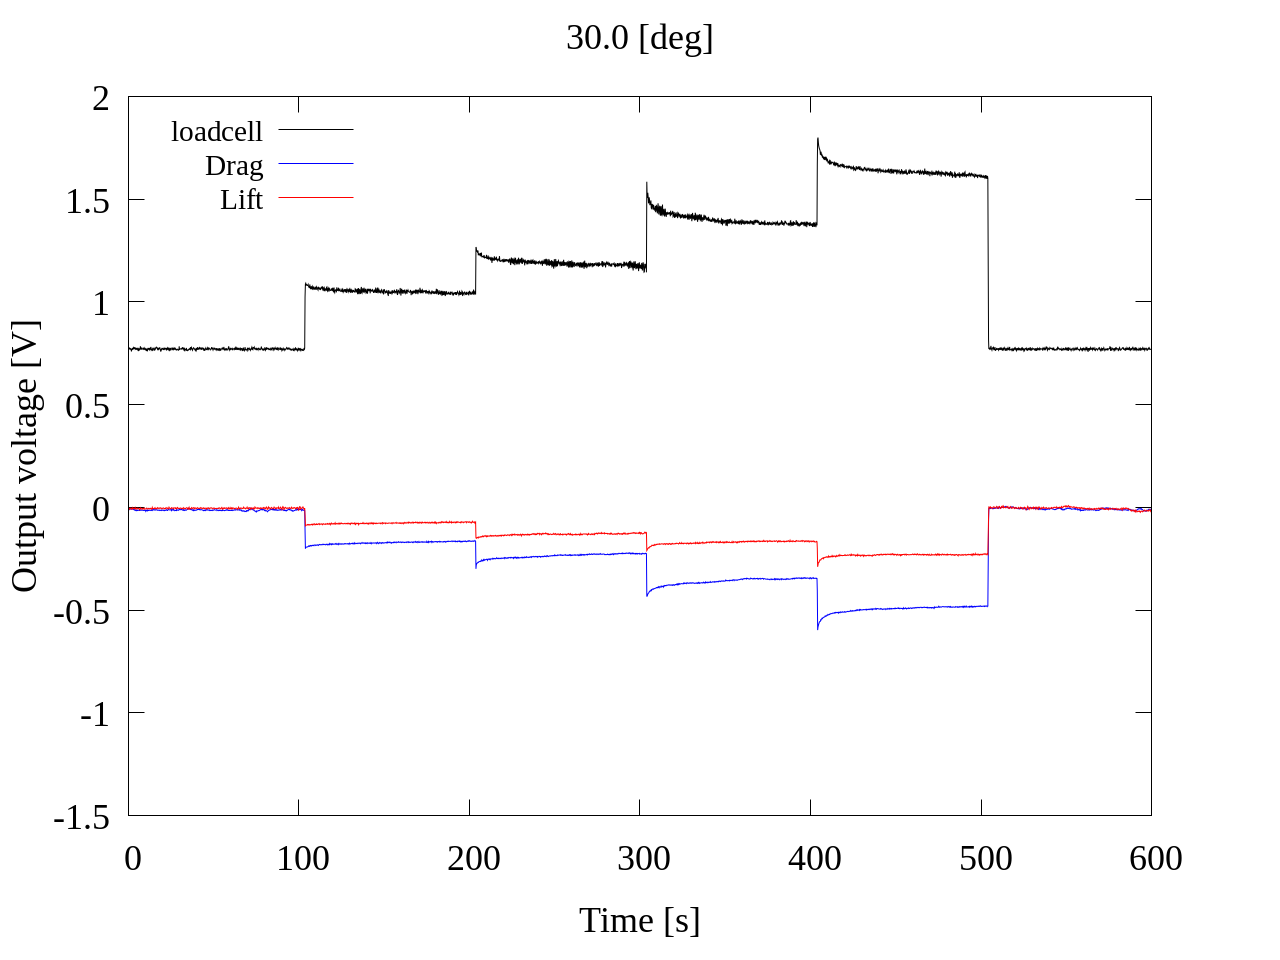
\includegraphics[width=65mm]{../../02_workspace/result/2-1/plot/01-3_allsensors/01_allsensors_300.png}
          \subcaption{30 [deg]}
        \end{minipage} \\
        \begin{minipage}[b]{0.45\linewidth}
            \centering
            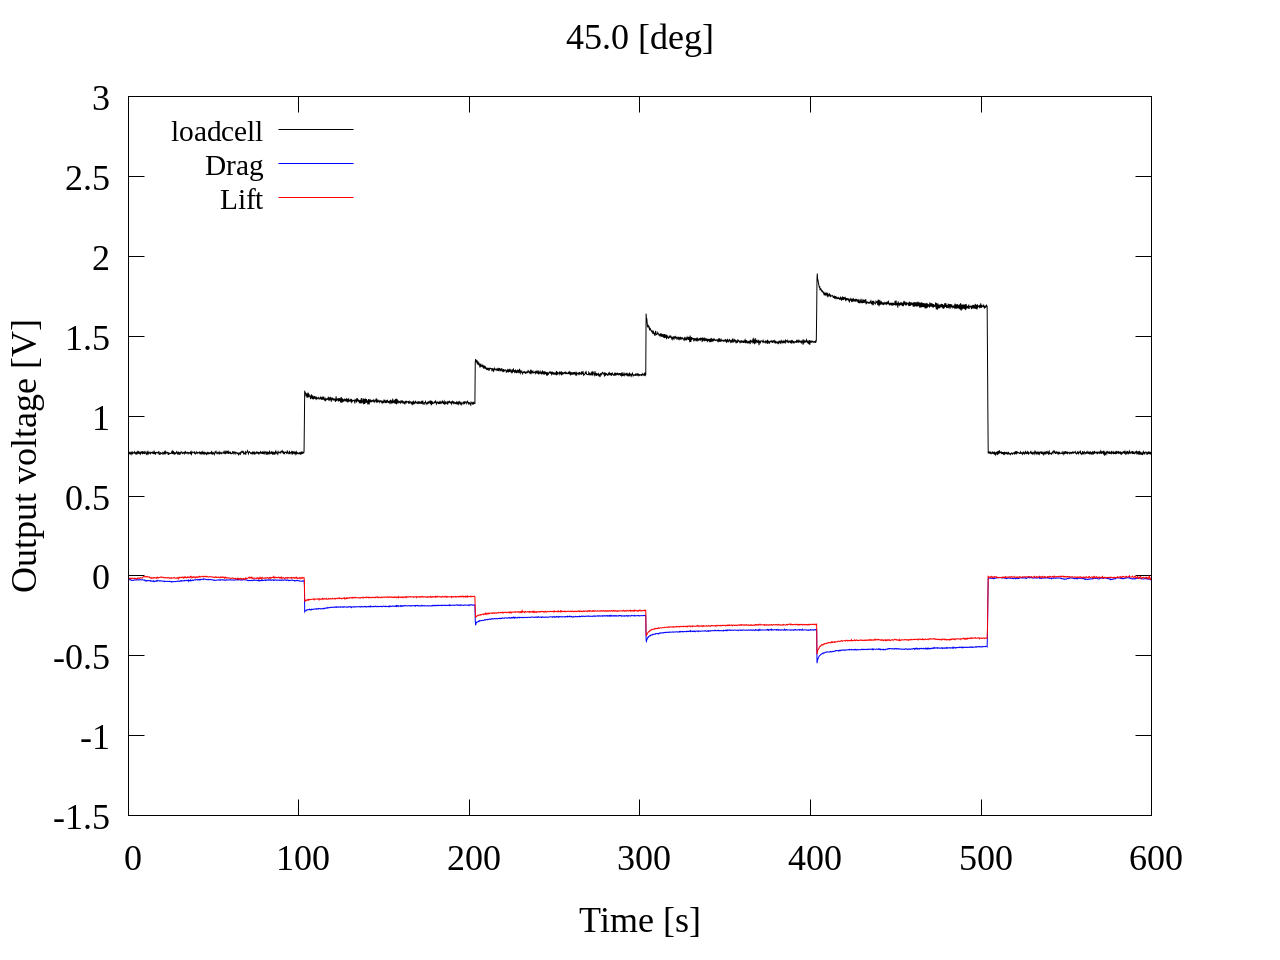
\includegraphics[width=65mm]{../../02_workspace/result/2-1/plot/01-3_allsensors/01_allsensors_450.png}
            \subcaption{45 [deg]}
          \end{minipage}
          \begin{minipage}[b]{0.45\linewidth}
            \centering
            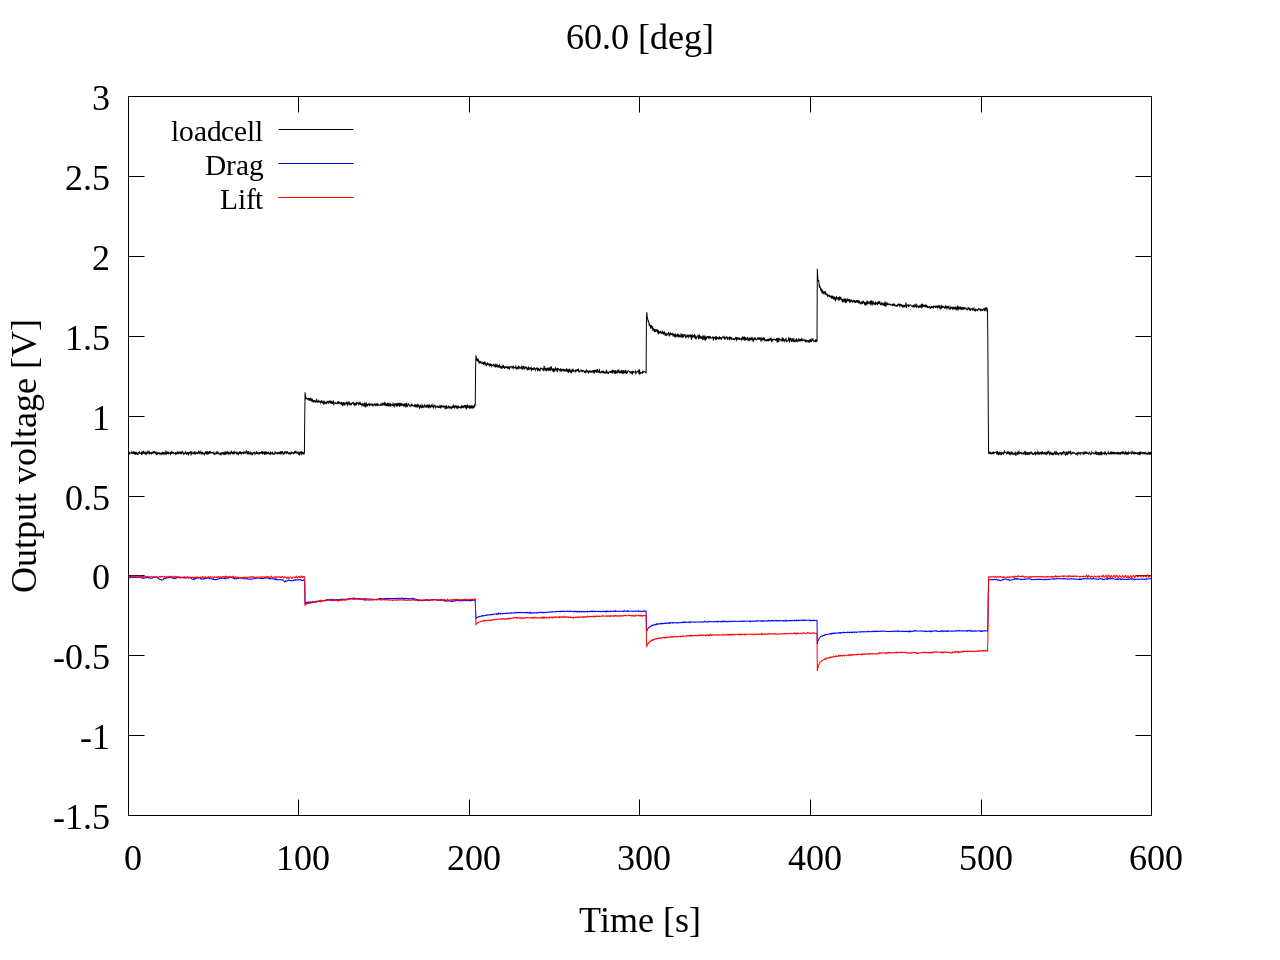
\includegraphics[width=65mm]{../../02_workspace/result/2-1/plot/01-3_allsensors/01_allsensors_600.png}
            \subcaption{60 [deg]}
          \end{minipage}\\
          \begin{minipage}[b]{0.45\linewidth}
            \centering
            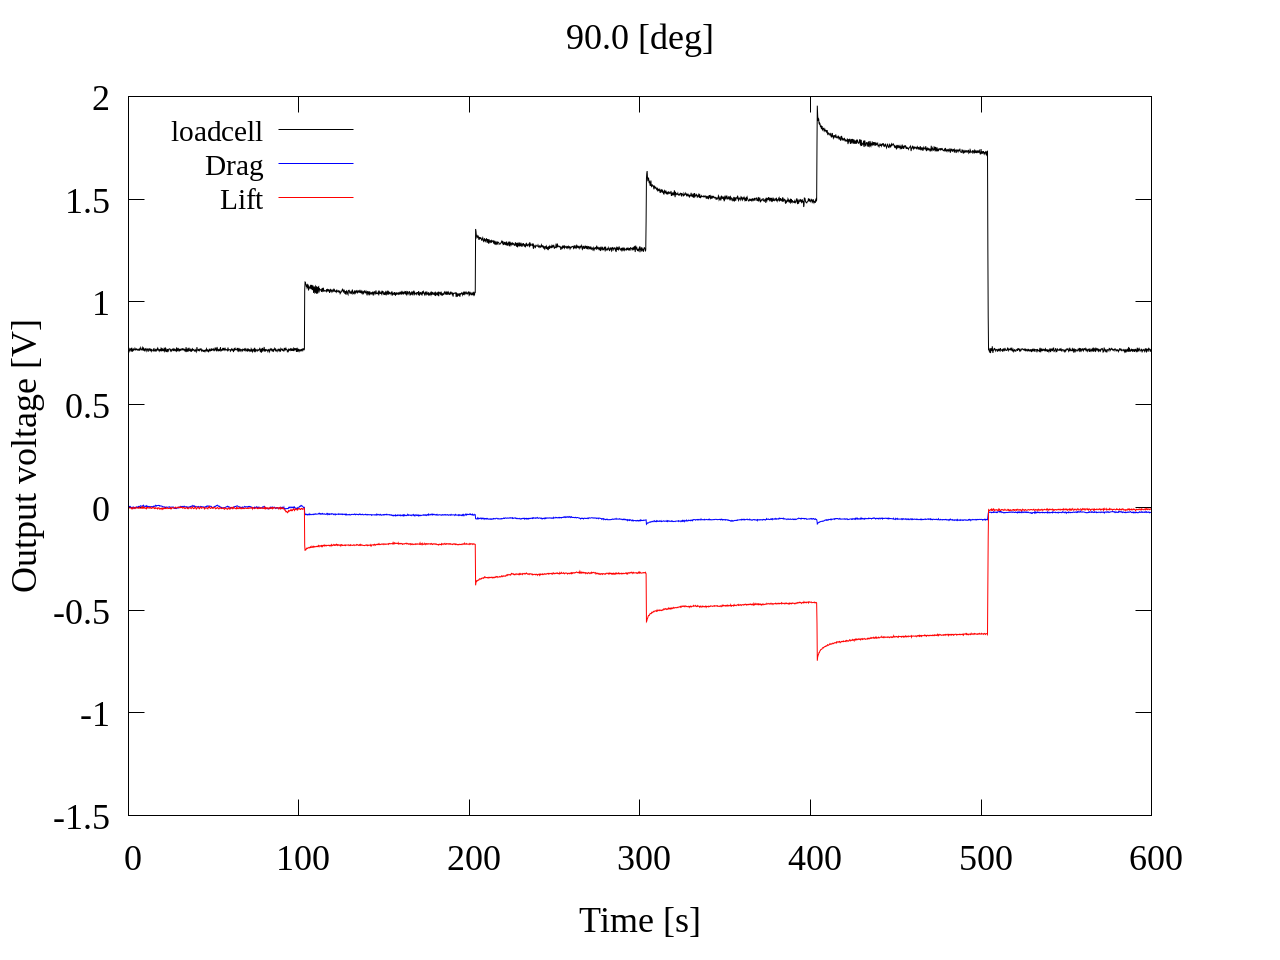
\includegraphics[width=65mm]{../../02_workspace/result/2-1/plot/01-3_allsensors/01_allsensors_900.png}
            \subcaption{90 [deg]}
          \end{minipage}
          \begin{minipage}[b]{0.45\linewidth}
            \centering
            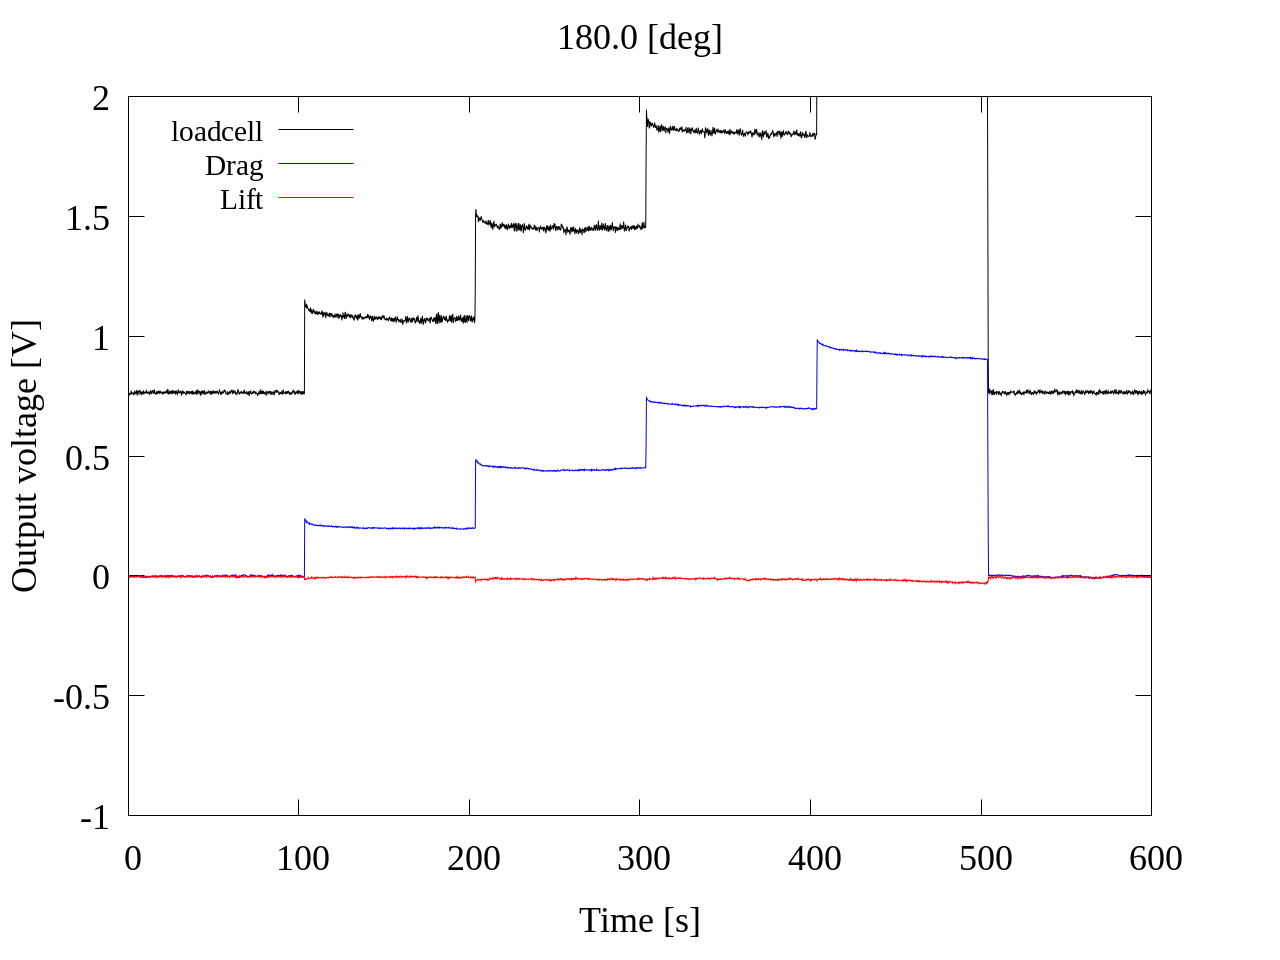
\includegraphics[width=65mm]{../../02_workspace/result/2-1/plot/01-3_allsensors/01_allsensors_1800.png}
            \subcaption{180 [deg]}
          \end{minipage} 
          \caption{Output voltage}
    \end{figure}

% \begin{figure}[htbp]
%     \begin{minipage}[b]{0.45\linewidth}
%       \centering
%       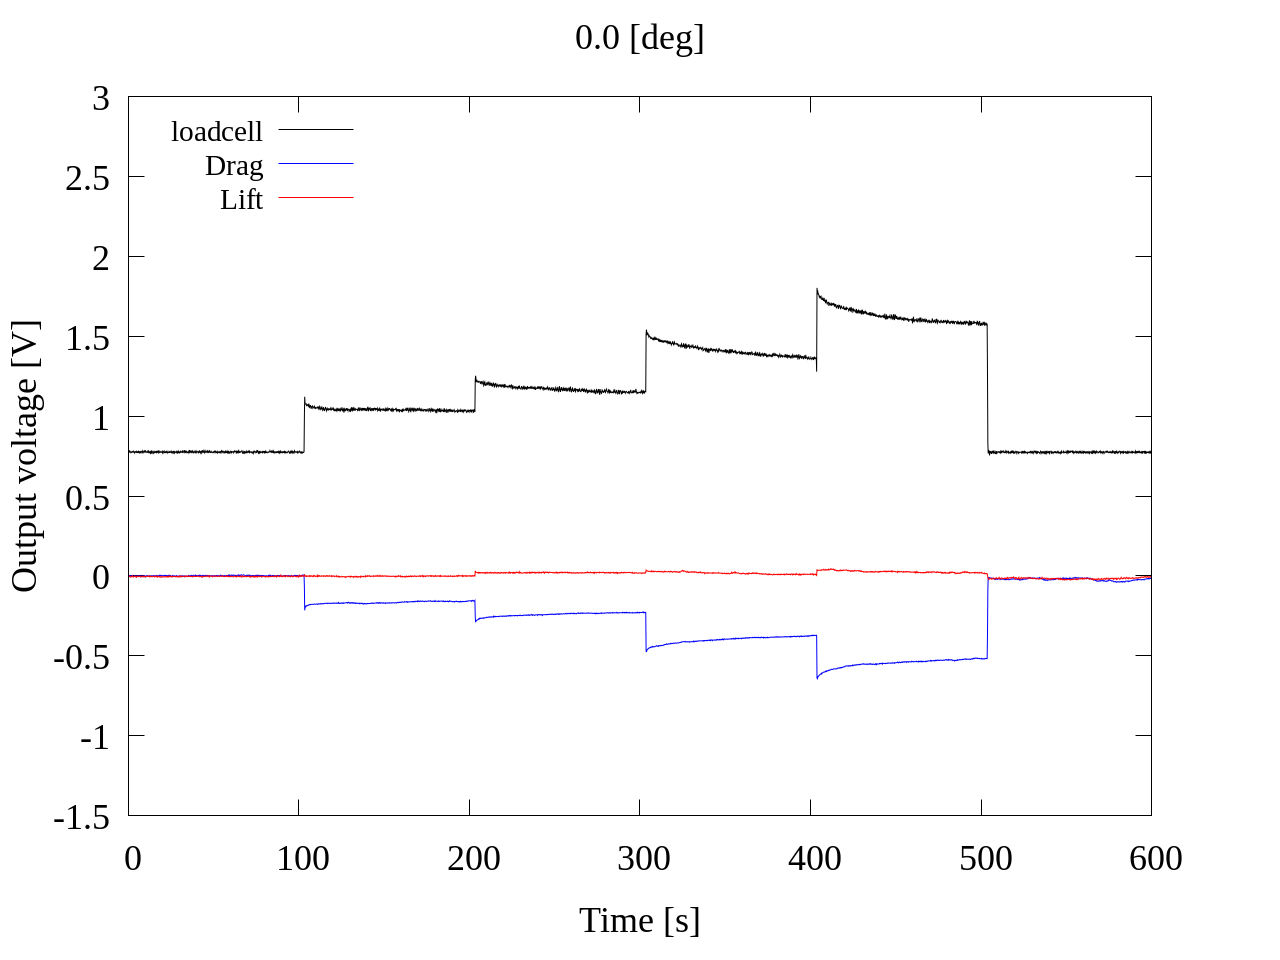
\includegraphics[width=65mm]{../../02_workspace/result/2-1/plot/01-3_allsensors/01_allsensors_0.png}
%       \subcaption{0 [deg]}
%     \end{minipage}
%     \begin{minipage}[b]{0.45\linewidth}
%       \centering
%       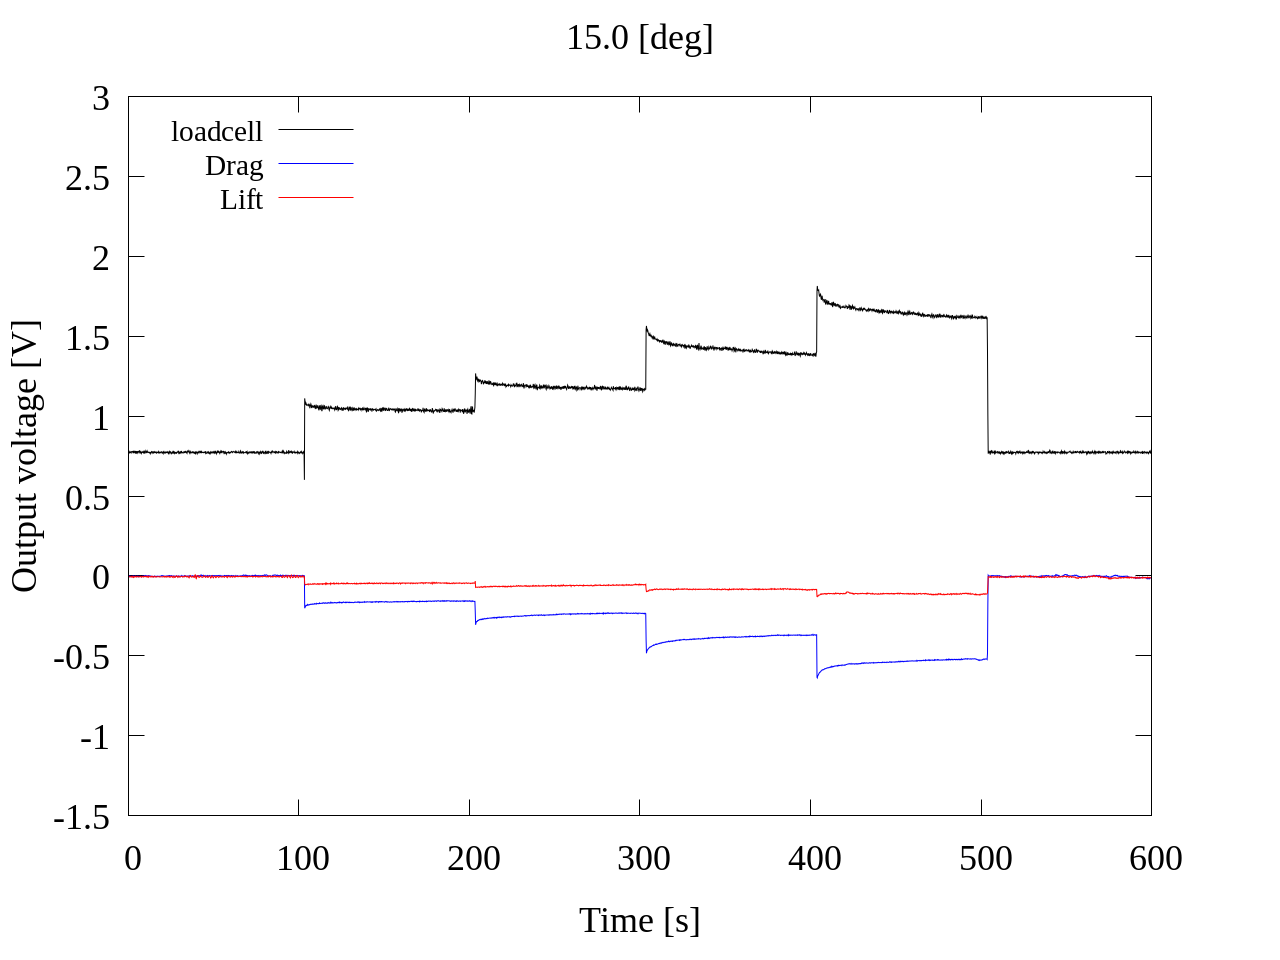
\includegraphics[width=65mm]{../../02_workspace/result/2-1/plot/01-3_allsensors/01_allsensors_150.png}
%       \subcaption{15 [deg]}
%     \end{minipage} \\
%     \begin{minipage}[b]{0.45\linewidth}
%         \centering
%         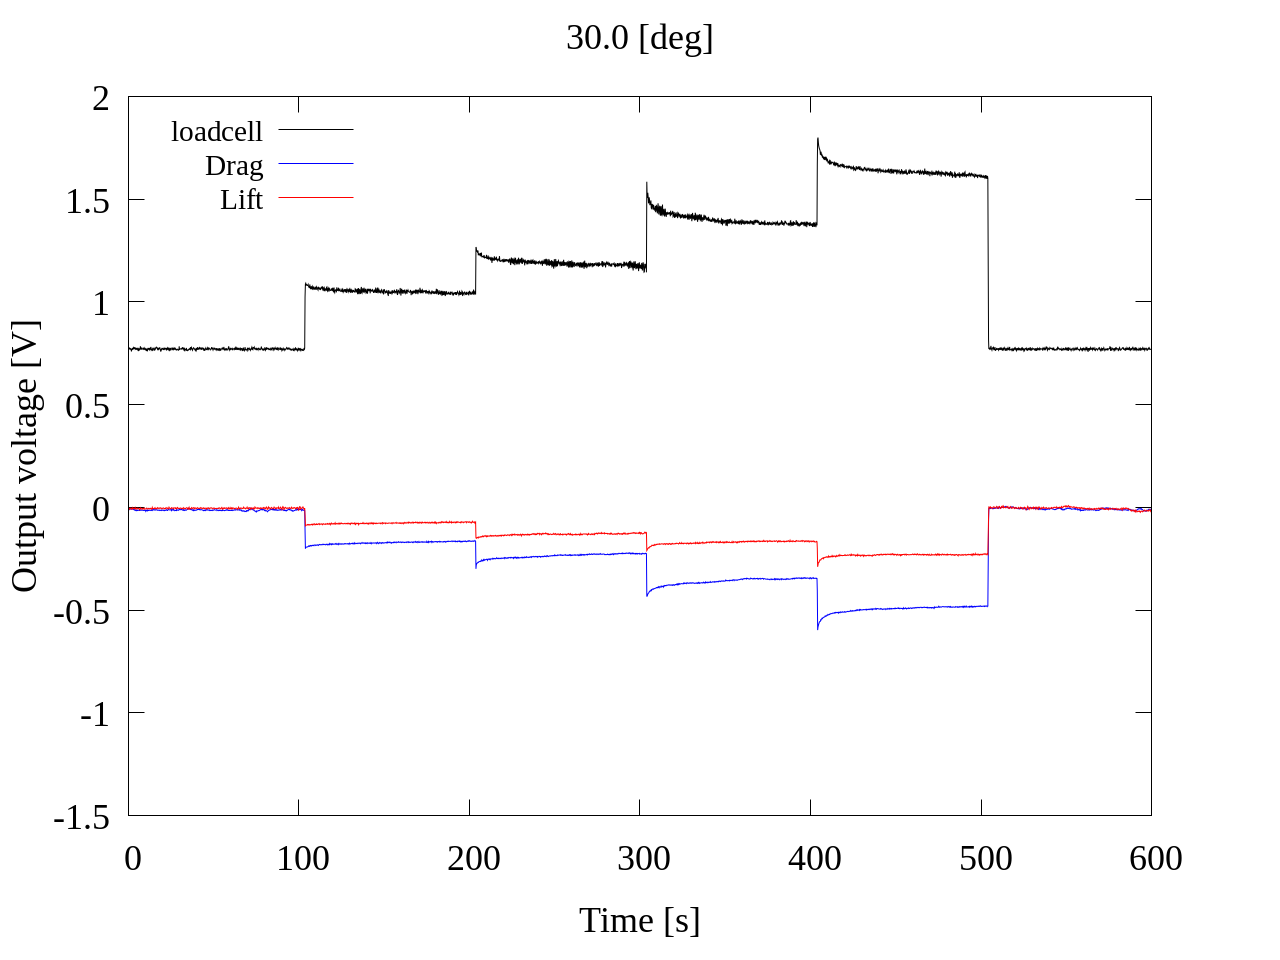
\includegraphics[width=65mm]{../../02_workspace/result/2-1/plot/01-3_allsensors/01_allsensors_300.png}
%         \subcaption{30 [deg]}
%       \end{minipage}
%       \begin{minipage}[b]{0.45\linewidth}
%         \centering
%         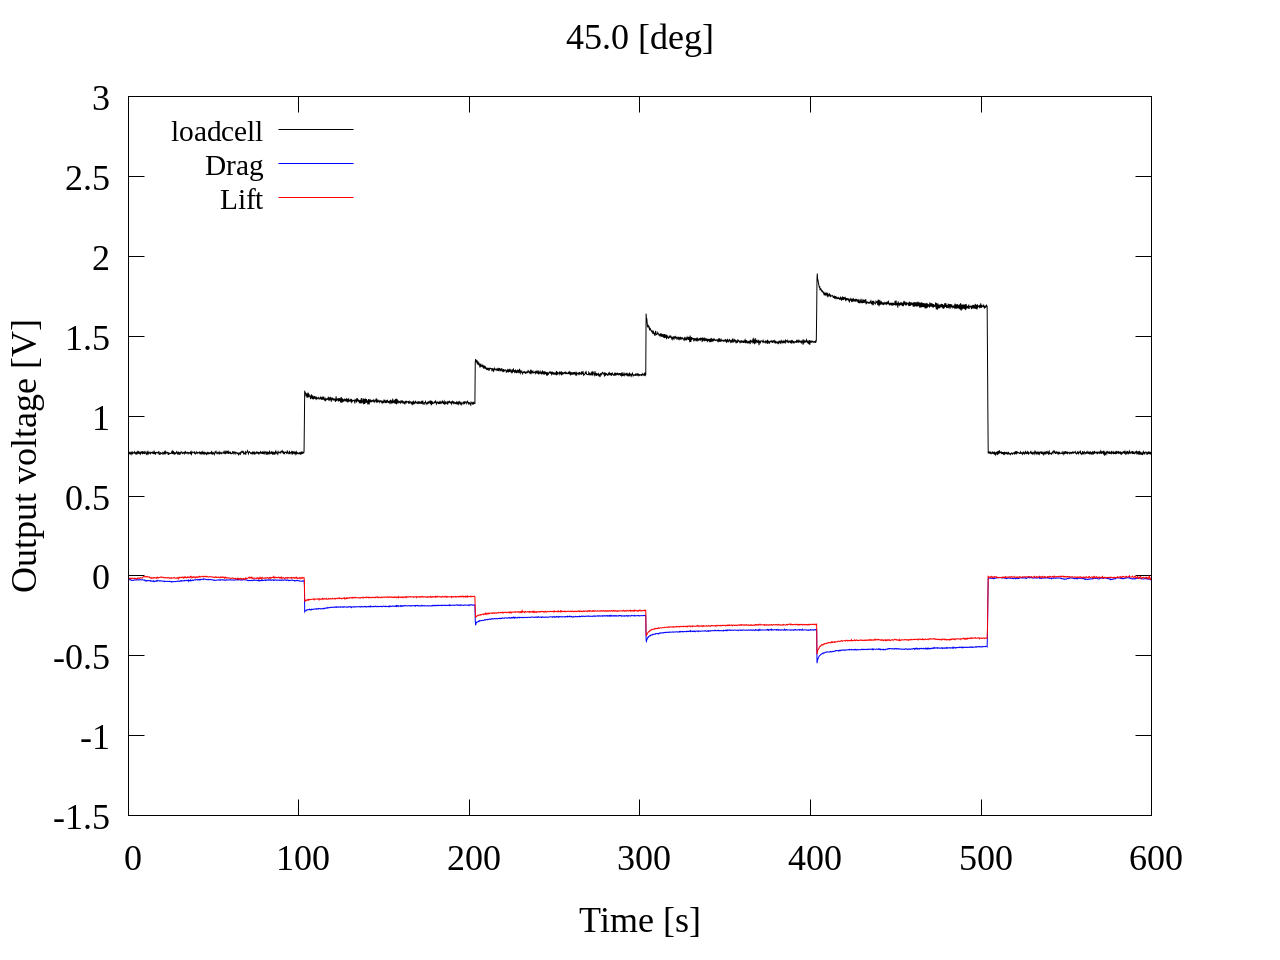
\includegraphics[width=65mm]{../../02_workspace/result/2-1/plot/01-3_allsensors/01_allsensors_450.png}
%         \subcaption{45 [deg]}
%       \end{minipage}\\
%       \begin{minipage}[b]{0.45\linewidth}
%         \centering
%         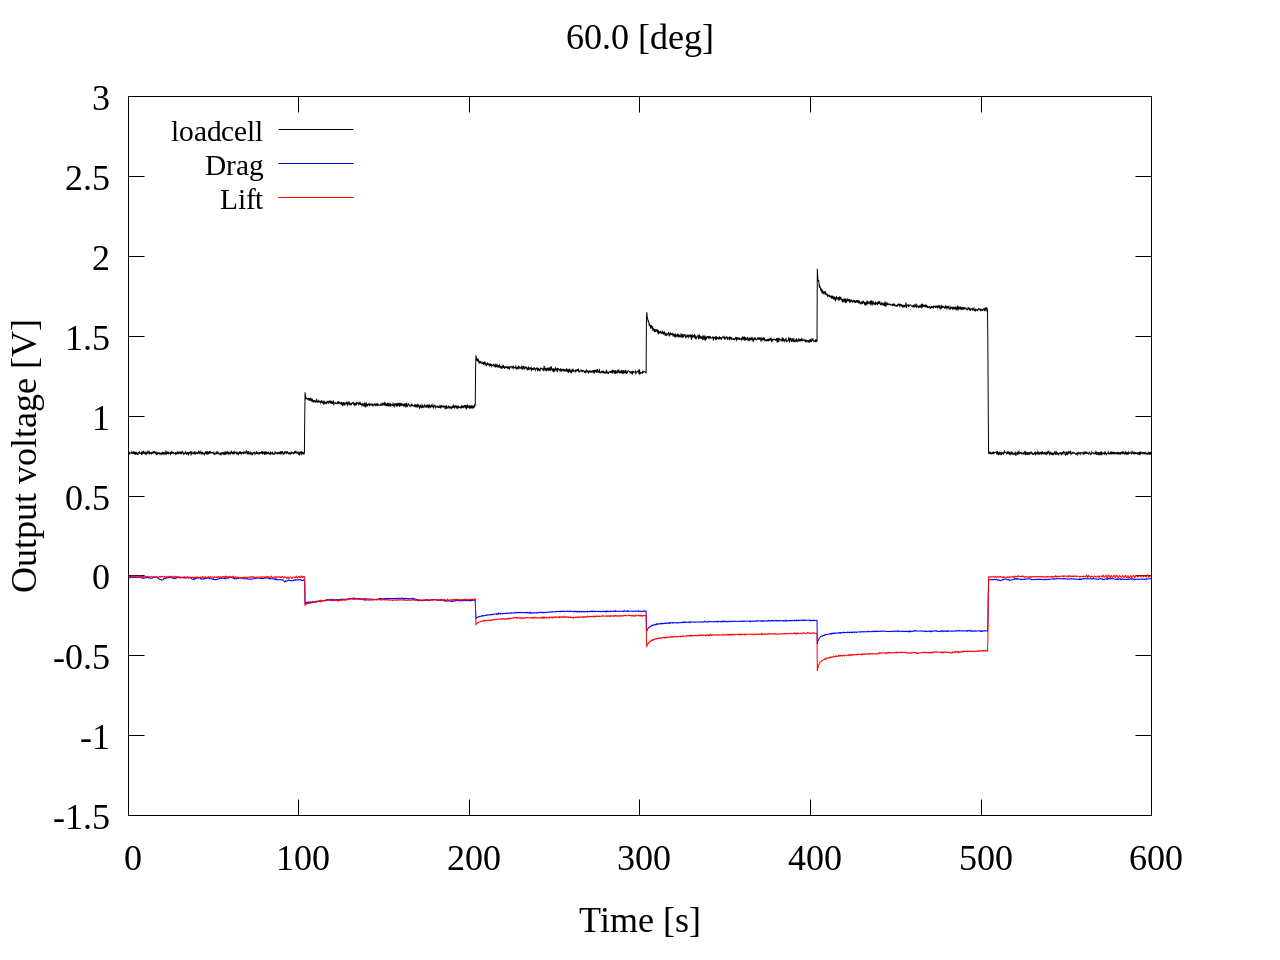
\includegraphics[width=65mm]{../../02_workspace/result/2-1/plot/01-3_allsensors/01_allsensors_600.png}
%         \subcaption{60 [deg]}
%       \end{minipage}
%       \begin{minipage}[b]{0.45\linewidth}
%         \centering
%         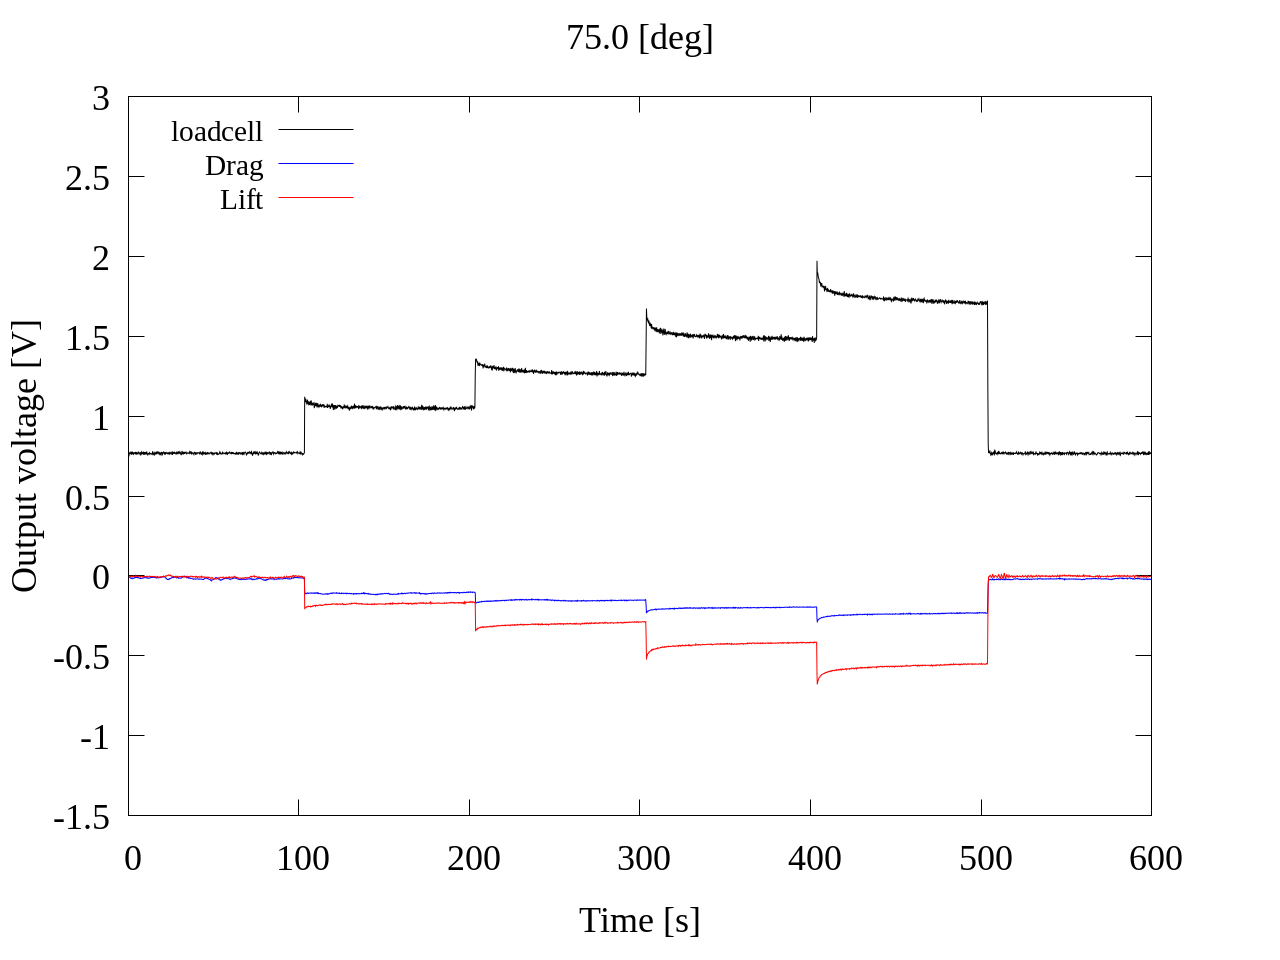
\includegraphics[width=65mm]{../../02_workspace/result/2-1/plot/01-3_allsensors/01_allsensors_750.png}
%         \subcaption{75 [deg]}
%       \end{minipage} 
% \end{figure}

% \begin{figure}[htbp]
%       \begin{minipage}[b]{0.45\linewidth}
%         \centering
%       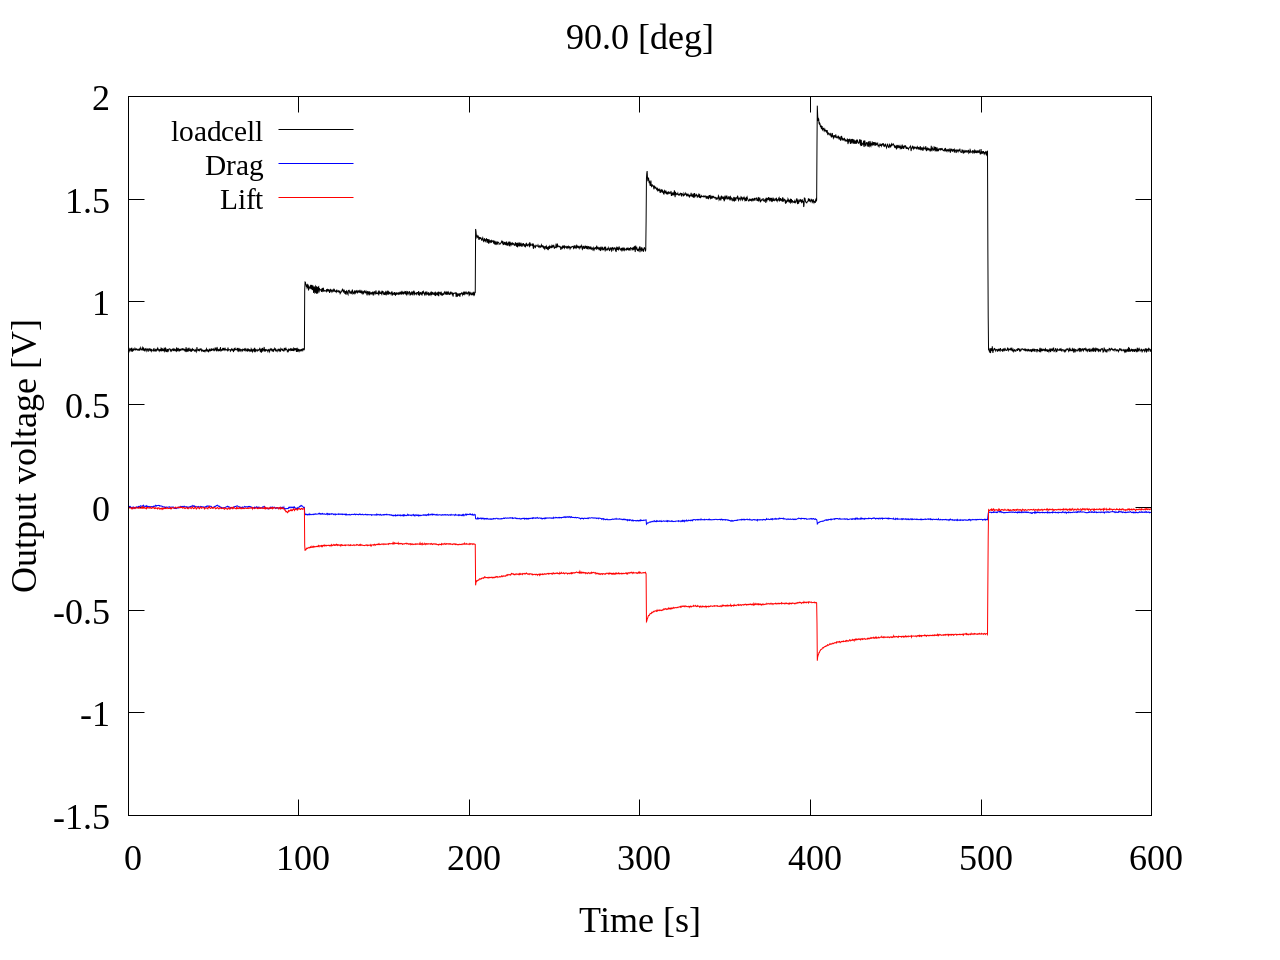
\includegraphics[width=65mm]{../../02_workspace/result/2-1/plot/01-3_allsensors/01_allsensors_900.png}
%       \subcaption{90 [deg]}
%     \end{minipage}
%     \begin{minipage}[b]{0.45\linewidth}
%         \centering
%         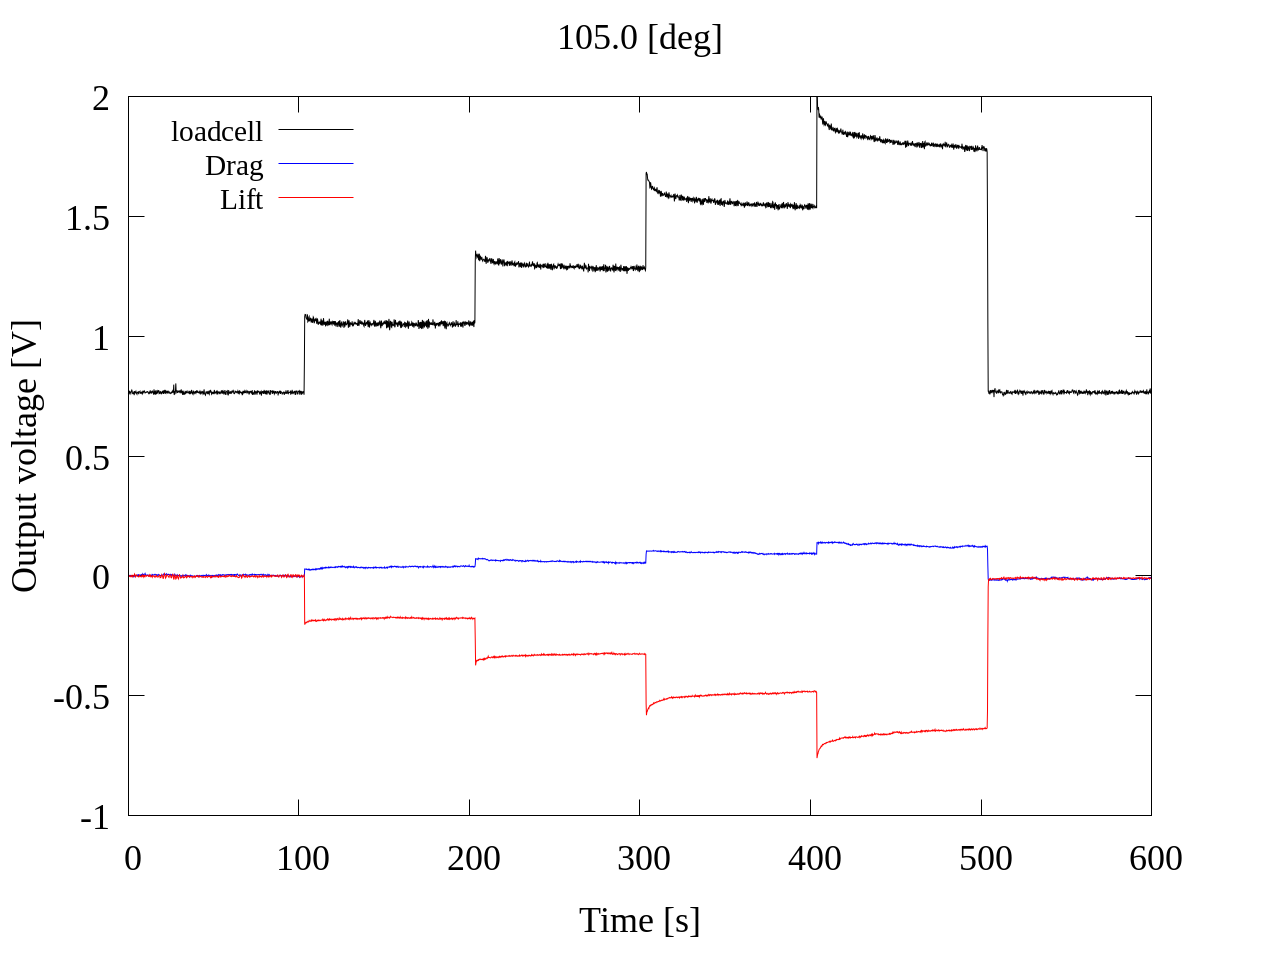
\includegraphics[width=65mm]{../../02_workspace/result/2-1/plot/01-3_allsensors/01_allsensors_1050.png}
%         \subcaption{105 [deg]}
%       \end{minipage}\\
%       \begin{minipage}[b]{0.45\linewidth}
%         \centering
%         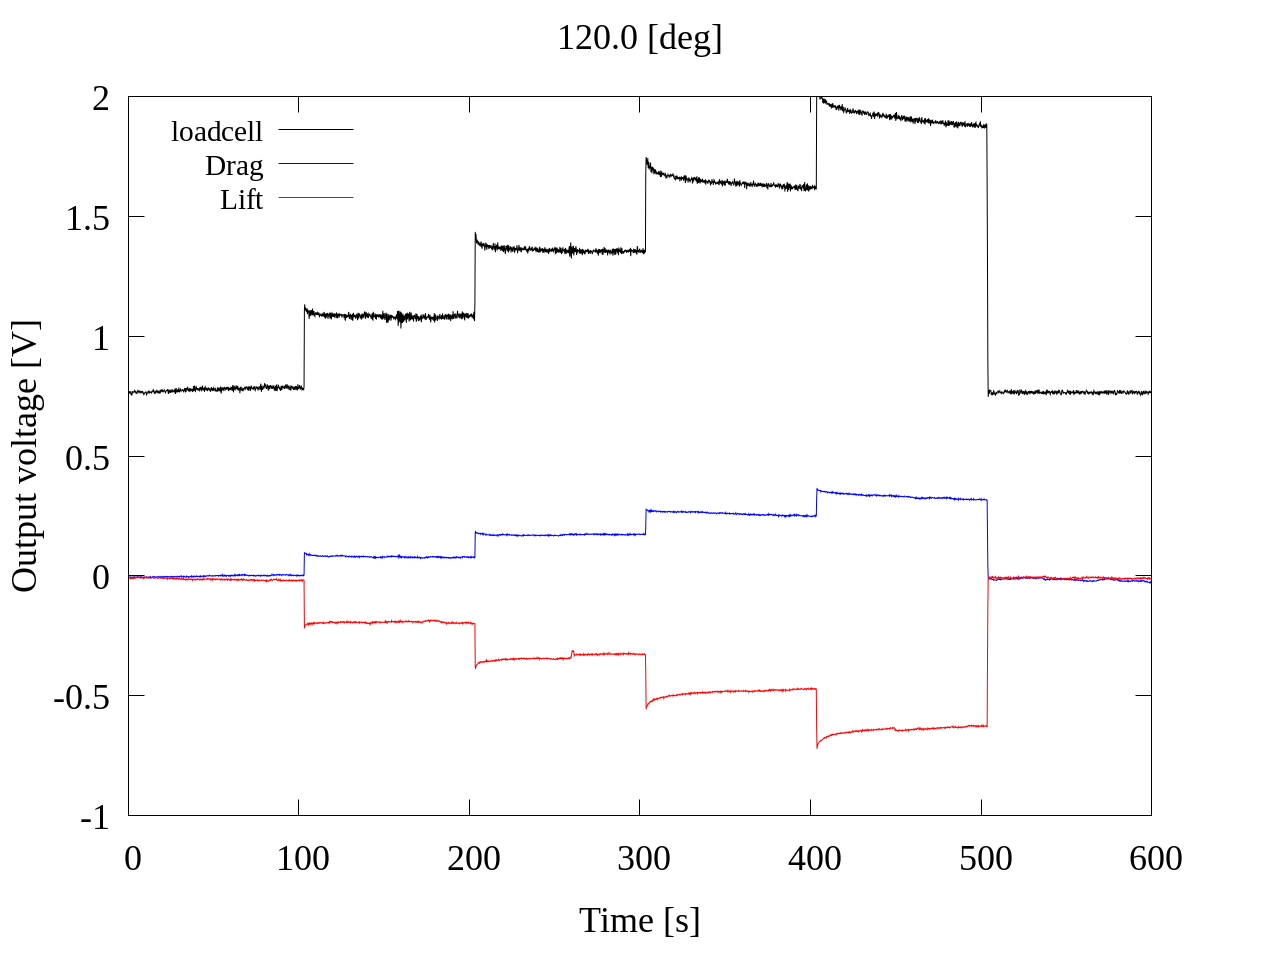
\includegraphics[width=65mm]{../../02_workspace/result/2-1/plot/01-3_allsensors/01_allsensors_1200.png}
%         \subcaption{120 [deg]}
%       \end{minipage}
%       \begin{minipage}[b]{0.45\linewidth}
%         \centering
%         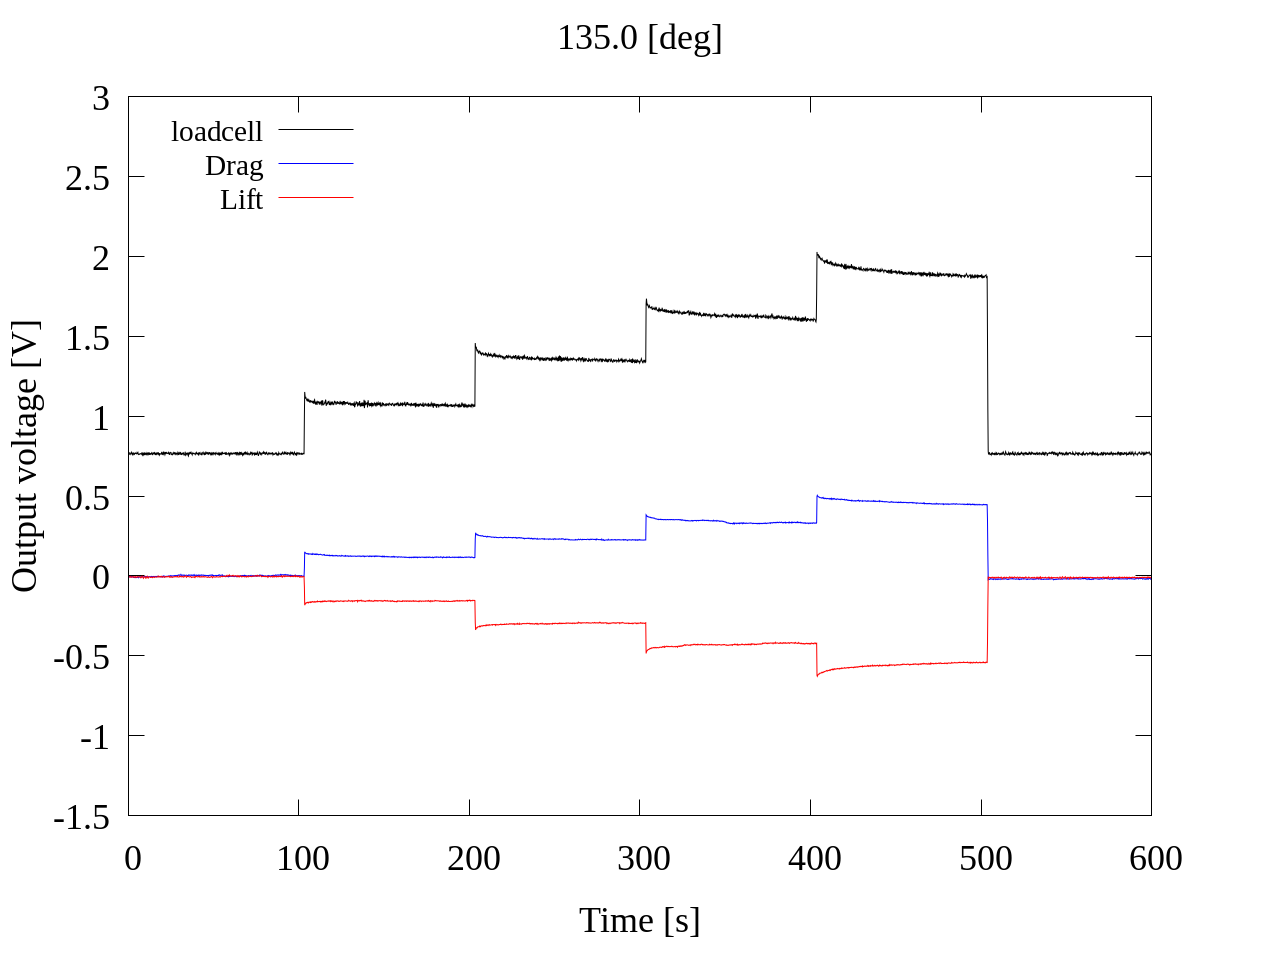
\includegraphics[width=65mm]{../../02_workspace/result/2-1/plot/01-3_allsensors/01_allsensors_1350.png}
%         \subcaption{135 [deg]}
%       \end{minipage}\\
%       \begin{minipage}[b]{0.45\linewidth}
%         \centering
%         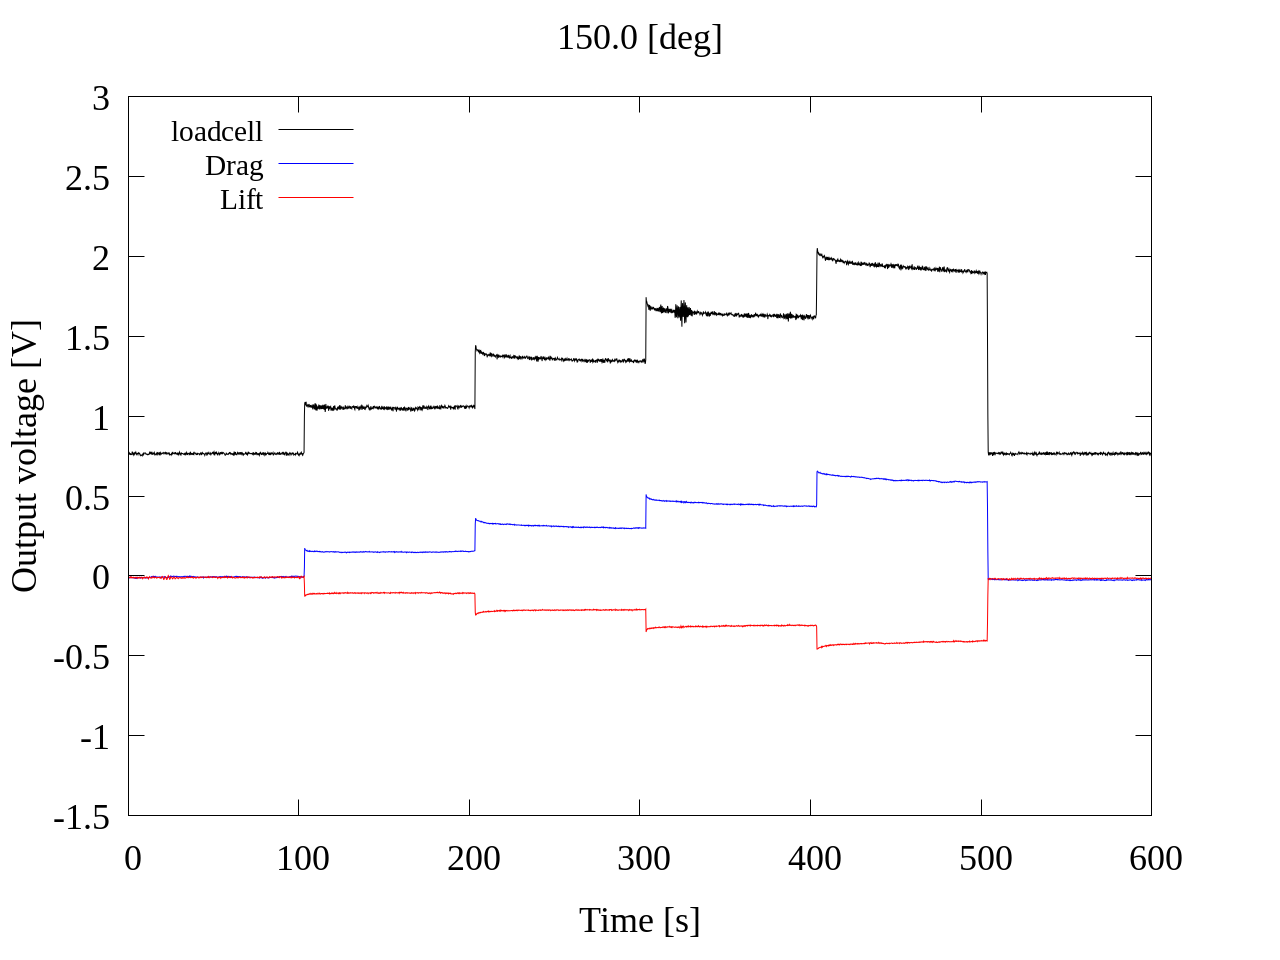
\includegraphics[width=65mm]{../../02_workspace/result/2-1/plot/01-3_allsensors/01_allsensors_1500.png}
%         \subcaption{150 [deg]}
%       \end{minipage} 
%       \begin{minipage}[b]{0.45\linewidth}
%         \centering
%         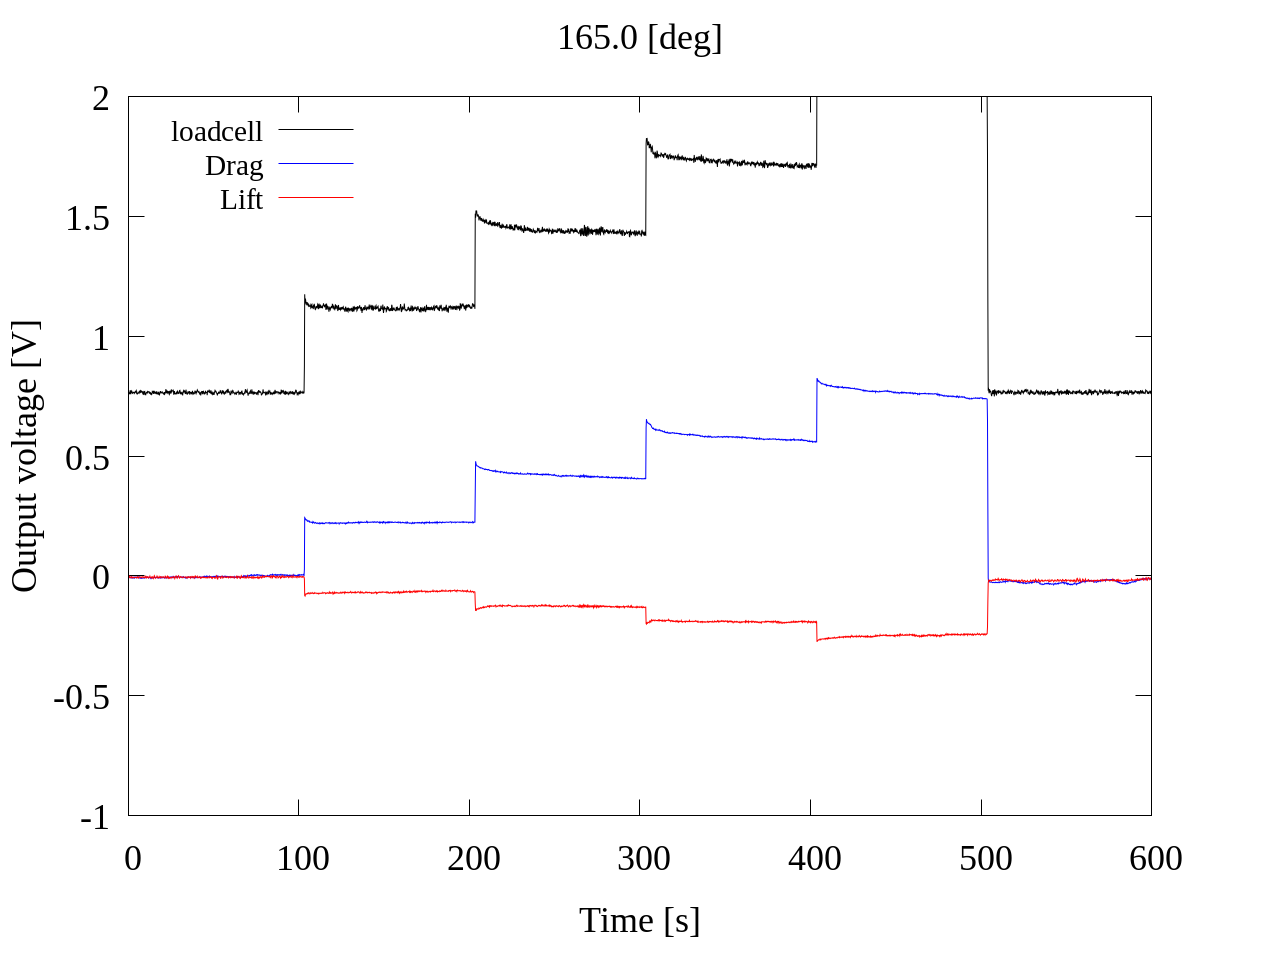
\includegraphics[width=65mm]{../../02_workspace/result/2-1/plot/01-3_allsensors/01_allsensors_1650.png}
%         \subcaption{165 [deg]}
%       \end{minipage}\\
% \end{figure}

% \begin{figure}[htbp]
%       \begin{minipage}[b]{0.45\linewidth}
%         \centering
%         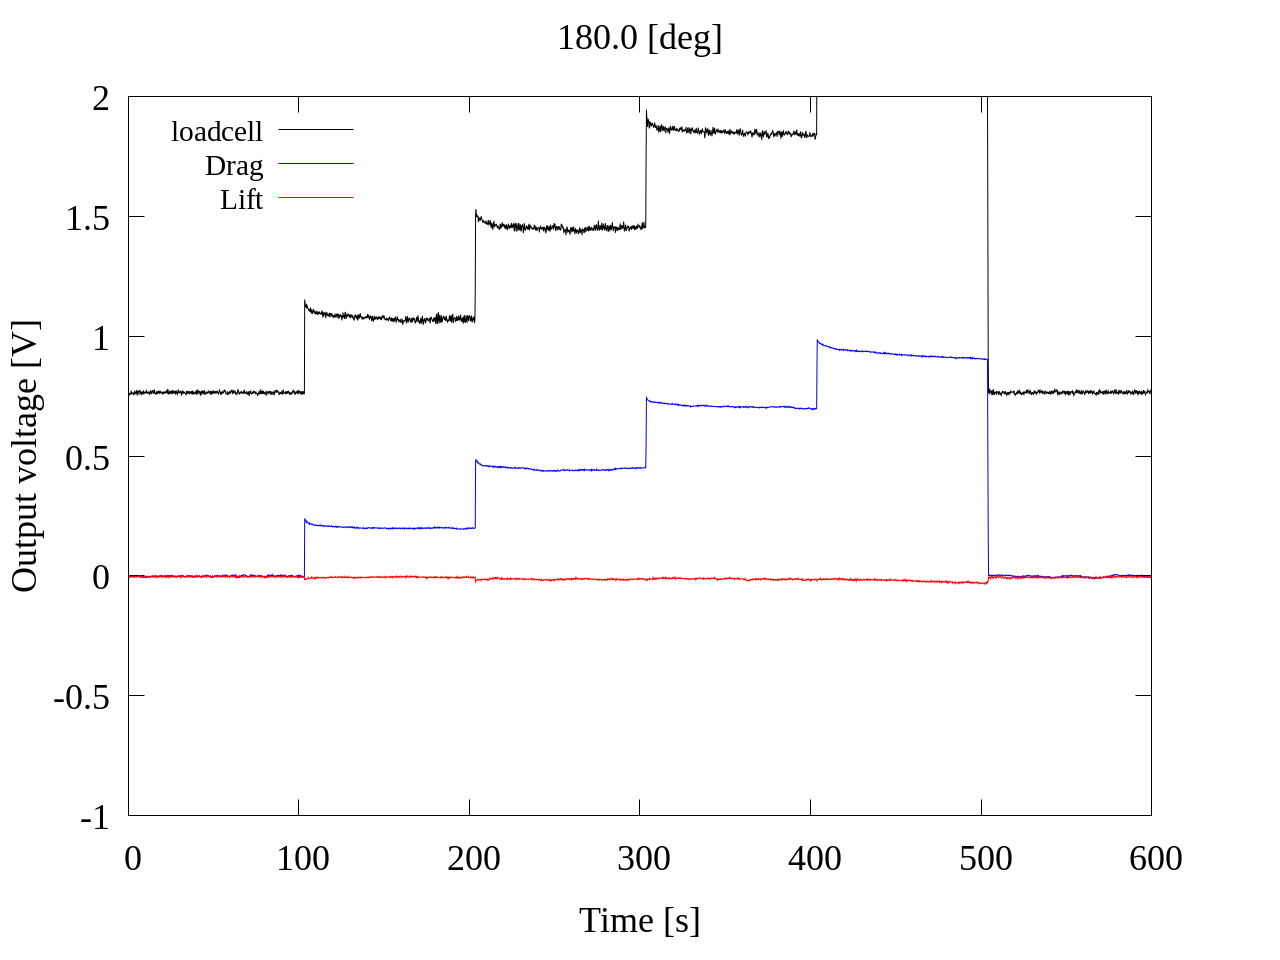
\includegraphics[width=65mm]{../../02_workspace/result/2-1/plot/01-3_allsensors/01_allsensors_1800.png}
%         \subcaption{180 [deg]}
%       \end{minipage}
%       \begin{minipage}[b]{0.45\linewidth}
%         \centering
%         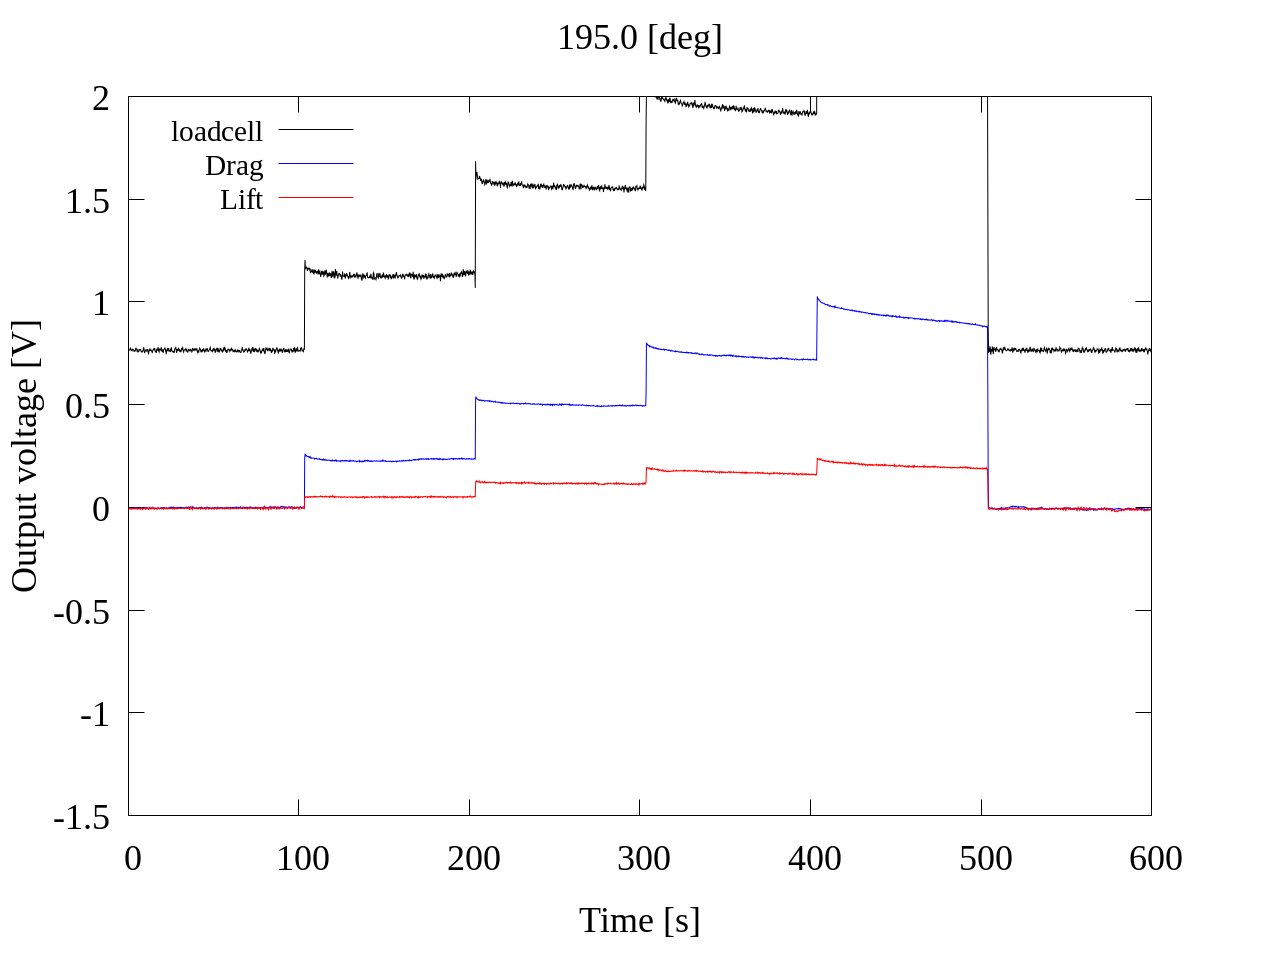
\includegraphics[width=65mm]{../../02_workspace/result/2-1/plot/01-3_allsensors/01_allsensors_1950.png}
%         \subcaption{195 [deg]}
%       \end{minipage}\\

%       \begin{minipage}[b]{0.45\linewidth}
%         \centering
%         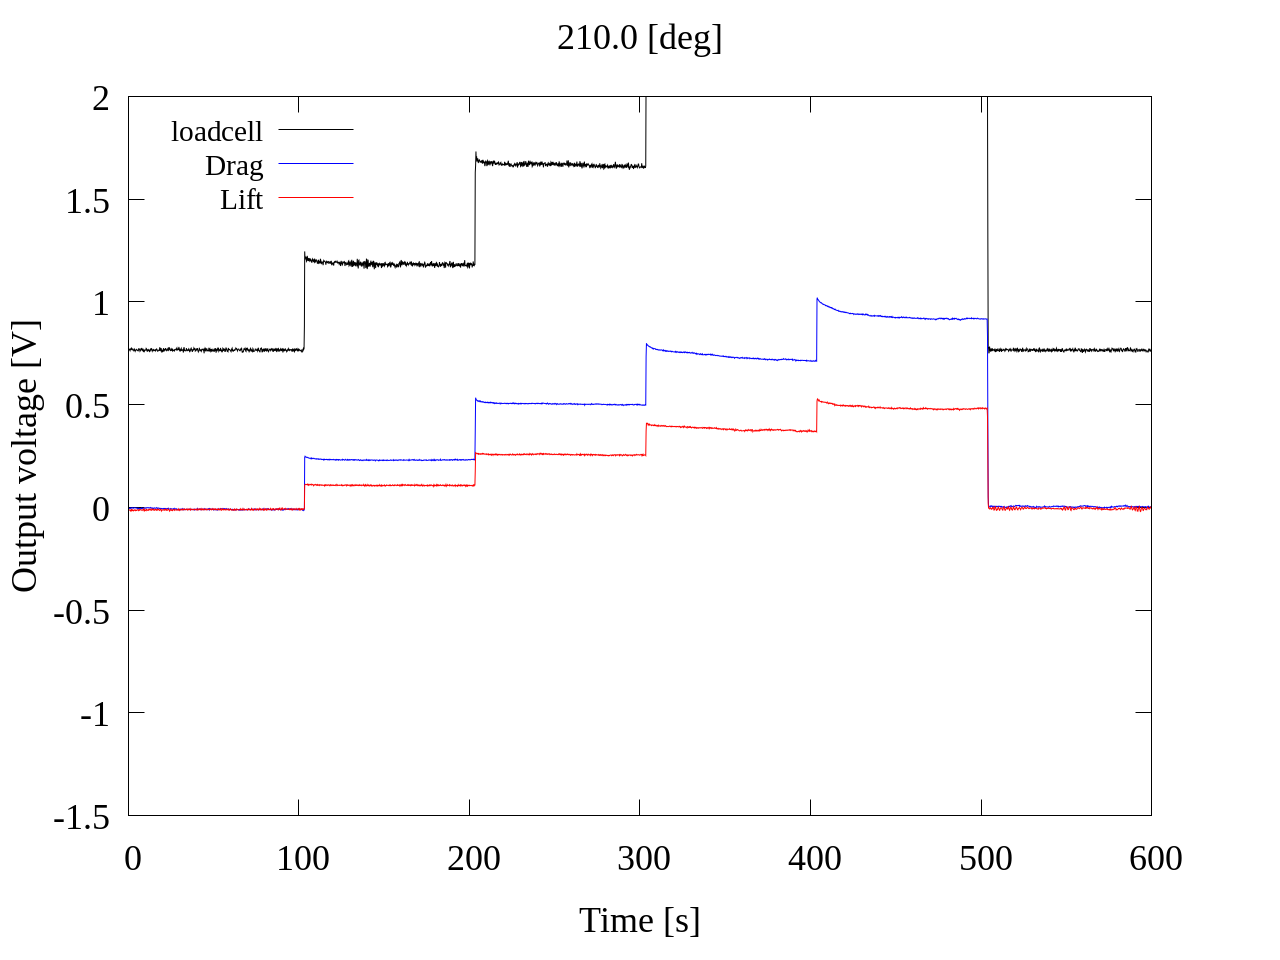
\includegraphics[width=65mm]{../../02_workspace/result/2-1/plot/01-3_allsensors/01_allsensors_2100.png}
%         \subcaption{210 [deg]}
%       \end{minipage}
%       \begin{minipage}[b]{0.45\linewidth}
%         \centering
%         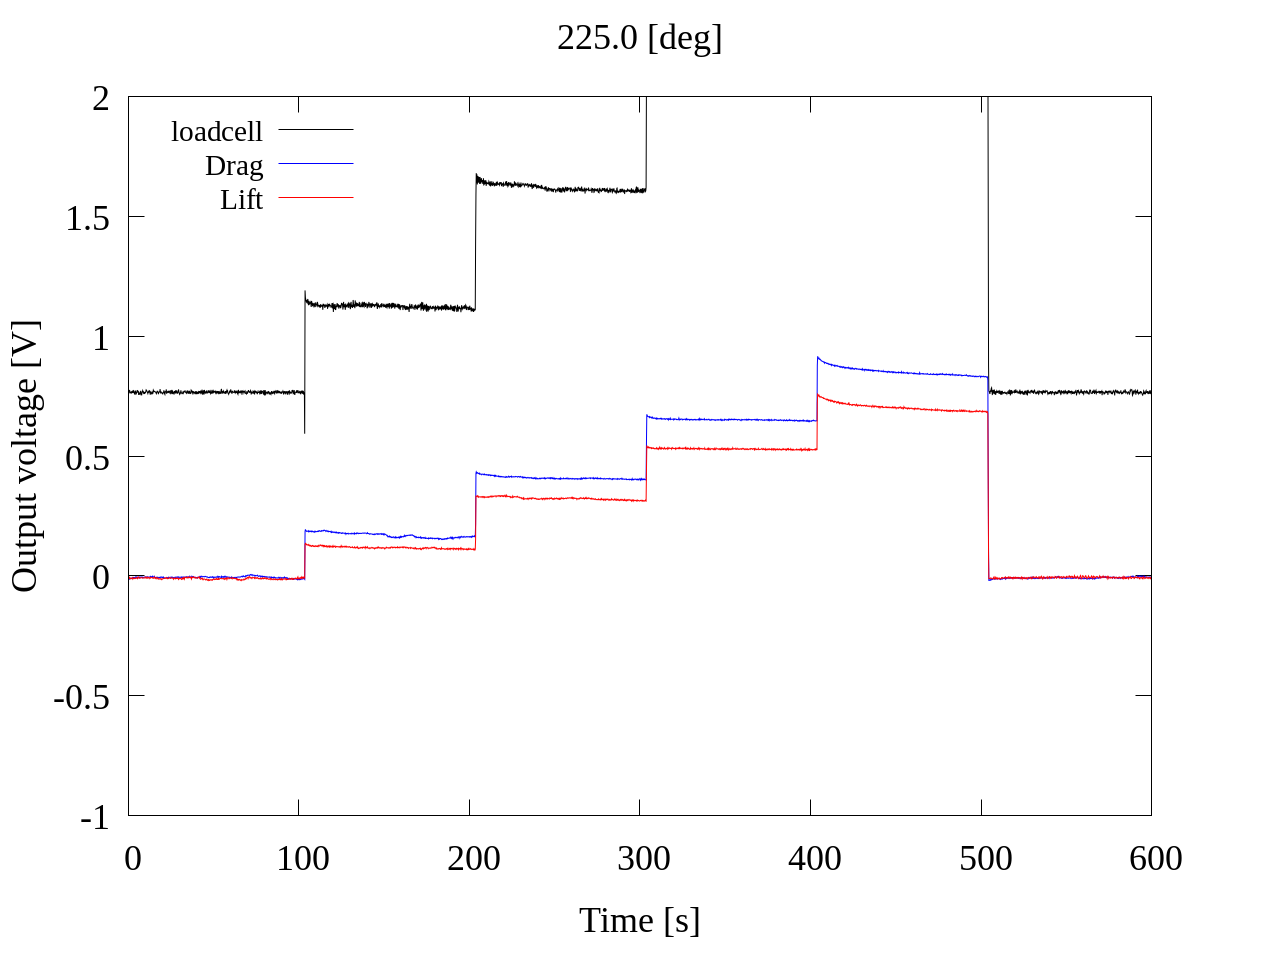
\includegraphics[width=65mm]{../../02_workspace/result/2-1/plot/01-3_allsensors/01_allsensors_2250.png}
%         \subcaption{225 [deg]}
%       \end{minipage}\\

%       \begin{minipage}[b]{0.45\linewidth}
%         \centering
%         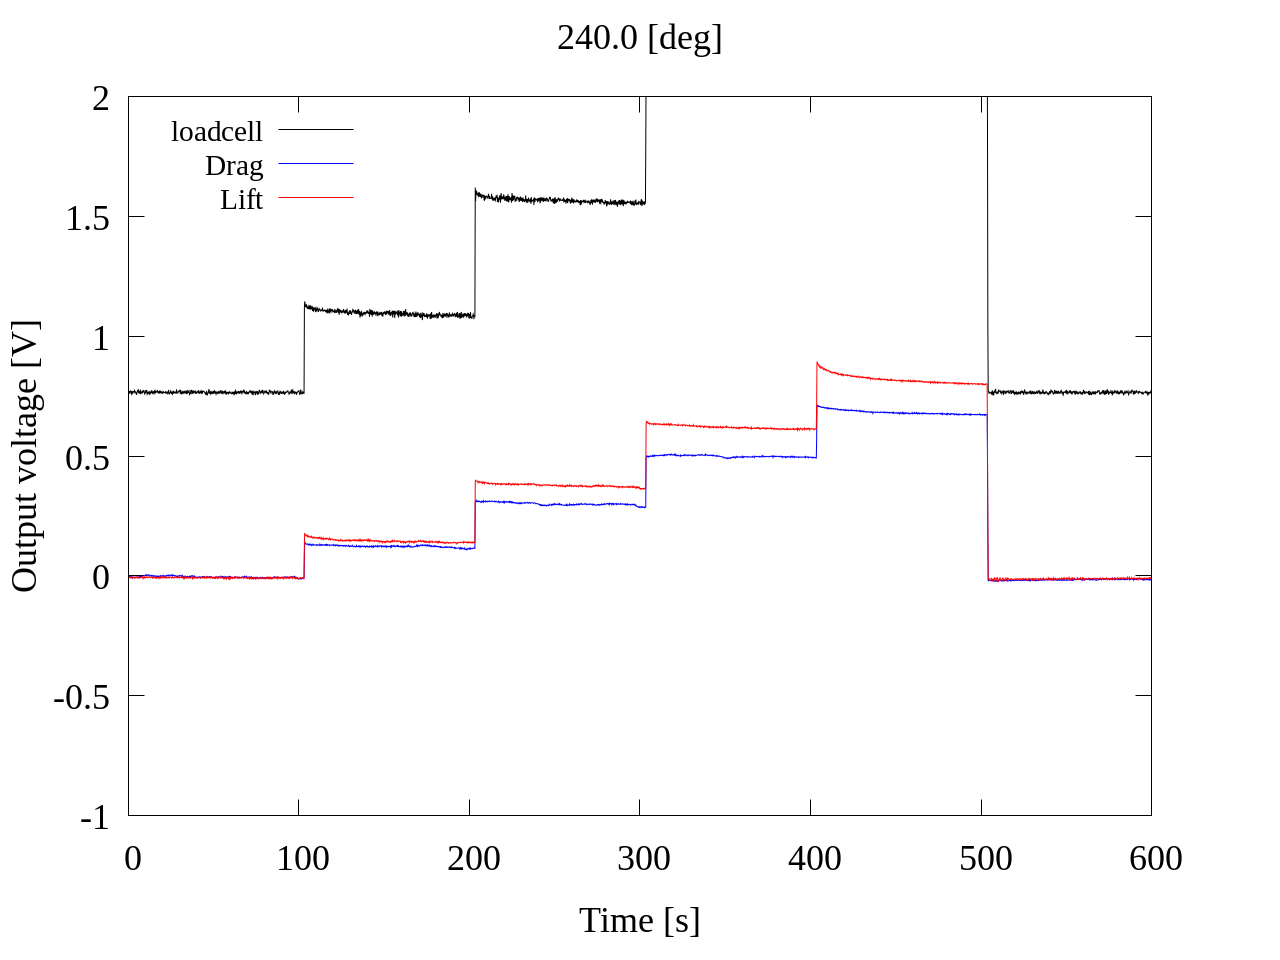
\includegraphics[width=65mm]{../../02_workspace/result/2-1/plot/01-3_allsensors/01_allsensors_2400.png}
%         \subcaption{240 [deg]}
%       \end{minipage}
%       \begin{minipage}[b]{0.45\linewidth}
%         \centering
%         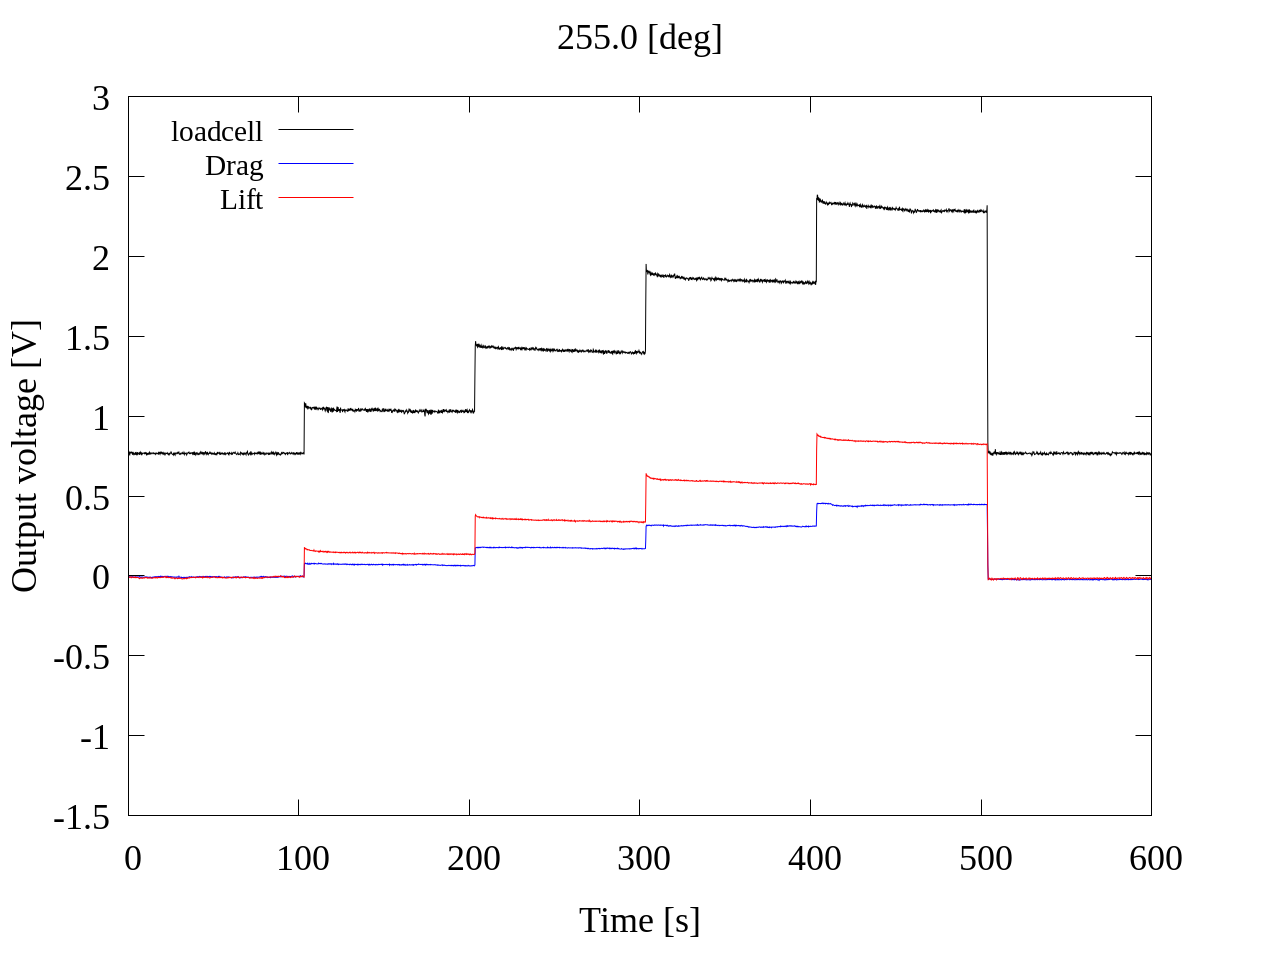
\includegraphics[width=65mm]{../../02_workspace/result/2-1/plot/01-3_allsensors/01_allsensors_2550.png}
%         \subcaption{255 [deg]}
%       \end{minipage}
%     \end{figure}

%     \begin{figure}[htbp]
%       \begin{minipage}[b]{0.45\linewidth}
%         \centering
%         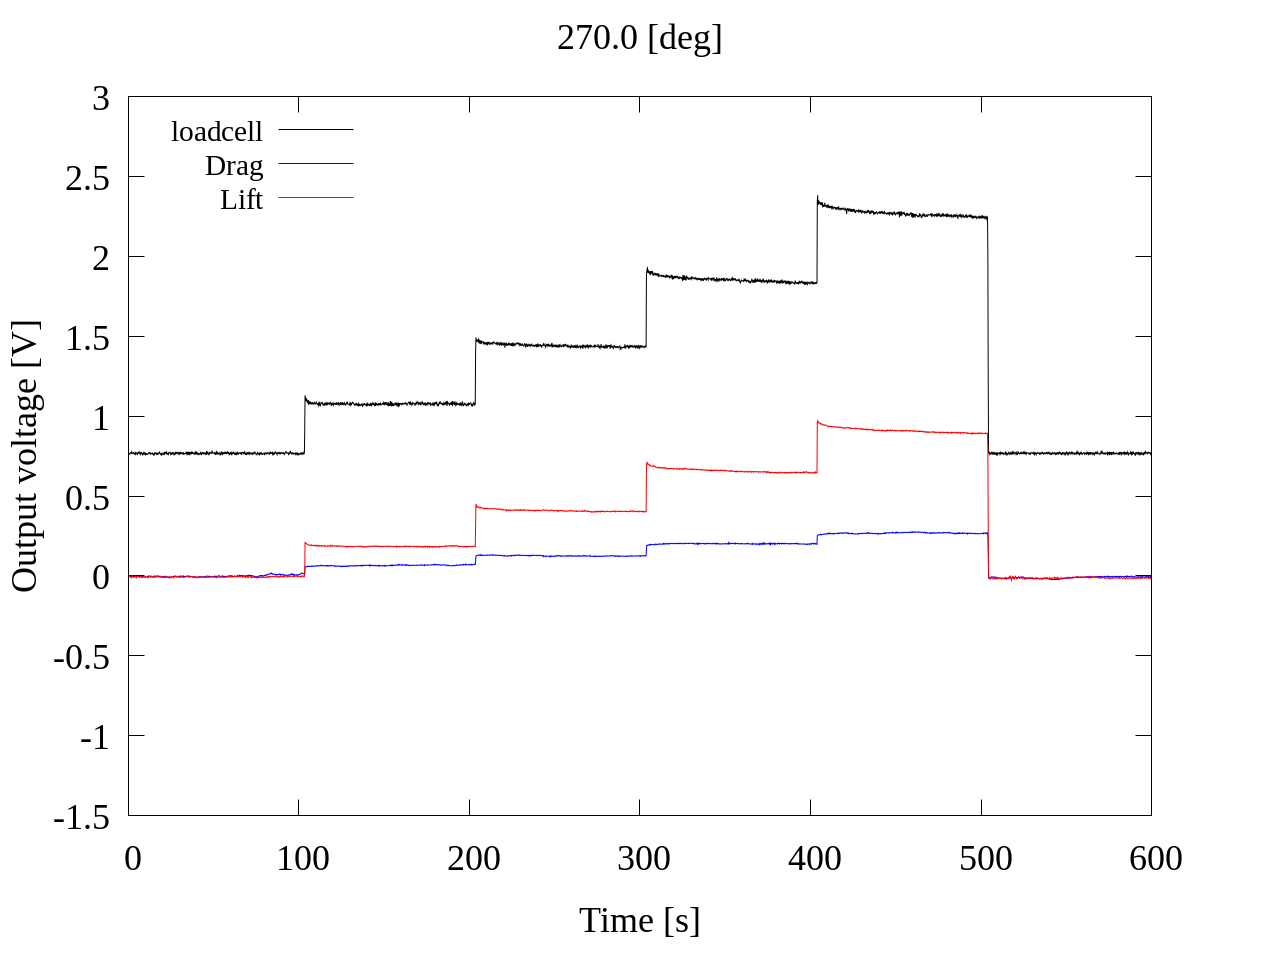
\includegraphics[width=65mm]{../../02_workspace/result/2-1/plot/01-3_allsensors/01_allsensors_2700.png}
%         \subcaption{270 [deg]}
%       \end{minipage}
%       \begin{minipage}[b]{0.45\linewidth}
%         \centering
%         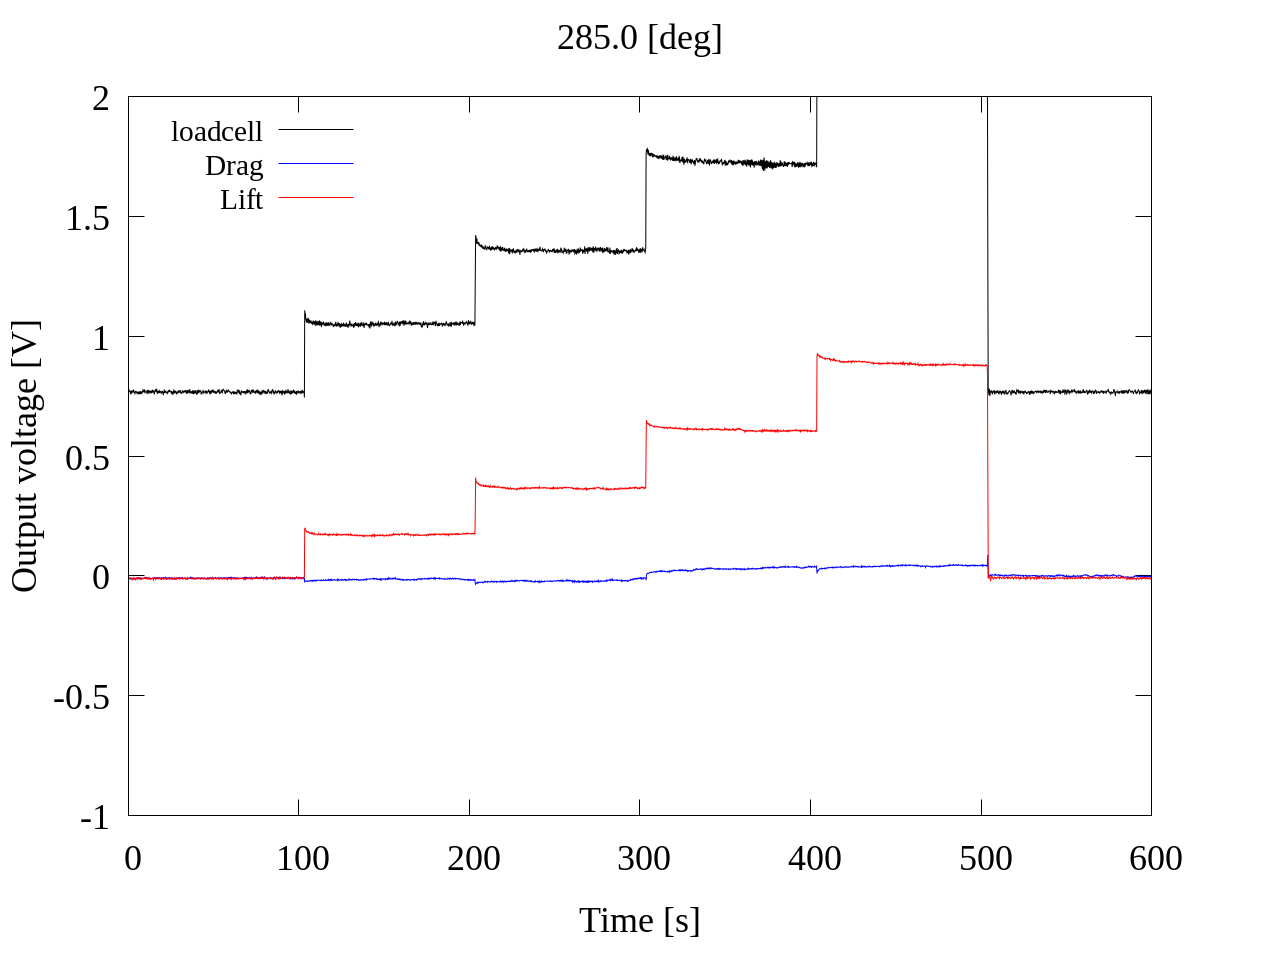
\includegraphics[width=65mm]{../../02_workspace/result/2-1/plot/01-3_allsensors/01_allsensors_2850.png}
%         \subcaption{285 [deg]}
%       \end{minipage}\\

%       \begin{minipage}[b]{0.45\linewidth}
%         \centering
%         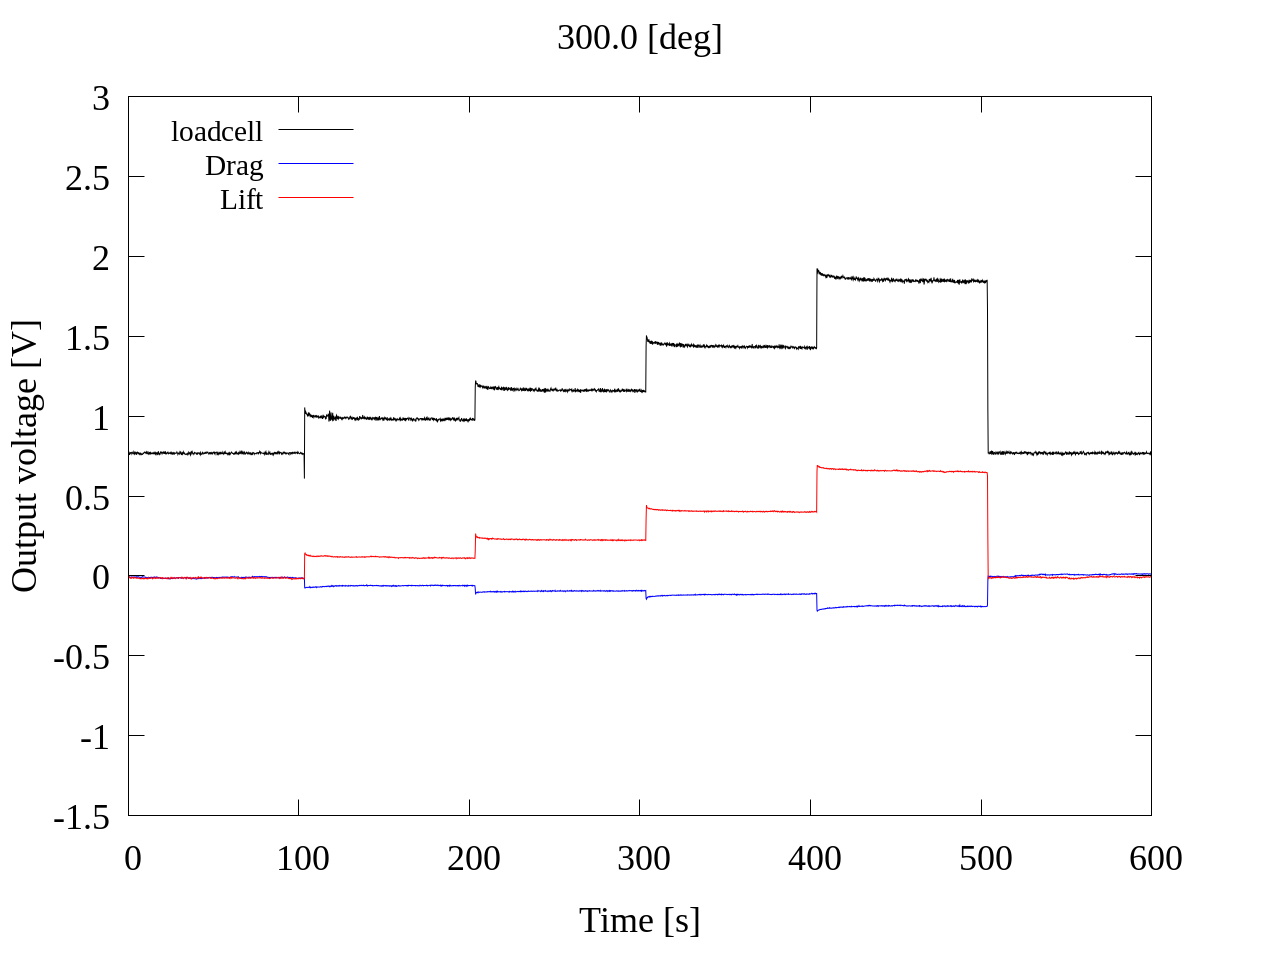
\includegraphics[width=65mm]{../../02_workspace/result/2-1/plot/01-3_allsensors/01_allsensors_3000.png}
%         \subcaption{300 [deg]}
%       \end{minipage}
%       \begin{minipage}[b]{0.45\linewidth}
%         \centering
%         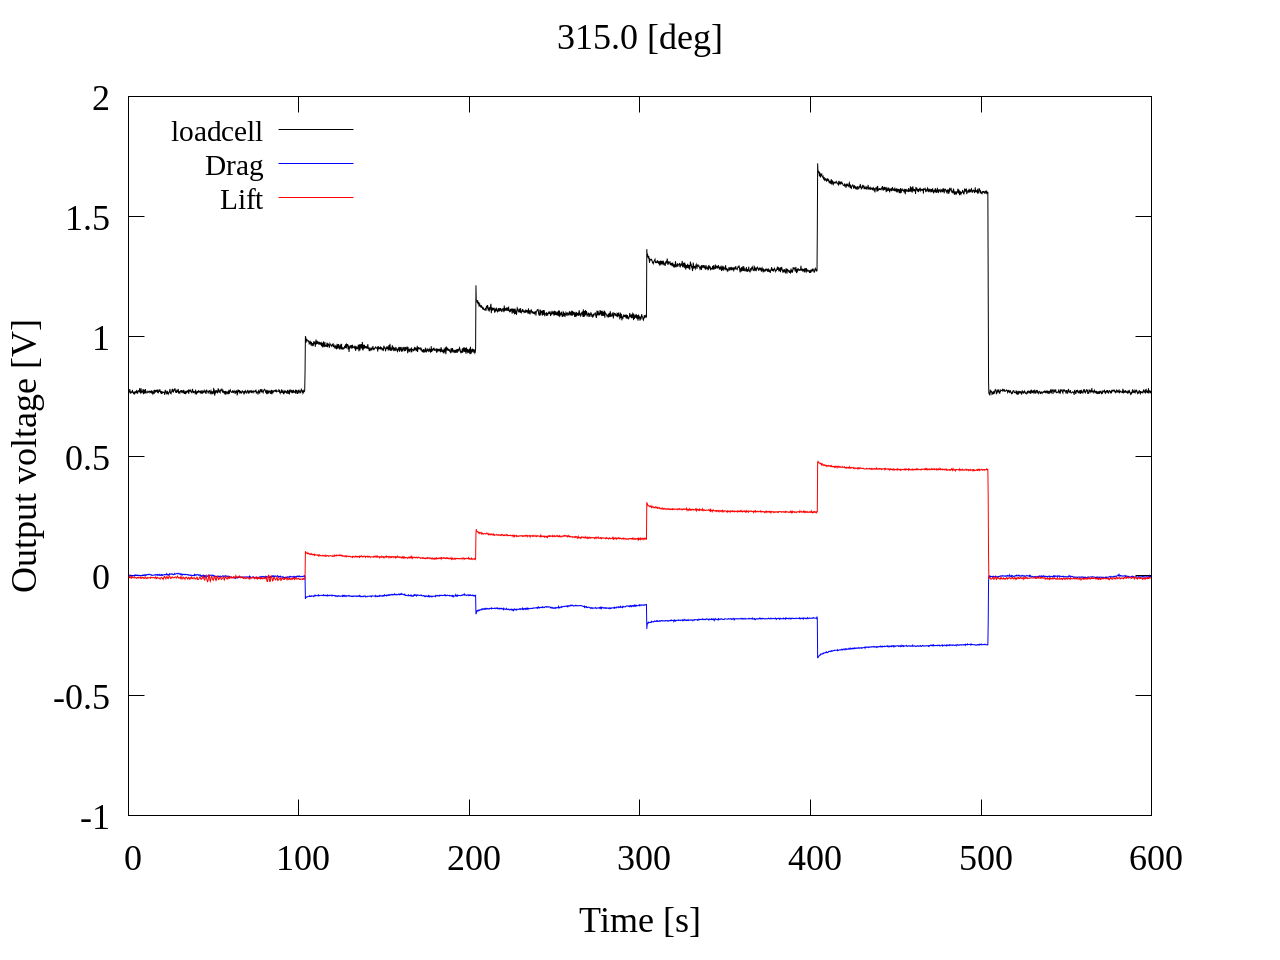
\includegraphics[width=65mm]{../../02_workspace/result/2-1/plot/01-3_allsensors/01_allsensors_3150.png}
%         \subcaption{315 [deg]}
%       \end{minipage}\\

%       \begin{minipage}[b]{0.45\linewidth}
%         \centering
%         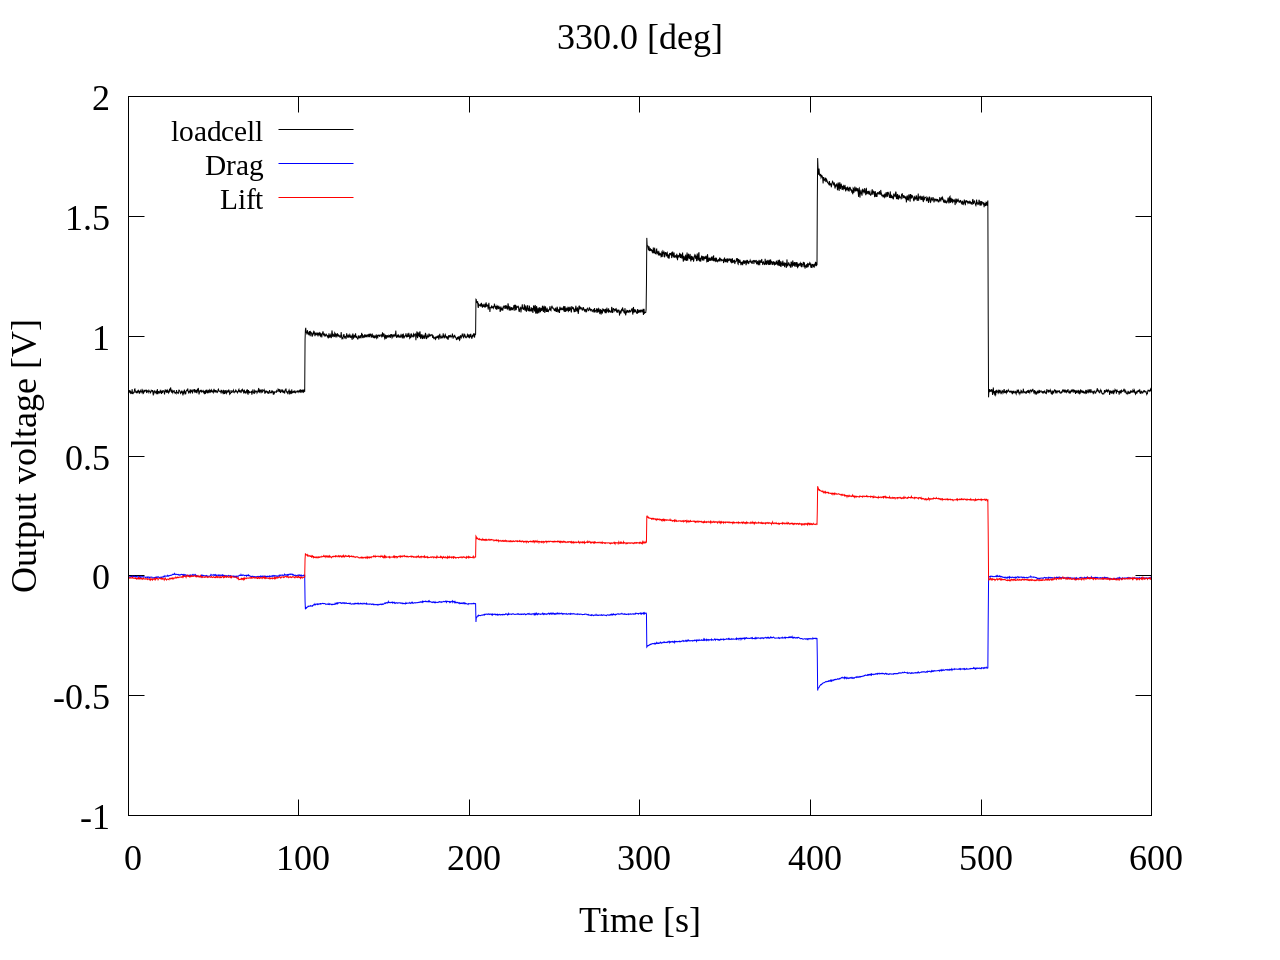
\includegraphics[width=65mm]{../../02_workspace/result/2-1/plot/01-3_allsensors/01_allsensors_3300.png}
%         \subcaption{330 [deg]}
%       \end{minipage}
%       \begin{minipage}[b]{0.45\linewidth}
%         \centering
%         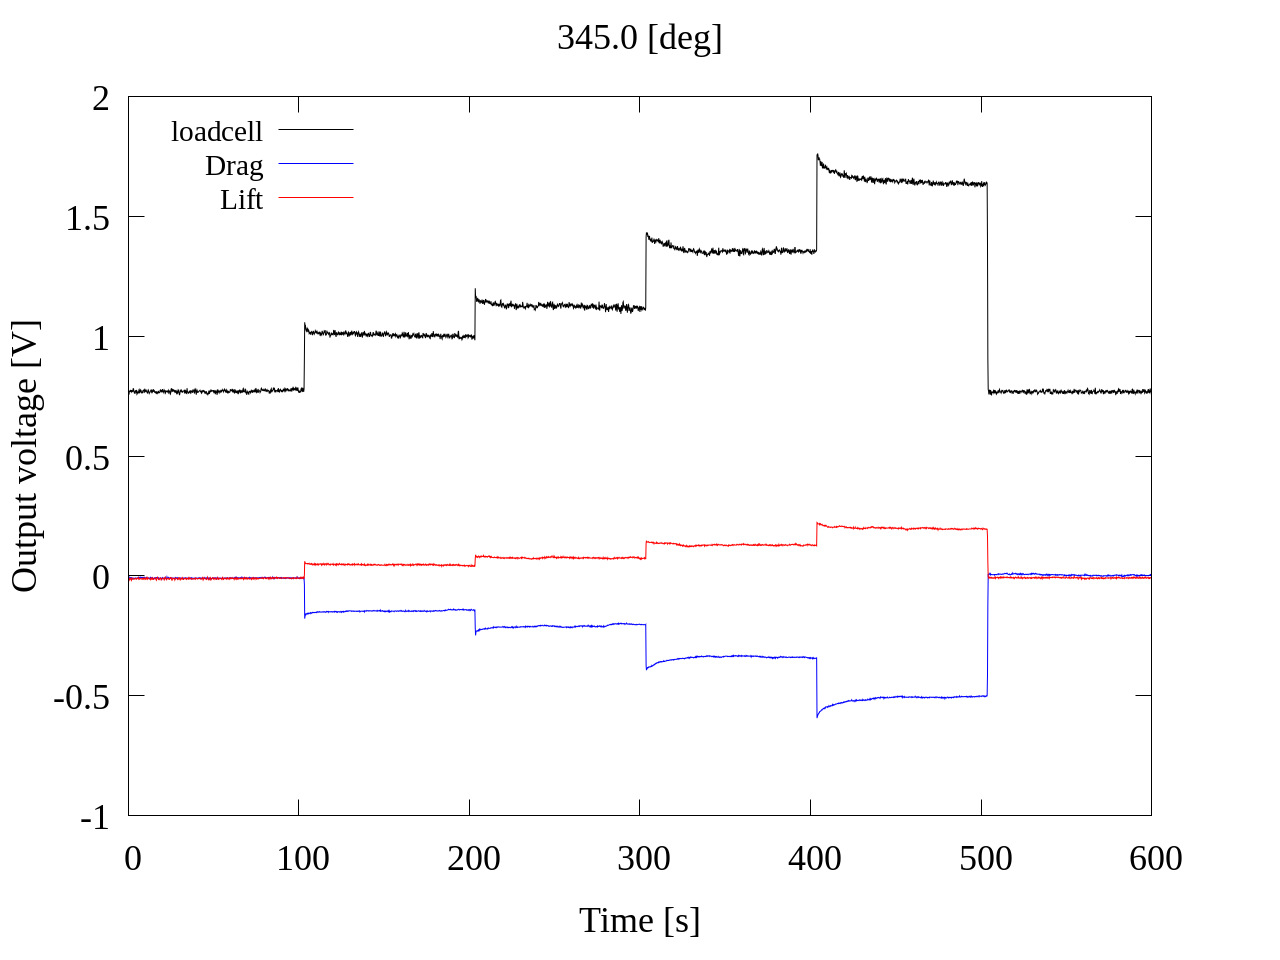
\includegraphics[width=65mm]{../../02_workspace/result/2-1/plot/01-3_allsensors/01_allsensors_3450.png}
%         \subcaption{345 [deg]}
%       \end{minipage}
% \end{figure}

\newpage

以上の結果から自動一軸ステージが移動した直後から出力電圧の減衰がみられる場合があるが,
同様の変化がロードセルおよびひずみセンサにみられることから大きな問題はないと考える.

\subsection{データ処理手法}

実験結果から,式()の出力電圧勾配を算出する.
そのために以下の手順でデータ処理を行った.

\begin{enumerate}[(1)]
	\item ドリフト補正
	\item 各距離における平均値の算出
	\item 出力電圧勾配の算出
\end{enumerate}

ここで,例として 1回目の性能評価実験,0 [deg]におけるロードセルの出力電圧の図 (Fig.) を用いて説明する.\\
※ ロードセルの出力電圧は使用しているストレインアンプの影響によりオフセット値を持つ.

\begin{figure}[htbp]
	\footnotesize
	\begin{center}
		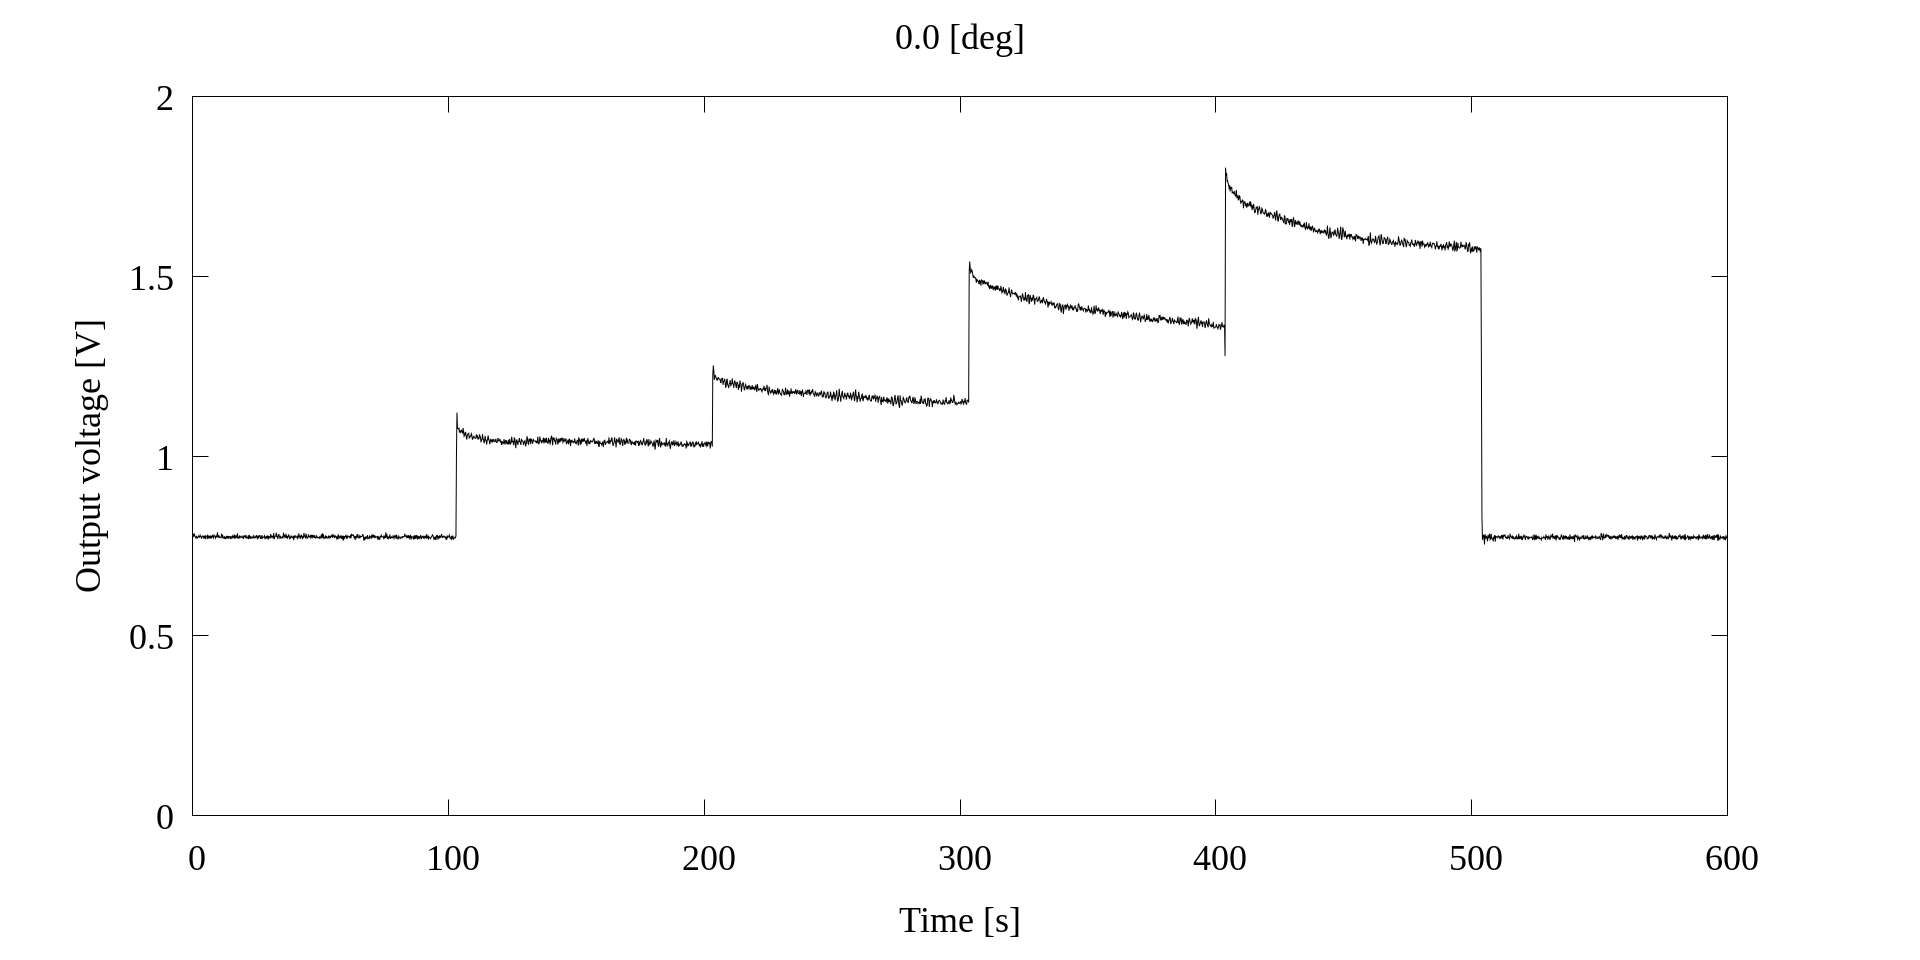
\includegraphics[width=95mm]{../../02_workspace/result/2-1/plot/01-1_loadcell/01_loadcell_0.png}
		\caption{Loadcell output voltage : 0 [deg]}
	\end{center}
\end{figure}

また,このとき実験結果をロードセルの押込距離および時間経過によって
それぞれのデータ範囲についてその呼称を以下のTable のように定義することとする.

\begin{table}[htbp]
	\begin{center}
		\caption{Definition of data name}
		\begin{tabular}{|p{20mm}|p{20mm}|p{20mm}|}
			\hline
			\multicolumn{1}{|c|}{\textgt{Data name}} & \multicolumn{1}{|c|}{\textgt{Pushing length [mm]}} & \multicolumn{1}{|c|}{\textgt{Time [s]}} \\ \hline
			\multicolumn{1}{|c|}{Range : 1}          & \multicolumn{1}{|c|}{0.00}                         & \multicolumn{1}{|c|}{0 $\sim$ 100}      \\ \hline
			\multicolumn{1}{|c|}{Range : 2}          & \multicolumn{1}{|c|}{0.03}                         & \multicolumn{1}{|c|}{100 $\sim$ 200}    \\ \hline
			\multicolumn{1}{|c|}{Range : 3}          & \multicolumn{1}{|c|}{0.06}                         & \multicolumn{1}{|c|}{200 $\sim$ 300}    \\ \hline
			\multicolumn{1}{|c|}{Range : 4}          & \multicolumn{1}{|c|}{0.09}                         & \multicolumn{1}{|c|}{300 $\sim$ 400}    \\ \hline
			\multicolumn{1}{|c|}{Range : 5}          & \multicolumn{1}{|c|}{0.12}                         & \multicolumn{1}{|c|}{400 $\sim$ 500}    \\ \hline
			\multicolumn{1}{|c|}{Range : 6}          & \multicolumn{1}{|c|}{0.00}                         & \multicolumn{1}{|c|}{500 $\sim$ 600}    \\ \hline
		\end{tabular}
	\end{center}
\end{table}

\newpage

\subsubsection{ドリフト補正}
性能評価実験は各角度に対して約10分間の測定を行うが,
ストレインアンプは時間経過に対して基準の電圧が変動する場合がある.
この現象をドリフトと呼ぶ.
そのため,実験結果を出力電圧勾配の算出に用いる
前処理として,ドリフトを考慮したデータへと変換する必要がある.

このとき,以下の手順でドリフト補正を行うこととする.

\begin{enumerate}[(1)]
	\item 測定開始直後(Range : 1)及び終了直前(Range : 6)のデータ(30秒/150点)における平均値を算出
	\item 算出した2つの平均値を結び,直線を作成
	\item 元データと直線の差をとり,補正値として採用する
\end{enumerate}

以下のFig. にドリフト補正を適用した結果を示す.

\begin{figure}[htbp]
	\footnotesize
	\begin{center}
		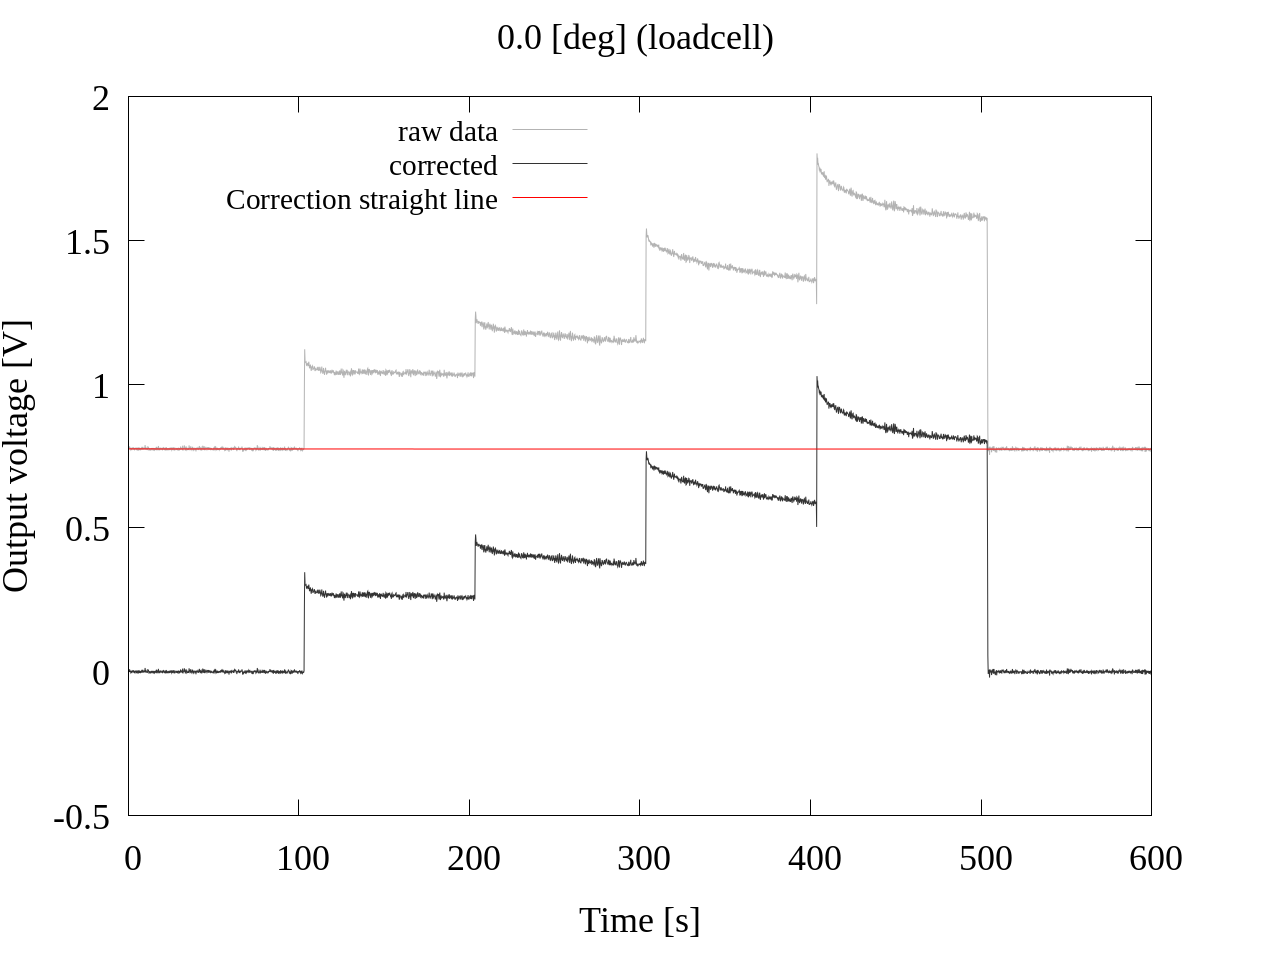
\includegraphics[width=95mm]{../../02_workspace/result/2-1/plot/02-1_loadcell/02_loadcell-drift_0.png}
		\caption{Drift corrected voltage (load cell) : 0 [deg]}
	\end{center}
\end{figure}

Fig.から補正前のデータから算出された補正直線(赤線)の差を取ると
補正後のデータはオフセット値の分だけ移動しており,
タイヤモデルと接触していないとき($t = 0 \sim 100 \; [\mathrm{s}]$,$t = 500 \sim 600 \; [\mathrm{s}]$)の
出力電圧の値は0付近を推移していることがわかる.
したがって,ドリフト補正処理は正しく動作していると考えられる.

また,以下のFig.に抗力及び揚力方向のひずみセンサの出力電圧について
同様のプログラムを用いてドリフト補正処理を行った結果を示す.

\begin{figure}[htbp]
	\footnotesize
	\begin{center}
		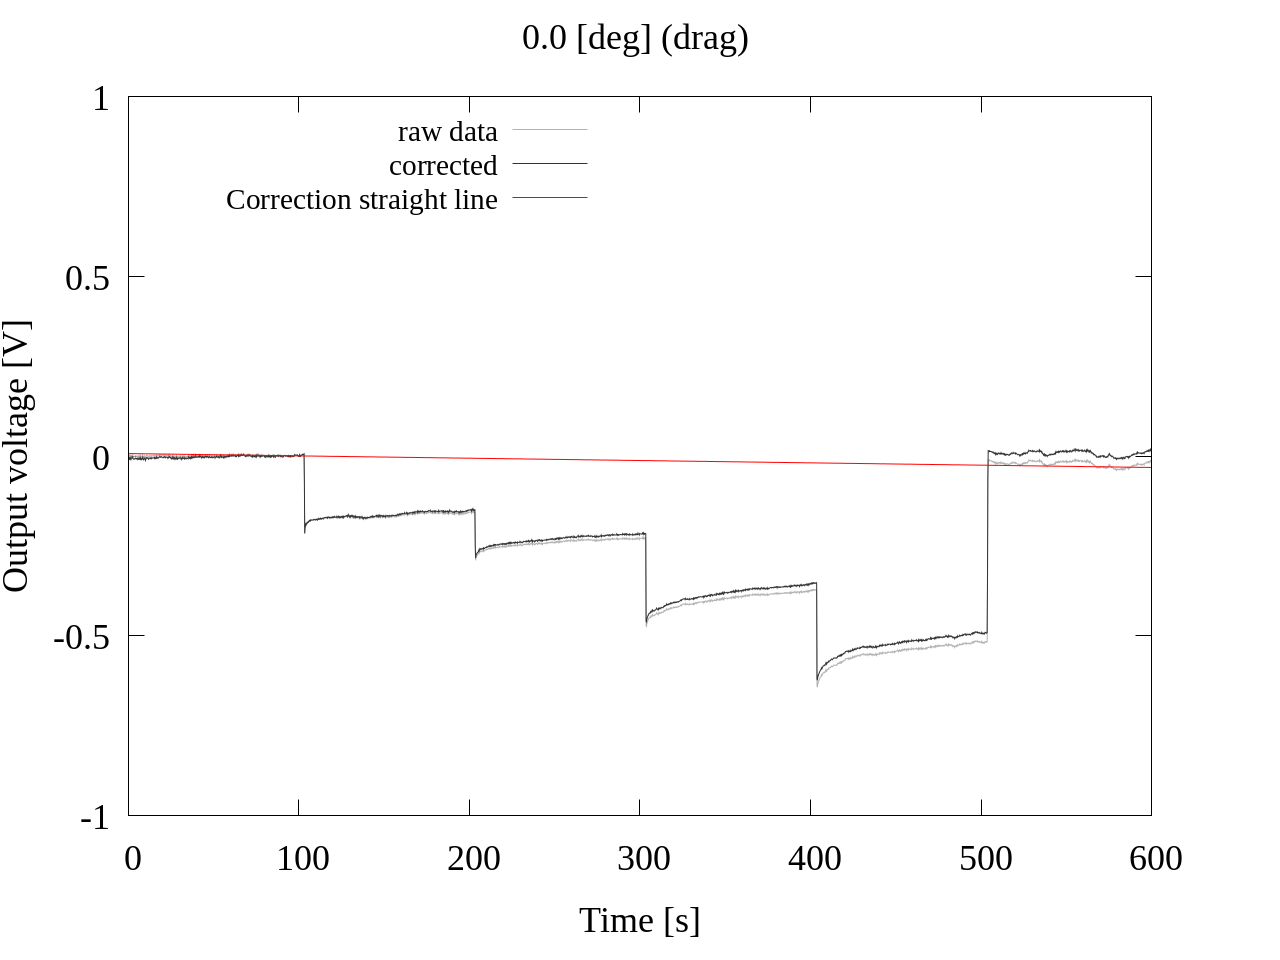
\includegraphics[width=95mm]{../../02_workspace/result/2-1/plot/02-2_drag/02_drag-drift_0.png}
		\subcaption{Drag}
		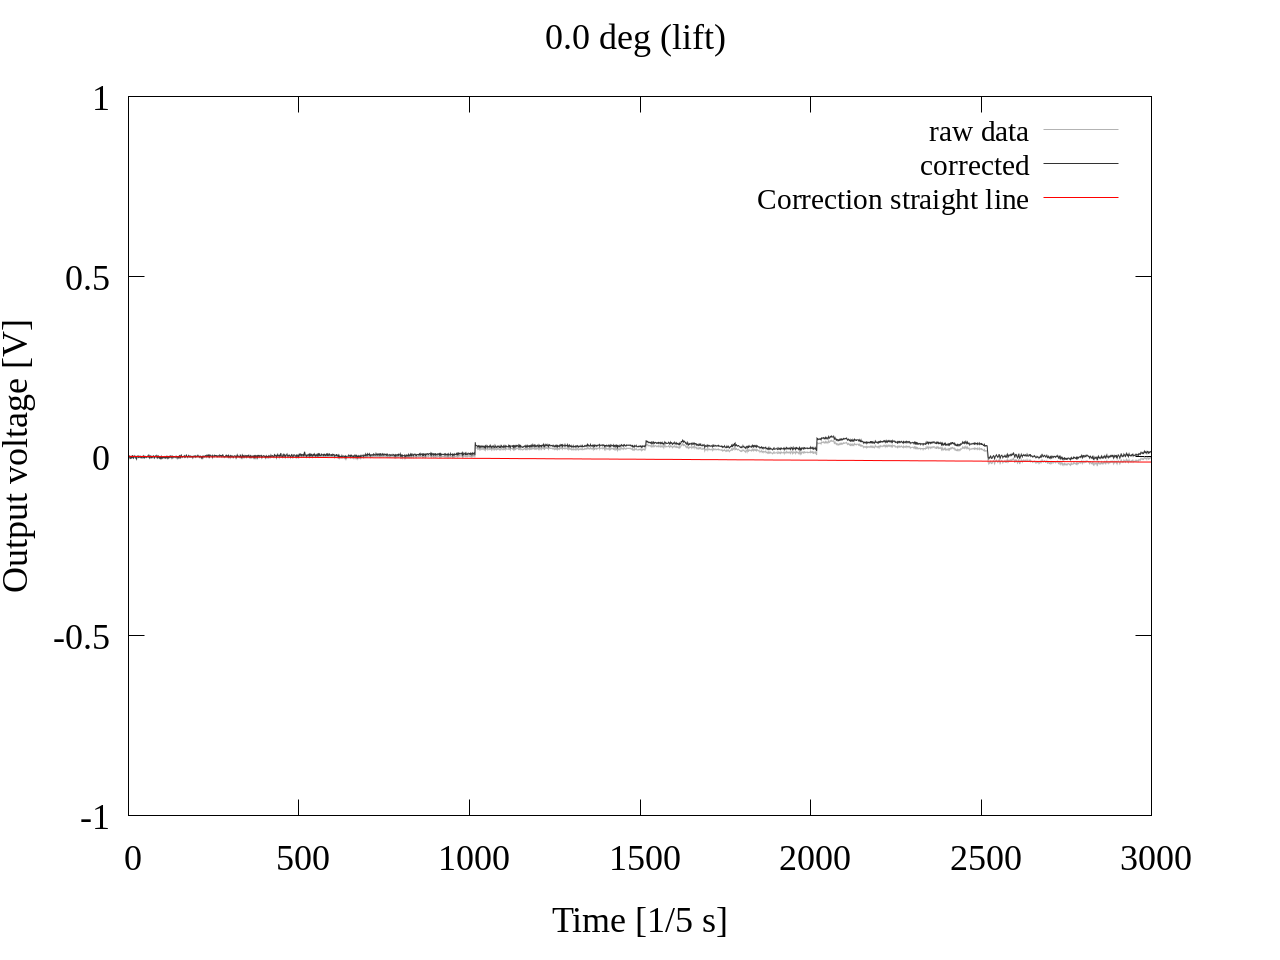
\includegraphics[width=95mm]{../../02_workspace/result/2-1/plot/02-3_lift/02_lift-drift_0.png}
		\subcaption{Lift}
    \caption{Drift corrected voltage (strain sensors) : 0 [deg]}
	\end{center}
\end{figure}

\newpage

\subsubsection{各距離における平均値の算出}

測定データの時間経過に沿って,プログラムの適用範囲を定め,
以下の手順からそれぞれのデータ範囲における出力電圧について平均値を算出した.

\begin{enumerate}[(1)]
	\item 各押込距離において測定した40秒間(計200点)のデータを使用
	\item 前後5秒(各25点)のデータを除いた30秒間(計150点)のデータの平均値を算出する
\end{enumerate}

以下のFig. にロードセルの出力電圧について平均値を算出した結果を示す.

\begin{figure}[htbp]
	\footnotesize
	\begin{center}
		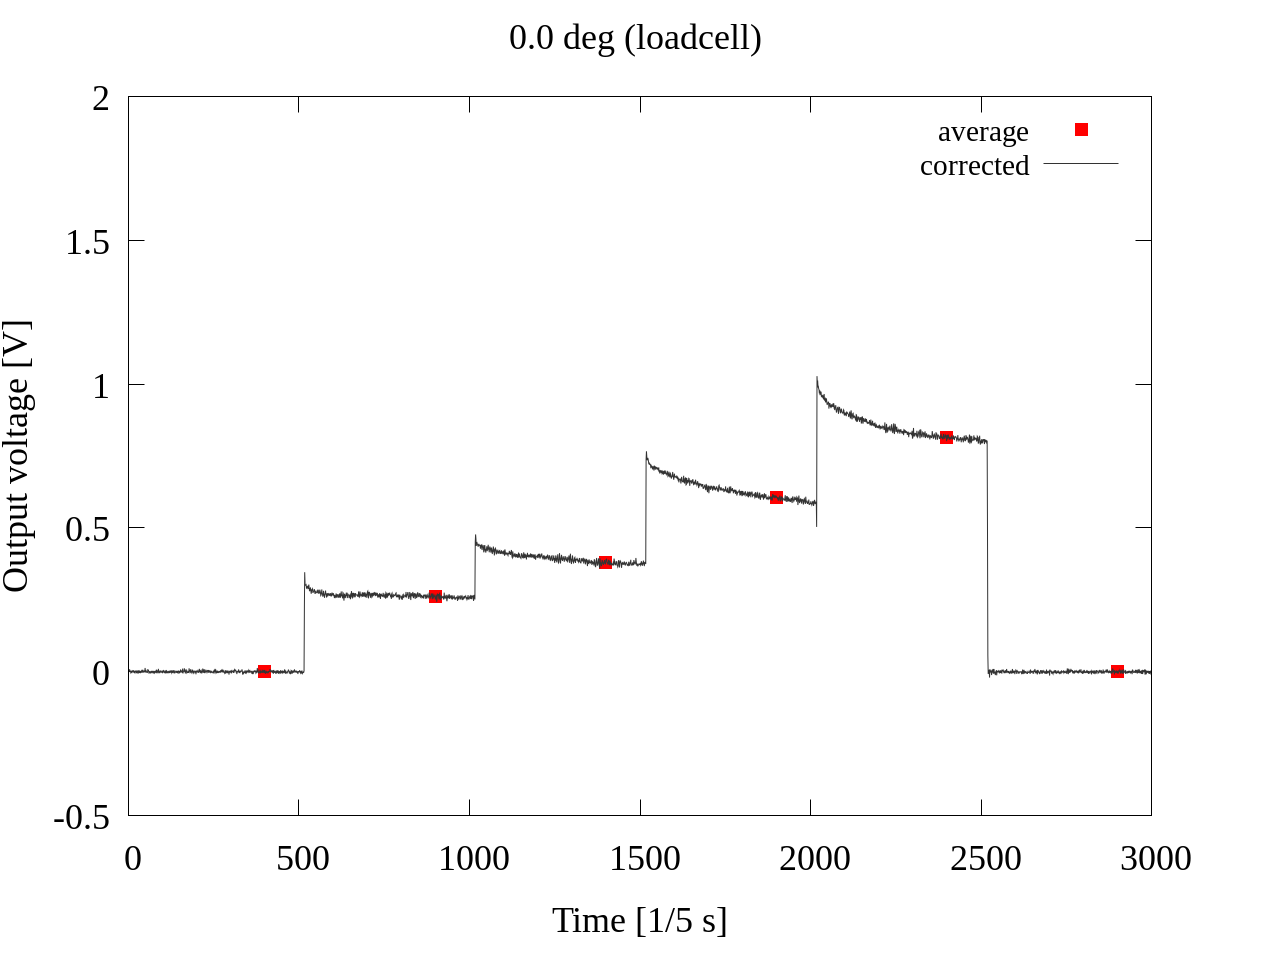
\includegraphics[width=95mm]{../../02_workspace/result/2-1/plot/03-1_loadcell/03_loadcell_average_0.png}
		\caption{Each distance average voltage (load cell) : 0 [deg]}
	\end{center}
\end{figure}

また,以下のFig.に抗力及び揚力方向のひずみセンサの出力電圧について
同様のプログラムを用いて平均値の算出を行った結果を示す.

\begin{figure}[htbp]
	\begin{minipage}[b]{0.45\linewidth}
		\centering
		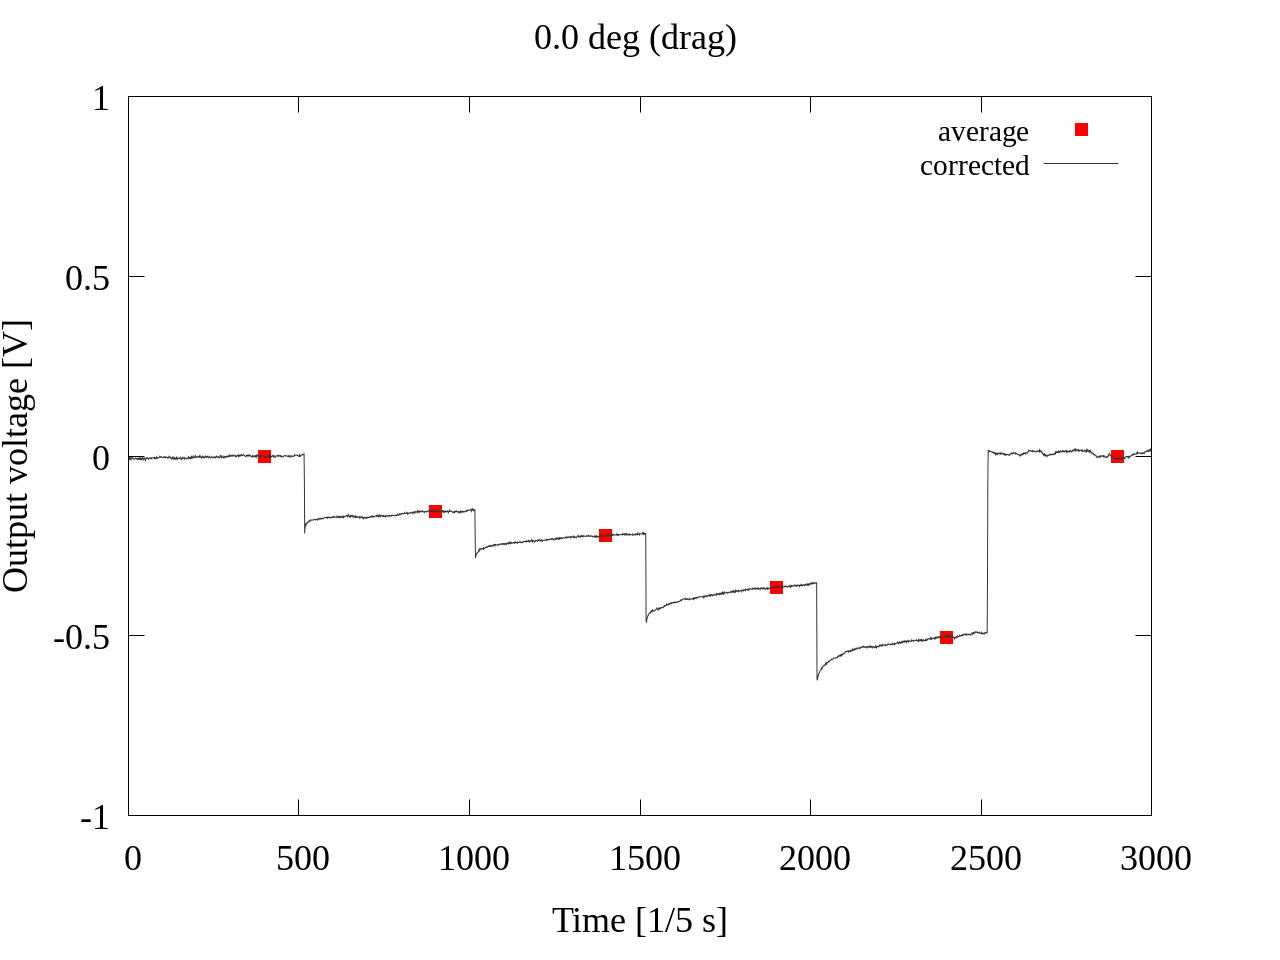
\includegraphics[width=65mm]{../../02_workspace/result/2-1/plot/03-2_drag/03_drag_average_0.png}
		\subcaption{Drag}
	\end{minipage}
	\begin{minipage}[b]{0.45\linewidth}
		\centering
		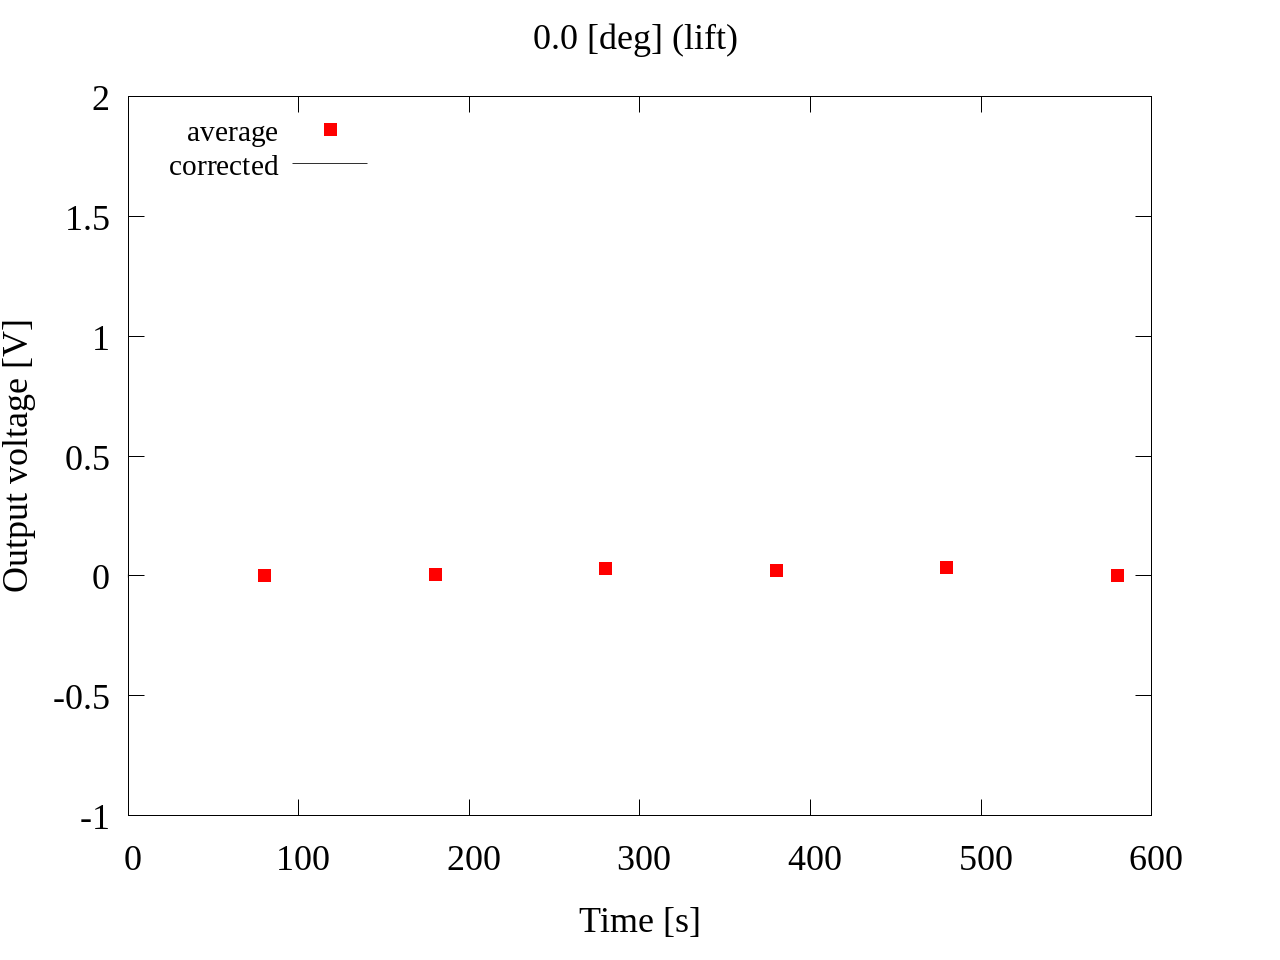
\includegraphics[width=65mm]{../../02_workspace/result/2-1/plot/03-3_lift/03_lift_average_0.png}
		\subcaption{Lift}
	\end{minipage}
  \caption{Each distance average voltage (strain sensors) : 0 [deg]}
\end{figure}

\newpage

\subsubsection{出力電圧勾配の算出}

以下のFig. に,以上の過程から算出された実験結果の出力電圧勾配を示す.\\
ここで,出力電圧勾配は,平均値を用いて最小二乗法から算出した傾きの値を採用している.
なお,以下に示す結果は1回目の測定結果における 0,30, 45,60, 90, 180 [deg]である.

\begin{figure}[htbp]
    \begin{minipage}[b]{0.45\linewidth}
      \centering
      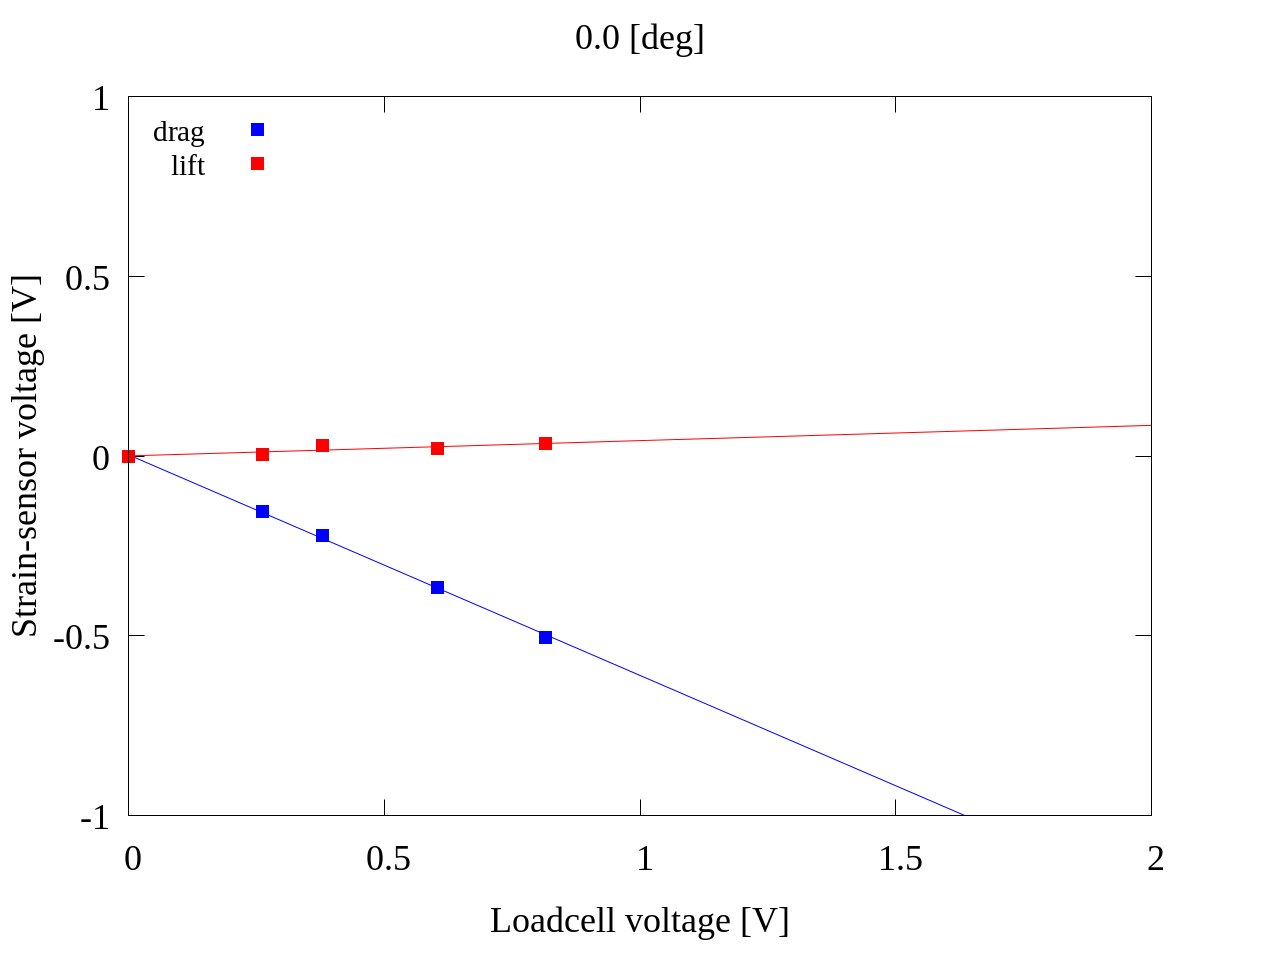
\includegraphics[width=65mm]{../../02_workspace/result/2-1/plot/04/04_linear_0.png}
      \subcaption{0 [deg]}
    \end{minipage}
    \begin{minipage}[b]{0.45\linewidth}
      \centering
      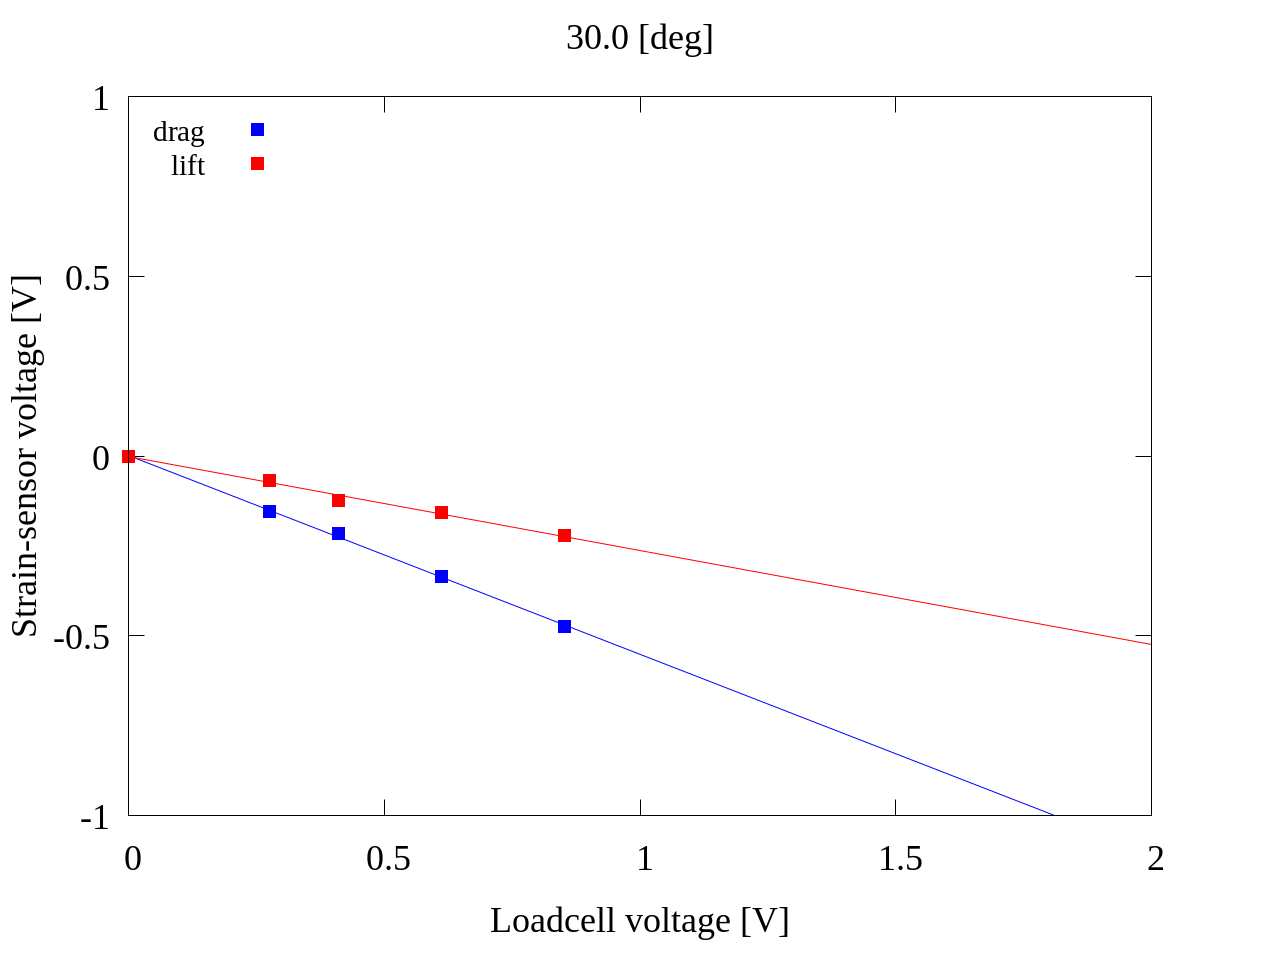
\includegraphics[width=65mm]{../../02_workspace/result/2-1/plot/04/04_linear_300.png}
      \subcaption{30 [deg]}
    \end{minipage} \\
    \begin{minipage}[b]{0.45\linewidth}
        \centering
        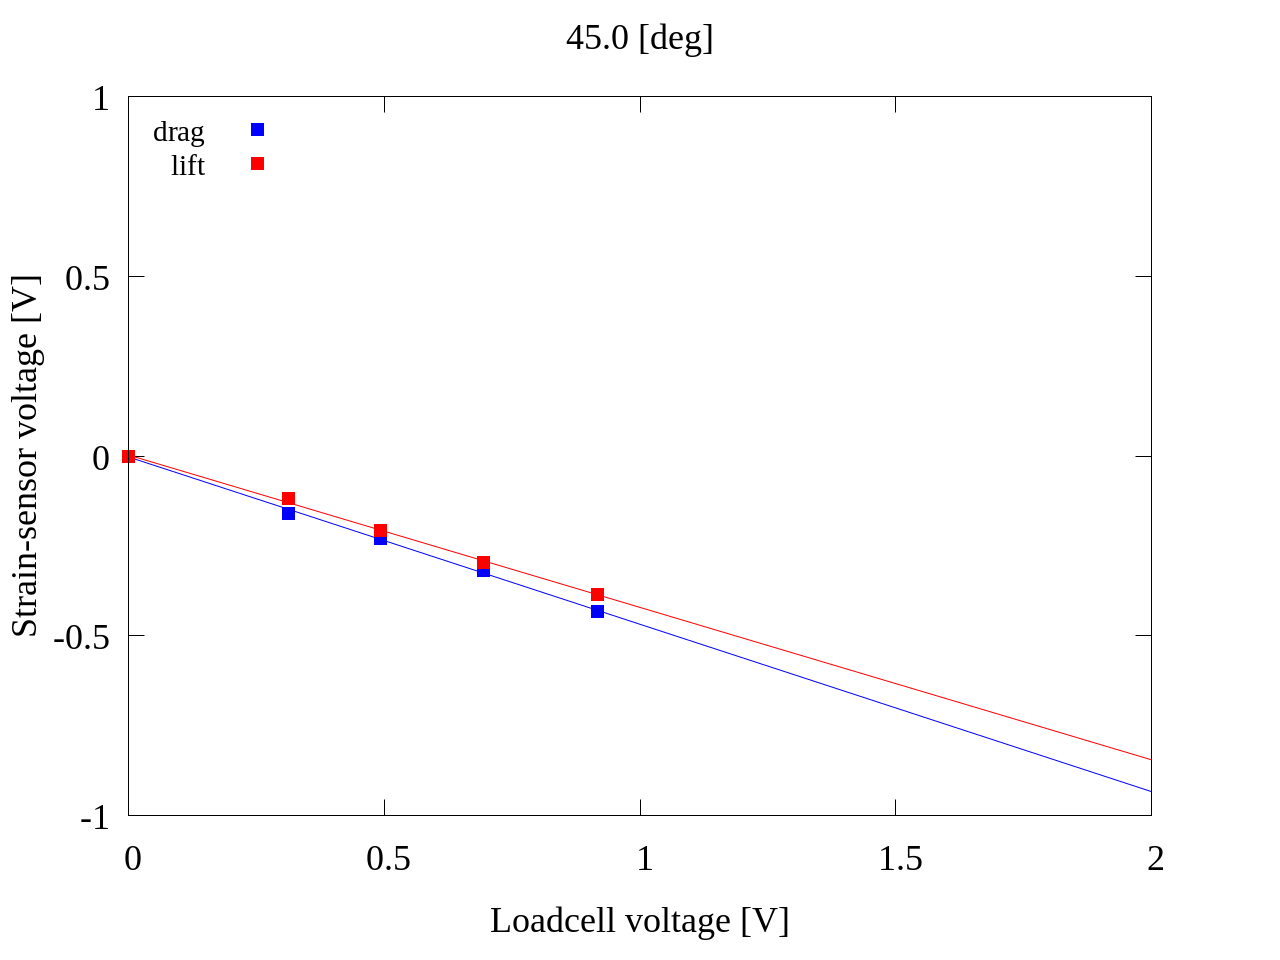
\includegraphics[width=65mm]{../../02_workspace/result/2-1/plot/04/04_linear_450.png}
        \subcaption{45 [deg]}
      \end{minipage}
      \begin{minipage}[b]{0.45\linewidth}
        \centering
        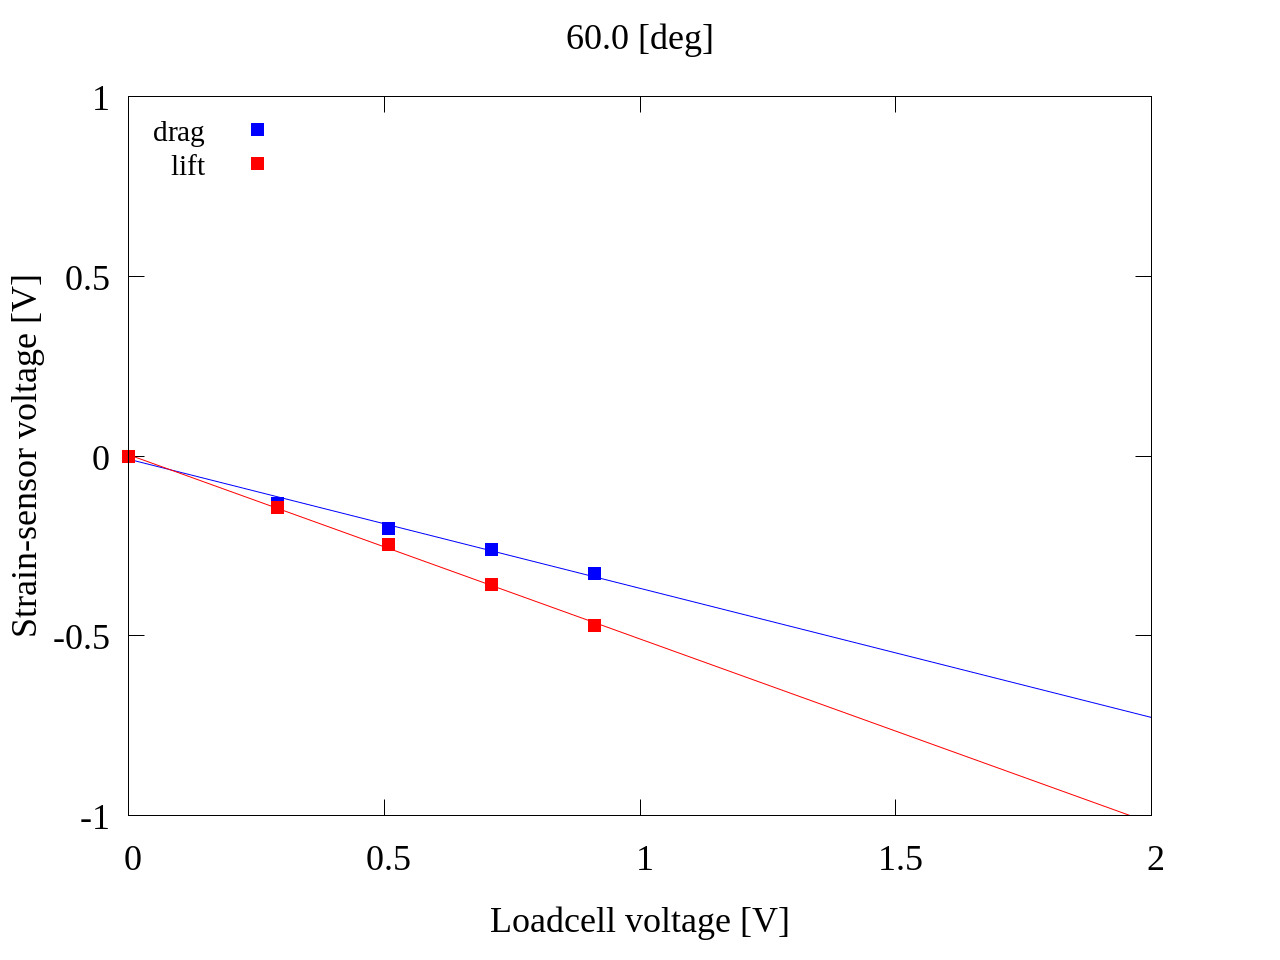
\includegraphics[width=65mm]{../../02_workspace/result/2-1/plot/04/04_linear_600.png}
        \subcaption{60 [deg]}
      \end{minipage} \\
      \begin{minipage}[b]{0.45\linewidth}
        \centering
        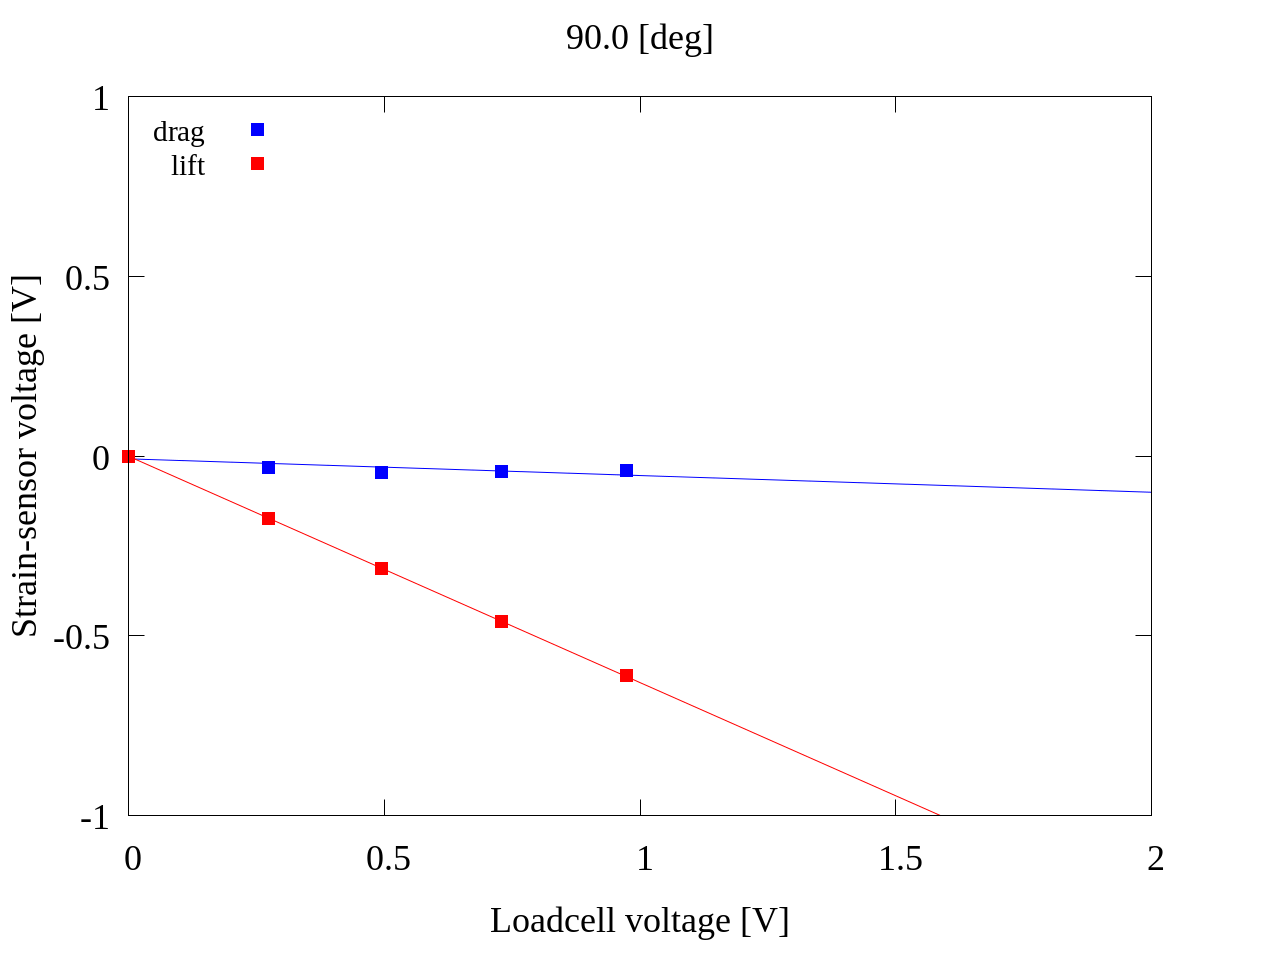
\includegraphics[width=65mm]{../../02_workspace/result/2-1/plot/04/04_linear_900.png}
        \subcaption{90 [deg]}
      \end{minipage}
      \begin{minipage}[b]{0.45\linewidth}
        \centering
        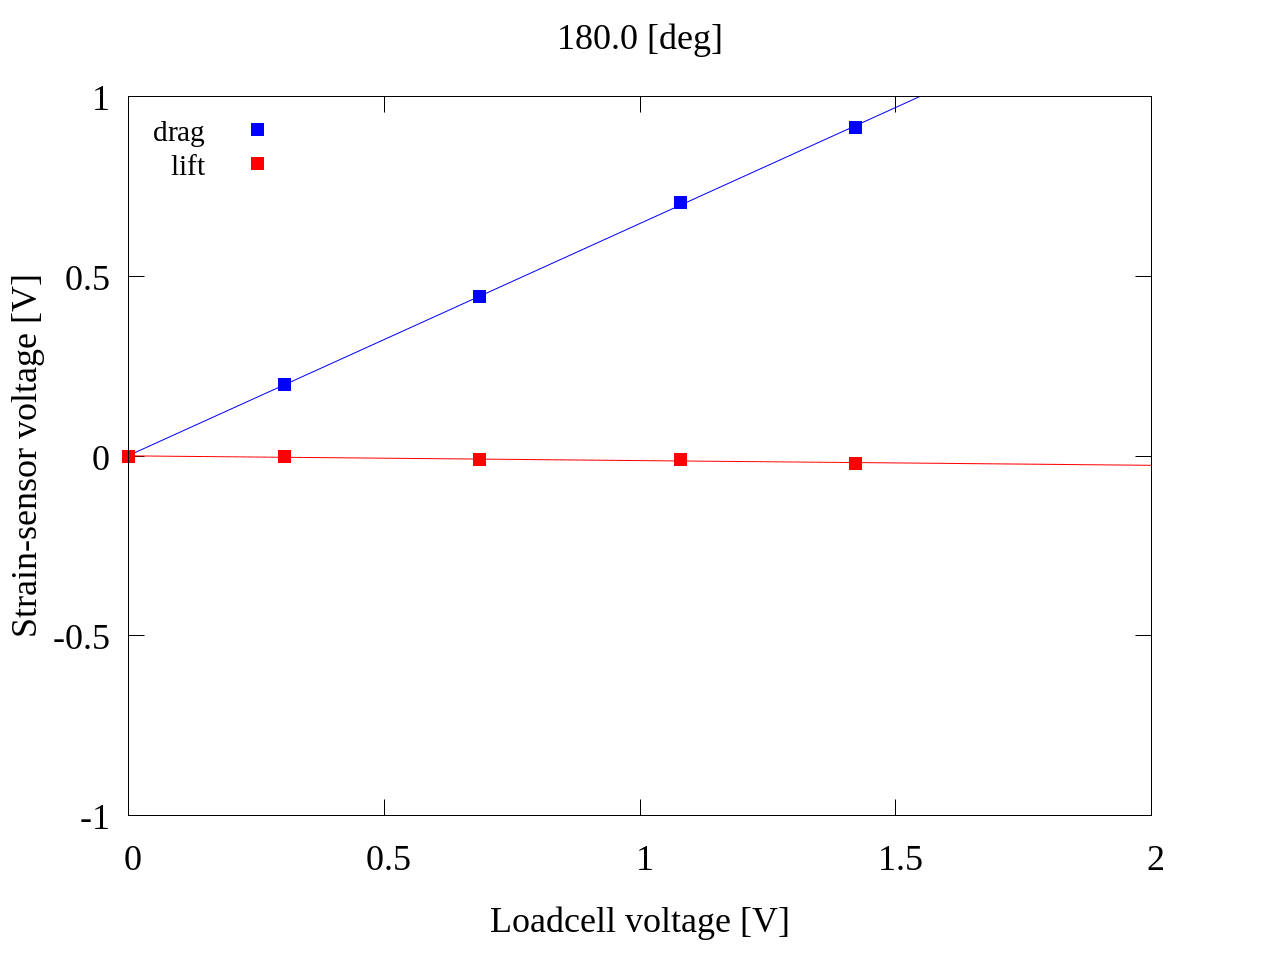
\includegraphics[width=65mm]{../../02_workspace/result/2-1/plot/04/04_linear_1800.png}
        \subcaption{180 [deg]}
      \end{minipage}
      \caption{Output voltage gradient}
    \end{figure}

% \begin{figure}[htbp]
%     \begin{minipage}[b]{0.45\linewidth}
%       \centering
%       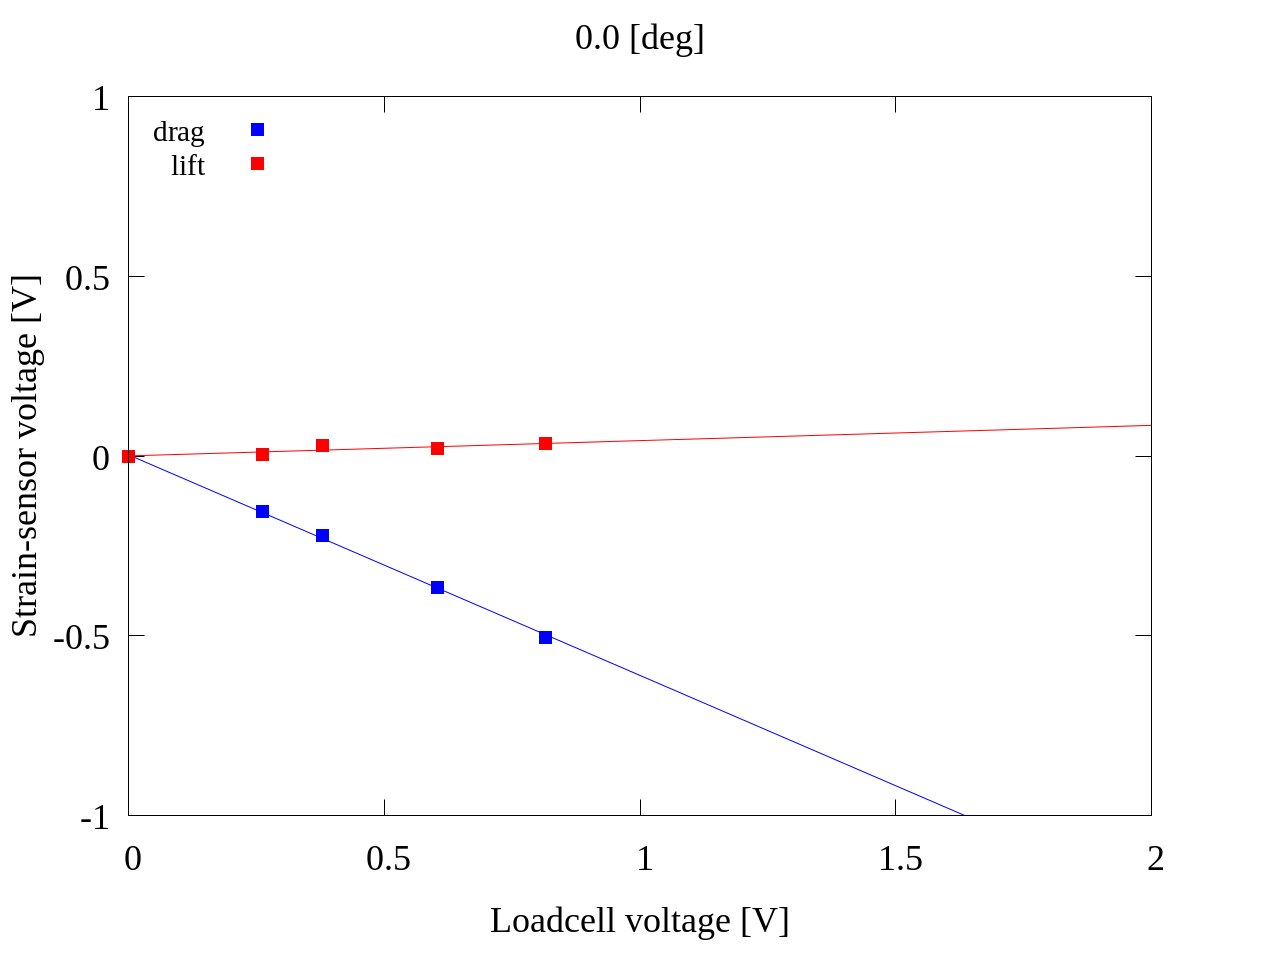
\includegraphics[width=65mm]{../../02_workspace/result/2-1/plot/04/04_linear_0.png}
%       \subcaption{0 [deg]}
%     \end{minipage}
%     \begin{minipage}[b]{0.45\linewidth}
%       \centering
%       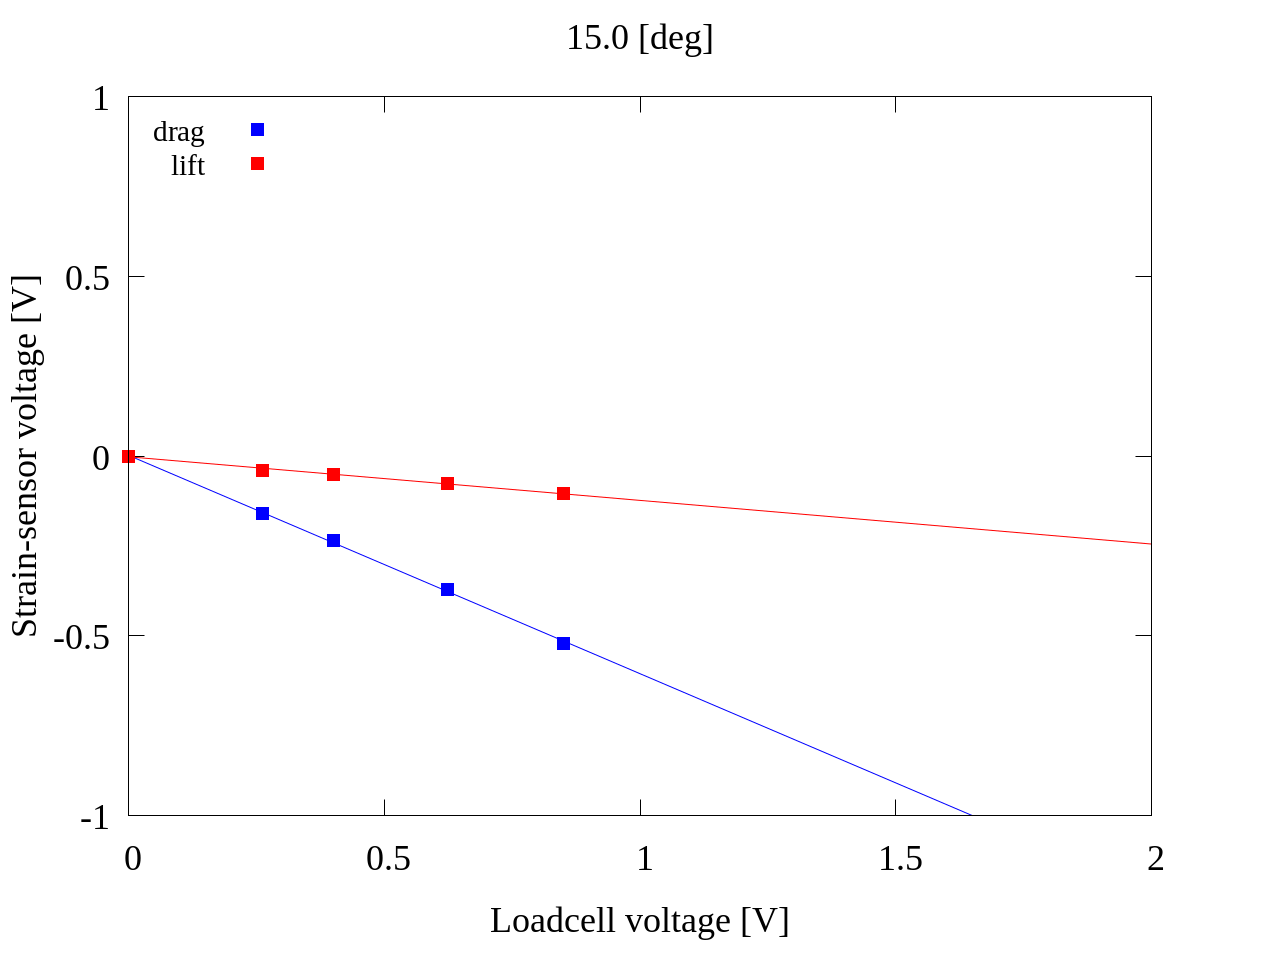
\includegraphics[width=65mm]{../../02_workspace/result/2-1/plot/04/04_linear_150.png}
%       \subcaption{15 [deg]}
%     \end{minipage} \\
%     \begin{minipage}[b]{0.45\linewidth}
%         \centering
%         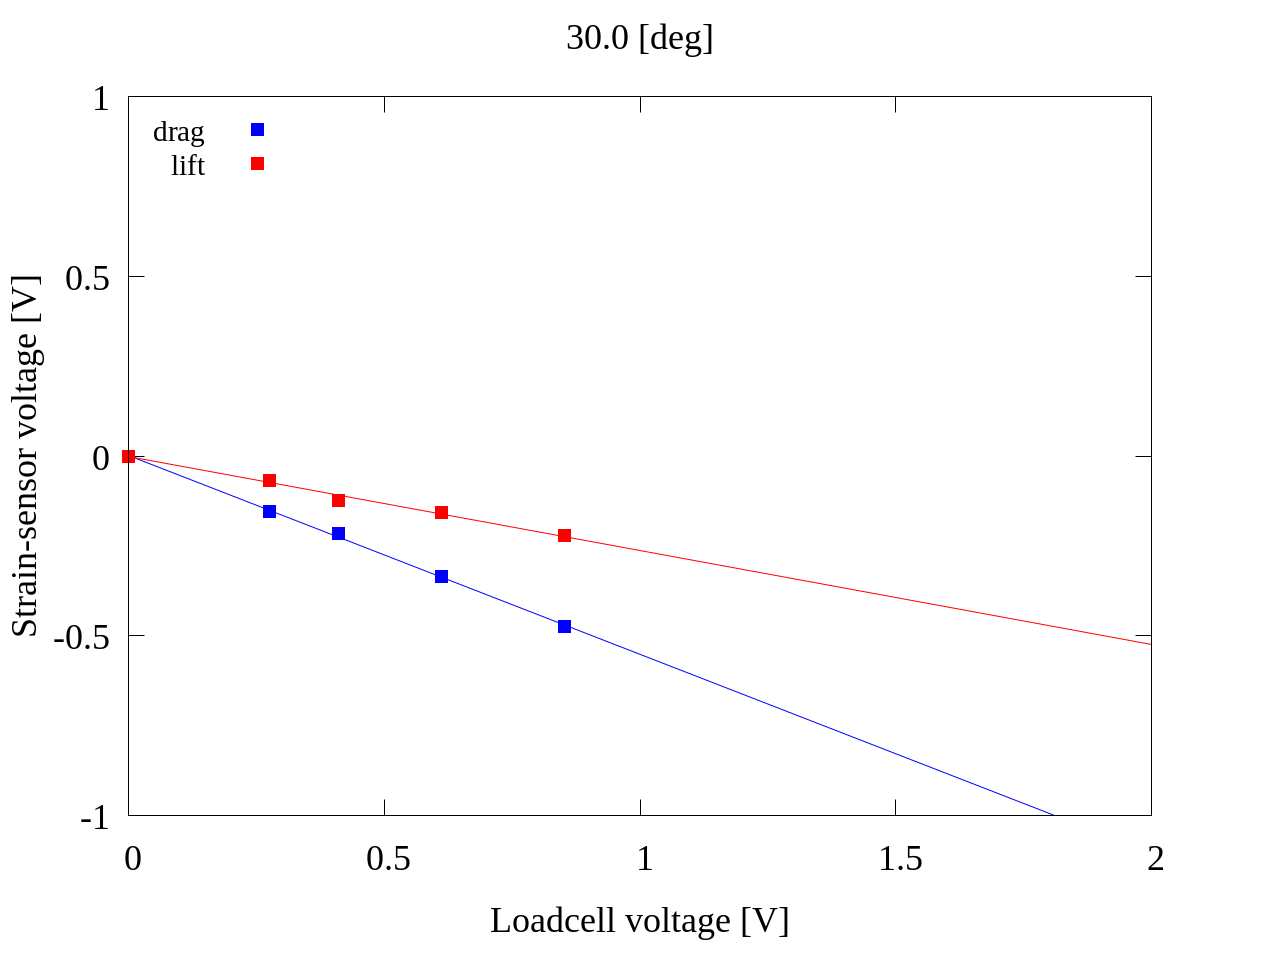
\includegraphics[width=65mm]{../../02_workspace/result/2-1/plot/04/04_linear_300.png}
%         \subcaption{30 [deg]}
%       \end{minipage}
%       \begin{minipage}[b]{0.45\linewidth}
%         \centering
%         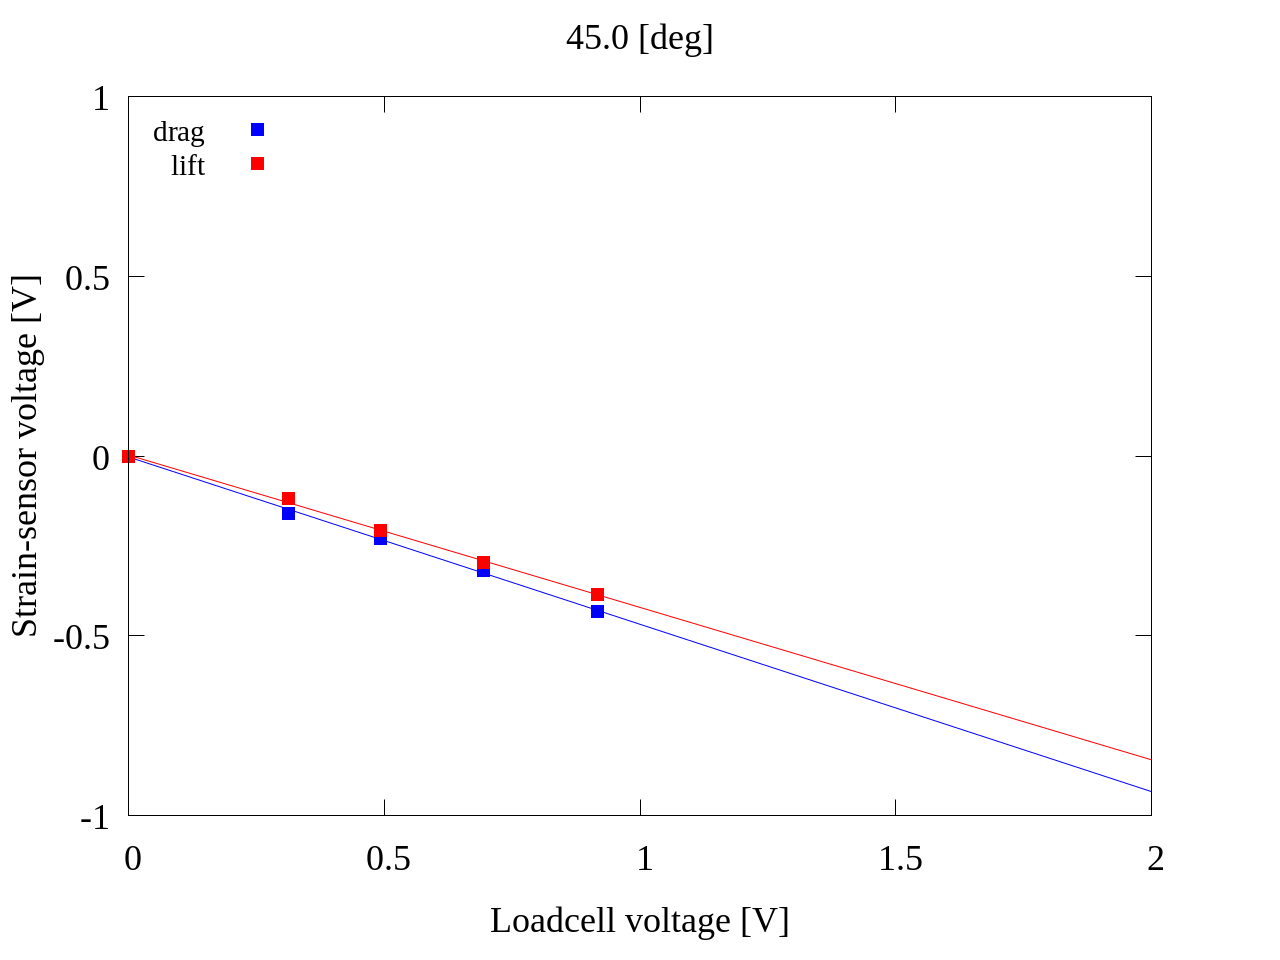
\includegraphics[width=65mm]{../../02_workspace/result/2-1/plot/04/04_linear_450.png}
%         \subcaption{45 [deg]}
%       \end{minipage} \\
%       \begin{minipage}[b]{0.45\linewidth}
%         \centering
%         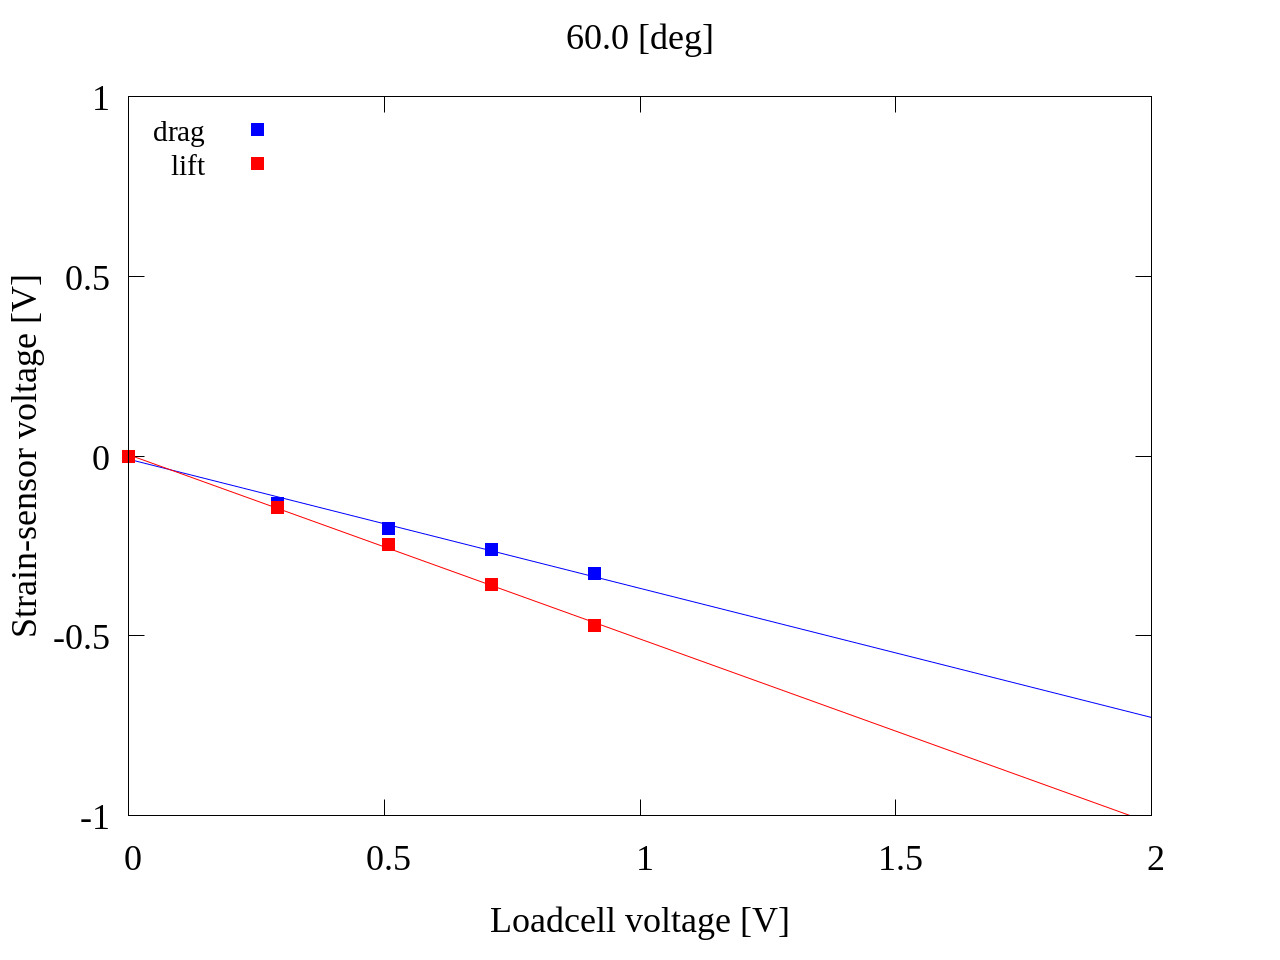
\includegraphics[width=65mm]{../../02_workspace/result/2-1/plot/04/04_linear_600.png}
%         \subcaption{60 [deg]}
%       \end{minipage}
%       \begin{minipage}[b]{0.45\linewidth}
%         \centering
%         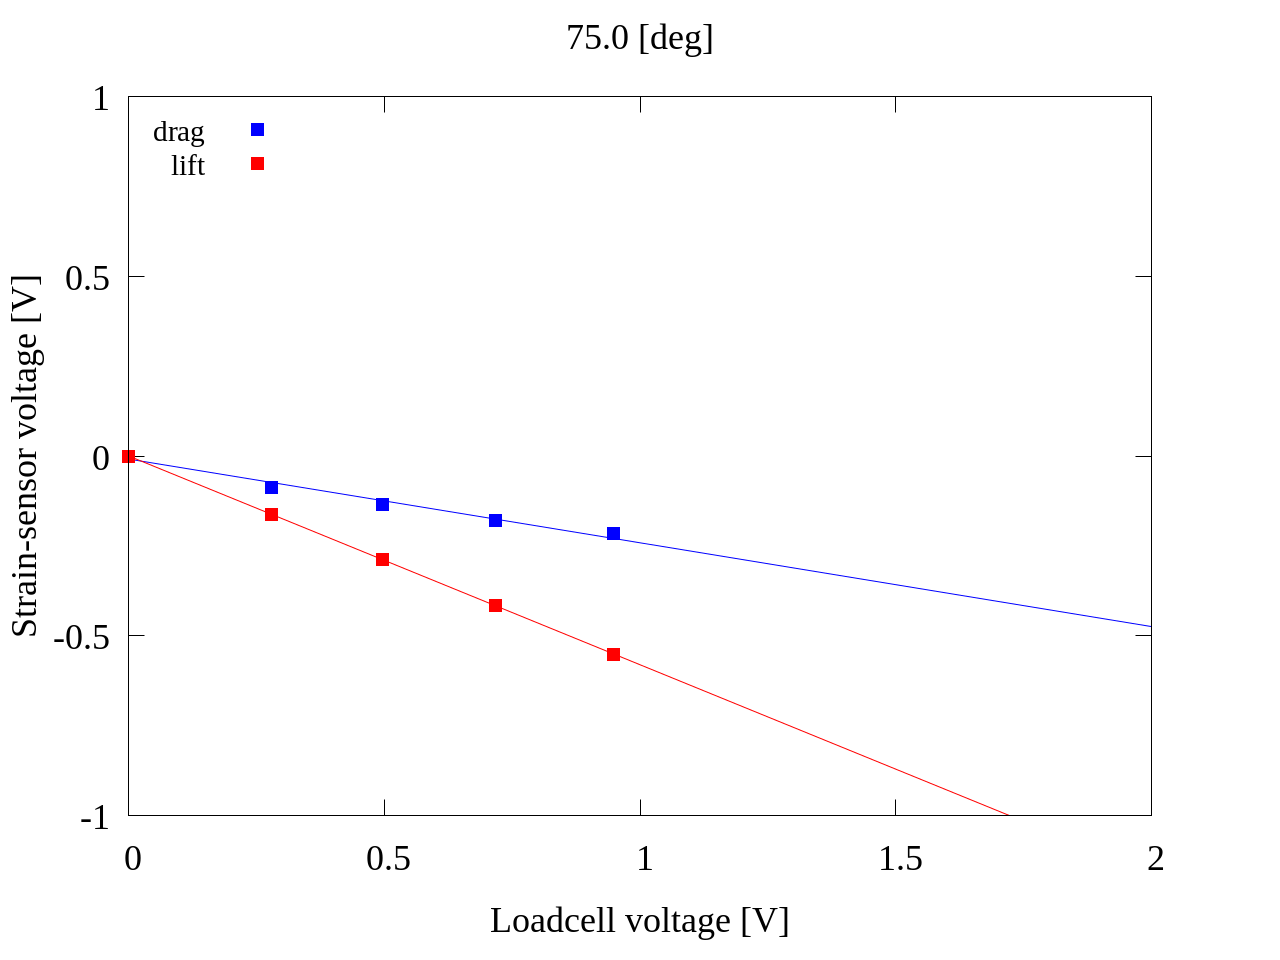
\includegraphics[width=65mm]{../../02_workspace/result/2-1/plot/04/04_linear_750.png}
%         \subcaption{75 [deg]}
%       \end{minipage}
%     \end{figure}

%     \begin{figure}
%       \begin{minipage}[b]{0.45\linewidth}
%         \centering
%       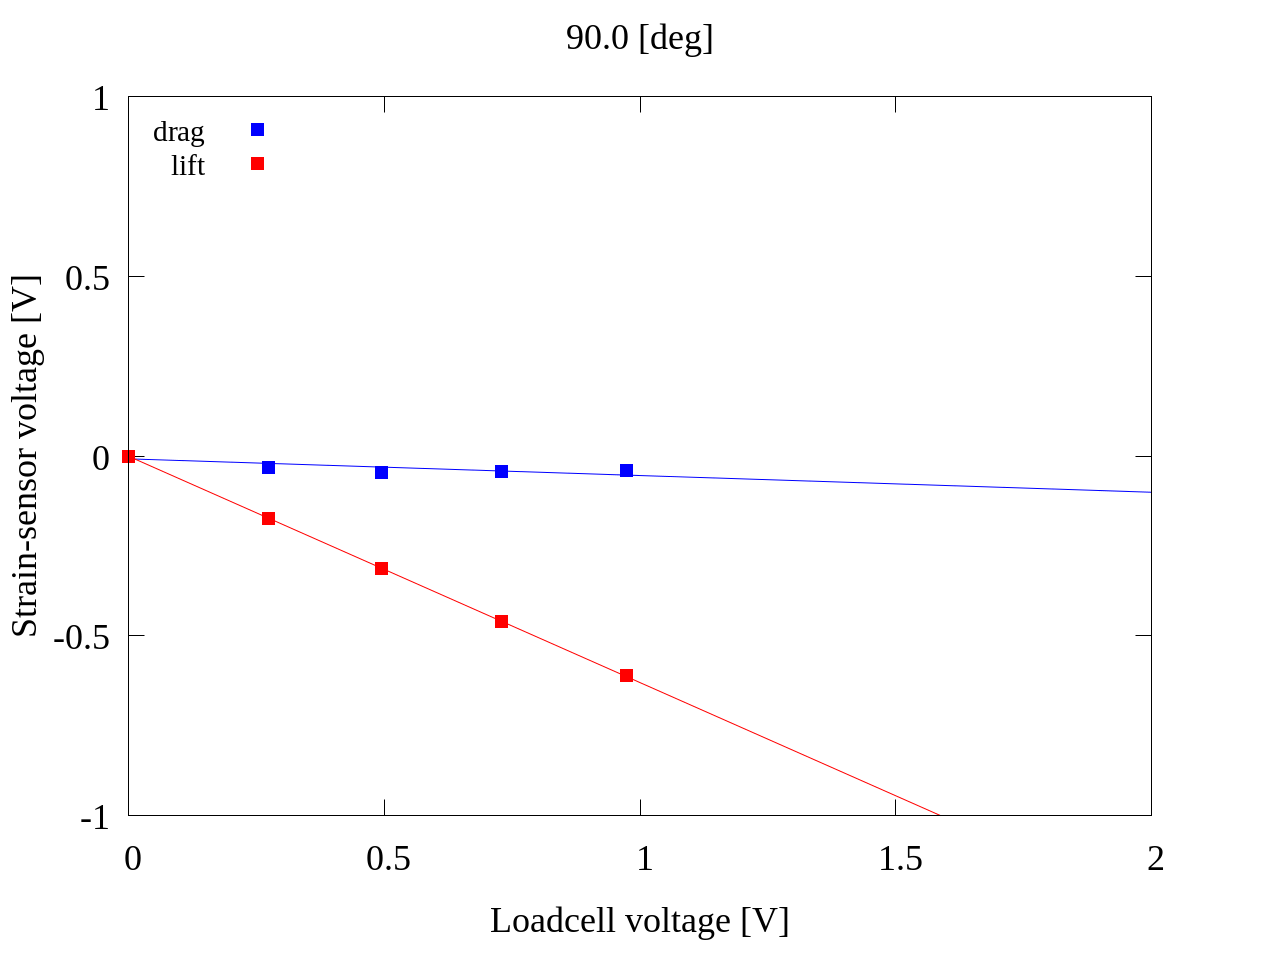
\includegraphics[width=65mm]{../../02_workspace/result/2-1/plot/04/04_linear_900.png}
%       \subcaption{90 [deg]}
%     \end{minipage}
%     \begin{minipage}[b]{0.45\linewidth}
%         \centering
%         \includegraphics[width=65mm]{../../02_workspace/result/2-1/plot/04/04_linear_1050.png}
%         \subcaption{105 [deg]}
%       \end{minipage}\\
%       \begin{minipage}[b]{0.45\linewidth}
%         \centering
%         \includegraphics[width=65mm]{../../02_workspace/result/2-1/plot/04/04_linear_1200.png}
%         \subcaption{120 [deg]}
%       \end{minipage}
%       \begin{minipage}[b]{0.45\linewidth}
%         \centering
%         \includegraphics[width=65mm]{../../02_workspace/result/2-1/plot/04/04_linear_1350.png}
%         \subcaption{135 [deg]}
%       \end{minipage}\\
%       \begin{minipage}[b]{0.45\linewidth}
%         \centering
%         \includegraphics[width=65mm]{../../02_workspace/result/2-1/plot/04/04_linear_1500.png}
%         \subcaption{150 [deg]}
%       \end{minipage} 
%       \begin{minipage}[b]{0.45\linewidth}
%         \centering
%         \includegraphics[width=65mm]{../../02_workspace/result/2-1/plot/04/04_linear_1650.png}
%         \subcaption{165 [deg]}
%       \end{minipage}
%     \end{figure}

%     \begin{figure}
%       \begin{minipage}[b]{0.45\linewidth}
%         \centering
%         \includegraphics[width=65mm]{../../02_workspace/result/2-1/plot/04/04_linear_1800.png}
%         \subcaption{180 [deg]}
%       \end{minipage}
%       \begin{minipage}[b]{0.45\linewidth}
%         \centering
%         \includegraphics[width=65mm]{../../02_workspace/result/2-1/plot/04/04_linear_1950.png}
%         \subcaption{195 [deg]}
%       \end{minipage}\\
%       \begin{minipage}[b]{0.45\linewidth}
%         \centering
%         \includegraphics[width=65mm]{../../02_workspace/result/2-1/plot/04/04_linear_2100.png}
%         \subcaption{210 [deg]}
%       \end{minipage}
%       \begin{minipage}[b]{0.45\linewidth}
%         \centering
%         \includegraphics[width=65mm]{../../02_workspace/result/2-1/plot/04/04_linear_2250.png}
%         \subcaption{225 [deg]}
%       \end{minipage}\\
%       \begin{minipage}[b]{0.45\linewidth}
%         \centering
%         \includegraphics[width=65mm]{../../02_workspace/result/2-1/plot/04/04_linear_2400.png}
%         \subcaption{240 [deg]}
%       \end{minipage}
%       \begin{minipage}[b]{0.45\linewidth}
%         \centering
%         \includegraphics[width=65mm]{../../02_workspace/result/2-1/plot/04/04_linear_2550.png}
%         \subcaption{255 [deg]}
%       \end{minipage}
%     \end{figure}

%     \begin{figure}
%       \begin{minipage}[b]{0.45\linewidth}
%         \centering
%         \includegraphics[width=65mm]{../../02_workspace/result/2-1/plot/04/04_linear_2700.png}
%         \subcaption{270 [deg]}
%       \end{minipage}
%       \begin{minipage}[b]{0.45\linewidth}
%         \centering
%         \includegraphics[width=65mm]{../../02_workspace/result/2-1/plot/04/04_linear_2850.png}
%         \subcaption{285 [deg]}
%       \end{minipage}\\
%       \begin{minipage}[b]{0.45\linewidth}
%         \centering
%         \includegraphics[width=65mm]{../../02_workspace/result/2-1/plot/04/04_linear_3000.png}
%         \subcaption{300 [deg]}
%       \end{minipage}
%       \begin{minipage}[b]{0.45\linewidth}
%         \centering
%         \includegraphics[width=65mm]{../../02_workspace/result/2-1/plot/04/04_linear_3150.png}
%         \subcaption{315 [deg]}
%       \end{minipage}\\
%       \begin{minipage}[b]{0.45\linewidth}
%         \centering
%         \includegraphics[width=65mm]{../../02_workspace/result/2-1/plot/04/04_linear_3300.png}
%         \subcaption{330 [deg]}
%       \end{minipage}
%       \begin{minipage}[b]{0.45\linewidth}
%         \centering
%         \includegraphics[width=65mm]{../../02_workspace/result/2-1/plot/04/04_linear_3450.png}
%         \subcaption{345 [deg]}
%       \end{minipage}
% \end{figure}

\newpage

また,出力電圧勾配について各角度における算出値をプロットしたものを以下のFig.,Fig.に示す.
なお,ここで示す出力電圧勾配の値は5回実施した実験結果の平均値である.

\begin{figure}[htbp]
		\centering
		\includegraphics[width=95mm]{../../02_workspace/result/2-ex/plot/21/21-1_summary_drag.png}
		\subcaption{Drag}
		\includegraphics[width=95mm]{../../02_workspace/result/2-ex/plot/21/21-1_summary_lift.png}
		\subcaption{Lift}
    \caption{5 times average of voltage gradient}
\end{figure}

\newpage

\subsection{校正理論の適用とその結果}
実験結果について作成した補正理論を適用し,水槽座標系における出力電圧勾配への変換を行う.

\subsubsection{補正理論[2]の適用}
Fig.,Fig.について,座標系のオフセットにおける補正理論である
式()の適用後の出力電圧勾配$v_{x'1}$,$v_{y'1}$を以下のFig.,Fig.に示す.
なお,補正の際に用いたオフセット距離$\Delta x$,$\Delta y$は
実験の際に測定した以下のTable の数値を用いて行った.

\begin{figure}[htbp]
		\centering
		\includegraphics[width=95mm]{../../02_workspace/result/2-ex/plot/21/21-2_corrected_offset_drag.png}
		\subcaption{Drag}
		\includegraphics[width=95mm]{../../02_workspace/result/2-ex/plot/21/21-2_corrected_offset_lift.png}
		\subcaption{Lift}
    \caption{Offset corrected voltage gradient}
\end{figure}

\begin{table}[htbp]
  \scalefont{0.9}
  \begin{center}
      \caption{Offset length}
      \begin{tabular}{|p{30mm}|p{20mm}|p{20mm}|}
          \hline
          \multicolumn{1}{|c|}{$\Delta x$ [mm]} & \multicolumn{1}{|c|}{$\Delta y$ [mm]} \\ \hline
          \multicolumn{1}{|c|}{0.09}           & \multicolumn{1}{|c|}{0.06}           \\ \hline
      \end{tabular}
  \end{center}
\end{table}

\newpage

\subsubsection{補正理論[3]の適用}
Fig.,Fig.について,式()のラグランジュ補間公式によって
二次補間の適用後の出力電圧勾配$v_{x'2}$,$v_{y'2}$を以下のFig.,Fig.に示す.

\begin{figure}[htbp]
		\centering
		\includegraphics[width=95mm]{../../02_workspace/result/2-ex/plot/21/21-3_interpolated_drag.png}
		\caption{Interpolated : drag (Average)}
		\includegraphics[width=95mm]{../../02_workspace/result/2-ex/plot/21/21-3_interpolated_lift.png}
		\caption{Interpolated : lift (Average)}
\end{figure}

\newpage

\subsubsection{補正理論[1]の適用}
はじめに,水槽座標系からの回転角$\theta_x$,$\theta_y$を推定するため,
Fig.,Fig.の結果に離散フーリエ変換を適用し,波数1の成分から$\theta_x$,$\theta_y$を算出する.
ここで,その結果を以下のFig.,Fig.に示す.

\begin{figure}
        \begin{minipage}[b]{0.45\linewidth}
        \centering
        \includegraphics[width=65mm]{../../02_workspace/result/2-ex/plot/07/07-3_dft-drag.png}
        \subcaption{Drag}
      \end{minipage}
      \begin{minipage}[b]{0.45\linewidth}
        \centering
        \includegraphics[width=65mm]{../../02_workspace/result/2-ex/plot/07/07-4_dft-lift.png}
        \subcaption{Lift}
      \end{minipage}
      \caption{DFT spectrum}
\end{figure}

Fig.,Fig.をみると,どちらもピークは波数1のときにあり,
波の特徴を正しく捉えられていることがわかる.
また,このとき算出された波数1の値について,以下のTable に示す.

\begin{table}[htbp]
  \begin{center}
      \caption{DFT result value : wave 1}
      \begin{tabular}{|p{30mm}|p{20mm}|p{20mm}|}
          \hline
          \multicolumn{1}{|c|}{}     & \multicolumn{1}{|c|}{Re}    & \multicolumn{1}{|c|}{Im}   \\ \hline
          \multicolumn{1}{|c|}{Drag} & \multicolumn{1}{|c|}{-7.503} & \multicolumn{1}{|c|}{1.022}  \\ \hline
          \multicolumn{1}{|c|}{Lift} & \multicolumn{1}{|c|}{0.664}  & \multicolumn{1}{|c|}{7.559} \\ \hline
      \end{tabular}
  \end{center}
\end{table}

ここで,式(),式()を用いてそれぞれの回転角$\theta_x$,$\theta_y$を算出する.
余弦波からの位相角をそれぞれ$\phi_x$,$\phi_y$とすると,以下のように算出される.
\begin{align}
	\phi_x &= \arctan \left(\frac{1.022}{-7.503}\right) \cdot \frac{180}{\pi} = 172.243\; [\mathrm{deg}]\\
  \notag \\
	\phi_y &= \arctan \left(\frac{7.559}{0.664}\right) \cdot \frac{180}{\pi} = 84.979\; [\mathrm{deg}]
\end{align}

したがって,回転角$\theta_x$,$\theta_y$は,以下のように表される.
\begin{align}
	\theta_x &= 180 - \phi_x = 7.757 \; [\mathrm{deg}]\\
	\theta_y &= 90 - \phi_y = 5.019 \; [\mathrm{deg}]
\end{align}

また,その算出結果を以下のTable に示す.

\begin{table}[htbp]
  \begin{center}
      \caption{Specified rotation angle}
      \begin{tabular}{|p{30mm}|p{20mm}|p{20mm}|}
          \hline
          \multicolumn{1}{|c|}{$\theta_x$ [deg]} & \multicolumn{1}{|c|}{$\theta_y$ [deg]} \\ \hline
          \multicolumn{1}{|c|}{7.757}           & \multicolumn{1}{|c|}{5.019}           \\ \hline
      \end{tabular}
  \end{center}
\end{table}

\newpage
推定した回転角$\theta_x$,$\theta_y$を用いて
Fig.,Fig.について,座標系の回転における補正理論である
式()の適用後の出力電圧勾配$v_x$,$v_y$を以下のFig.,Fig.に示す.

\begin{figure}[htbp]
		\centering
		\includegraphics[width=95mm]{../../02_workspace/result/2-ex/plot/21/21-4_corrected_angle_drag.png}
		\caption{Rotation corrected : drag (Average)}
		\includegraphics[width=95mm]{../../02_workspace/result/2-ex/plot/21/21-4_corrected_angle_lift.png}
		\caption{Rotation corrected : lift (Average)}
\end{figure}

\newpage

\subsubsection{実験結果における正味出力電圧}
Fig.,Fig.の値を用いて,式()から算出される正味出力電圧勾配$v_{\mathrm{net}}$の値について
以下のFig.に示す.

\begin{figure}[htbp]
  \centering
  \includegraphics[width=95mm]{../../02_workspace/result/2-ex/plot/09/09_summary-outputvoltage-net.png}
  \caption{Interpolated : drag (Average)}
\end{figure}

Fig.をみると正味出力電圧勾配$v_{net}$は周期的な変動を示していることがわかる.

\newpage

また,以下のTable に補正前の出力電圧勾配$v_d$,$v_l$と補正後の$v_x$,$v_y$,
算出された正味出力電圧勾配$v_{\mathrm{net}}$の値について示す.

\begin{table}[htbp]
    \begin{center}
        \caption{Result summary}
        \begin{tabular}{|p{20mm}|p{20mm}|p{20mm}|p{20mm}|p{20mm}|p{20mm}|}
            \hline
            \multicolumn{1}{|c|}{\textgt{$\theta$ [deg]}} & \multicolumn{1}{|c|}{\textgt{$v_d$ [V/V]}} & \multicolumn{1}{|c|}{\textgt{$v_l$ [V/V]}} & \multicolumn{1}{|c|}{\textgt{$v_x$ [V/V]}} & \multicolumn{1}{|c|}{\textgt{$v_y$ [V/V]}} & \multicolumn{1}{|c|}{\textgt{$v_{net}$ [V/V]}}\\ \hline
            \multicolumn{1}{|c|}{0}                       & \multicolumn{1}{|r|}{-0.627}                        & \multicolumn{1}{|r|}{0.063}                   & \multicolumn{1}{|r|}{-0.634}                    & \multicolumn{1}{|r|}{0.005}                   & \multicolumn{1}{|r|}{0.634}                         \\ \hline
            \multicolumn{1}{|c|}{15}                      & \multicolumn{1}{|r|}{-0.617}                        & \multicolumn{1}{|r|}{-0.103}                  & \multicolumn{1}{|r|}{-0.601}                    & \multicolumn{1}{|r|}{-0.157}                  & \multicolumn{1}{|r|}{0.621}                         \\ \hline
            \multicolumn{1}{|c|}{30}                      & \multicolumn{1}{|r|}{-0.566}                        & \multicolumn{1}{|r|}{-0.261}                  & \multicolumn{1}{|r|}{-0.528}                    & \multicolumn{1}{|r|}{-0.310}                  & \multicolumn{1}{|r|}{0.612}                         \\ \hline
            \multicolumn{1}{|c|}{45}                      & \multicolumn{1}{|r|}{-0.479}                        & \multicolumn{1}{|r|}{-0.405}                  & \multicolumn{1}{|r|}{-0.423}                    & \multicolumn{1}{|r|}{-0.444}                  & \multicolumn{1}{|r|}{0.613}                         \\ \hline
            \multicolumn{1}{|c|}{60}                      & \multicolumn{1}{|r|}{-0.365}                        & \multicolumn{1}{|r|}{-0.508}                  & \multicolumn{1}{|r|}{-0.296}                    & \multicolumn{1}{|r|}{-0.536}                  & \multicolumn{1}{|r|}{0.612}                         \\ \hline
            \multicolumn{1}{|c|}{75}                      & \multicolumn{1}{|r|}{-0.226}                        & \multicolumn{1}{|r|}{-0.582}                  & \multicolumn{1}{|r|}{-0.148}                    & \multicolumn{1}{|r|}{-0.597}                  & \multicolumn{1}{|r|}{0.615}                         \\ \hline
            \multicolumn{1}{|c|}{90}                      & \multicolumn{1}{|r|}{-0.038}                        & \multicolumn{1}{|r|}{-0.624}                  & \multicolumn{1}{|r|}{0.044}                     & \multicolumn{1}{|r|}{-0.623}                  & \multicolumn{1}{|r|}{0.624}                         \\ \hline
            \multicolumn{1}{|c|}{105}                     & \multicolumn{1}{|r|}{0.131}                         & \multicolumn{1}{|r|}{-0.618}                  & \multicolumn{1}{|r|}{0.212}                     & \multicolumn{1}{|r|}{-0.602}                  & \multicolumn{1}{|r|}{0.639}                         \\ \hline
            \multicolumn{1}{|c|}{120}                     & \multicolumn{1}{|r|}{0.296}                         & \multicolumn{1}{|r|}{-0.560}                  & \multicolumn{1}{|r|}{0.369}                     & \multicolumn{1}{|r|}{-0.531}                  & \multicolumn{1}{|r|}{0.647}                         \\ \hline
            \multicolumn{1}{|c|}{135}                     & \multicolumn{1}{|r|}{0.425}                         & \multicolumn{1}{|r|}{-0.474}                  & \multicolumn{1}{|r|}{0.486}                     & \multicolumn{1}{|r|}{-0.435}                  & \multicolumn{1}{|r|}{0.652}                         \\ \hline
            \multicolumn{1}{|c|}{150}                     & \multicolumn{1}{|r|}{0.536}                         & \multicolumn{1}{|r|}{-0.345}                  & \multicolumn{1}{|r|}{0.580}                     & \multicolumn{1}{|r|}{-0.297}                  & \multicolumn{1}{|r|}{0.651}                         \\ \hline
            \multicolumn{1}{|c|}{165}                     & \multicolumn{1}{|r|}{0.611}                         & \multicolumn{1}{|r|}{-0.189}                  & \multicolumn{1}{|r|}{0.634}                     & \multicolumn{1}{|r|}{-0.137}                  & \multicolumn{1}{|r|}{0.649}                         \\ \hline
            \multicolumn{1}{|c|}{180}                     & \multicolumn{1}{|r|}{0.643}                         & \multicolumn{1}{|r|}{-0.011}                  & \multicolumn{1}{|r|}{0.643}                     & \multicolumn{1}{|r|}{0.043}                   & \multicolumn{1}{|r|}{0.645}                         \\ \hline
            \multicolumn{1}{|c|}{195}                     & \multicolumn{1}{|r|}{0.620}                         & \multicolumn{1}{|r|}{0.156}                   & \multicolumn{1}{|r|}{0.597}                     & \multicolumn{1}{|r|}{0.208}                   & \multicolumn{1}{|r|}{0.633}                         \\ \hline
            \multicolumn{1}{|c|}{210}                     & \multicolumn{1}{|r|}{0.561}                         & \multicolumn{1}{|r|}{0.294}                   & \multicolumn{1}{|r|}{0.520}                     & \multicolumn{1}{|r|}{0.340}                   & \multicolumn{1}{|r|}{0.622}                         \\ \hline
            \multicolumn{1}{|c|}{225}                     & \multicolumn{1}{|r|}{0.487}                         & \multicolumn{1}{|r|}{0.402}                   & \multicolumn{1}{|r|}{0.432}                     & \multicolumn{1}{|r|}{0.441}                   & \multicolumn{1}{|r|}{0.617}                         \\ \hline
            \multicolumn{1}{|c|}{240}                     & \multicolumn{1}{|r|}{0.399}                         & \multicolumn{1}{|r|}{0.489}                   & \multicolumn{1}{|r|}{0.331}                     & \multicolumn{1}{|r|}{0.521}                   & \multicolumn{1}{|r|}{0.617}                         \\ \hline
            \multicolumn{1}{|c|}{255}                     & \multicolumn{1}{|r|}{0.289}                         & \multicolumn{1}{|r|}{0.565}                   & \multicolumn{1}{|r|}{0.211}                     & \multicolumn{1}{|r|}{0.586}                   & \multicolumn{1}{|r|}{0.623}                         \\ \hline
            \multicolumn{1}{|c|}{270}                     & \multicolumn{1}{|r|}{0.163}                         & \multicolumn{1}{|r|}{0.616}                   & \multicolumn{1}{|r|}{0.078}                     & \multicolumn{1}{|r|}{0.626}                   & \multicolumn{1}{|r|}{0.631}                         \\ \hline
            \multicolumn{1}{|c|}{285}                     & \multicolumn{1}{|r|}{0.006}                         & \multicolumn{1}{|r|}{0.641}                   & \multicolumn{1}{|r|}{-0.082}                    & \multicolumn{1}{|r|}{0.636}                   & \multicolumn{1}{|r|}{0.642}                         \\ \hline
            \multicolumn{1}{|c|}{300}                     & \multicolumn{1}{|r|}{-0.181}                        & \multicolumn{1}{|r|}{0.615}                   & \multicolumn{1}{|r|}{-0.266}                    & \multicolumn{1}{|r|}{0.593}                   & \multicolumn{1}{|r|}{0.650}                         \\ \hline
            \multicolumn{1}{|c|}{315}                     & \multicolumn{1}{|r|}{-0.353}                        & \multicolumn{1}{|r|}{0.532}                   & \multicolumn{1}{|r|}{-0.426}                    & \multicolumn{1}{|r|}{0.495}                   & \multicolumn{1}{|r|}{0.653}                         \\ \hline
            \multicolumn{1}{|c|}{330}                     & \multicolumn{1}{|r|}{-0.490}                        & \multicolumn{1}{|r|}{0.406}                   & \multicolumn{1}{|r|}{-0.545}                    & \multicolumn{1}{|r|}{0.357}                   & \multicolumn{1}{|r|}{0.652}                         \\ \hline
            \multicolumn{1}{|c|}{345}                     & \multicolumn{1}{|r|}{-0.582}                        & \multicolumn{1}{|r|}{0.237}                   & \multicolumn{1}{|r|}{-0.613}                    & \multicolumn{1}{|r|}{0.181}                   & \multicolumn{1}{|r|}{0.640}                         \\ \hline
        \end{tabular}
    \end{center}
\end{table}

\newpage

\subsection{RMS誤差による補正値の評価}

ここで,RMS誤差を用いて補正前および補正後の結果について評価する.
補正前の結果である座標系Aの抗力方向におけるRMS誤差を$E_{vd}$,その揚力方向を$E_{vl}$,
補正後の結果である水槽座標系の抗力方向におけるRMS誤差を$E_{vx}$,その揚力方向を$E_{vy}$として,
算出結果を以下のTable に示す.

\begin{table}[htbp]
  \begin{center}
      \caption{RMS error}
      \begin{tabular}{|p{20mm}|p{20mm}p{20mm}|p{20mm}|}
          \hline
          \multicolumn{1}{|c|}{$E_{vd}$ [V/V]} & \multicolumn{1}{|c|}{$E_{vd}$ [V/V]} & \multicolumn{1}{|c|}{$E_{vx}$ [V/V]} & \multicolumn{1}{|c|}{$E_{vy}$ [V/V]} \\ \hline
          \multicolumn{1}{|c|}{0.071}          & \multicolumn{1}{|c|}{0.046}          & \multicolumn{1}{|c|}{0.036}          & \multicolumn{1}{|c|}{0.025}            \\ \hline
      \end{tabular}
  \end{center}
\end{table}

Tableをみると,補正前における誤差$E_{vd}$,$E_{vl}$と比較して,
補正後における誤差$E_{vx}$,$E_{vy}$は抗力方向,揚力方向ともに小さくなっており,
補正理論の適用によって実験結果を理論値に近づけることができたことがわかる.